\documentclass[12pt]{aghdpl}
% \documentclass[en,11pt]{aghdpl}  % praca w języku angielskim

% Lista wszystkich języków stanowiących języki pozycji bibliograficznych użytych w pracy.
% (Zgodnie z zasadami tworzenia bibliografii każda pozycja powinna zostać utworzona zgodnie z zasadami języka, w którym dana publikacja została napisana.)
\usepackage[english,polish]{babel}

% Użyj polskiego łamania wyrazów (zamiast domyślnego angielskiego).
\usepackage{polski}

\usepackage[utf8]{inputenc}

% dodatkowe pakiety
\usepackage{mathtools}
\usepackage{amsfonts}
\usepackage{amsmath}
\usepackage{hyperref}
\usepackage{amsthm}


% --- < bibliografia > ---

\usepackage[
style=numeric,
sorting=none,
%
% Zastosuj styl wpisu bibliograficznego właściwy językowi publikacji.
language=autobib,
autolang=other,
% Zapisuj datę dostępu do strony WWW w formacie RRRR-MM-DD.
urldate=iso8601,
% Nie dodawaj numerów stron, na których występuje cytowanie.
backref=false,
% Podawaj ISBN.
isbn=true,
% Nie podawaj URL-i, o ile nie jest to konieczne.
url=true,
%
% Ustawienia związane z polskimi normami dla bibliografii.
maxbibnames=3,
% Jeżeli używamy BibTeXa:
backend=bibtex
]{biblatex}

\usepackage{csquotes}
% Ponieważ `csquotes` nie posiada polskiego stylu, można skorzystać z mocno zbliżonego stylu chorwackiego.
\DeclareQuoteAlias{croatian}{polish}

\addbibresource{praca_pliki/bibliografia.bib}
\renewcommand{\labelitemii}{$\bullet$}
\usepackage{tabto}

% Nie wyświetlaj wybranych pól.
%\AtEveryBibitem{\clearfield{note}}


% ------------------------
% --- < listingi > ---

% Użyj czcionki kroju Courier.
\usepackage{courier}

\usepackage{listings}
\lstloadlanguages{TeX}

\lstset{
	literate={ą}{{\k{a}}}1
           {ć}{{\'c}}1
           {ę}{{\k{e}}}1
           {ó}{{\'o}}1
           {ń}{{\'n}}1
           {ł}{{\l{}}}1
           {ś}{{\'s}}1
           {ź}{{\'z}}1
           {ż}{{\.z}}1
           {Ą}{{\k{A}}}1
           {Ć}{{\'C}}1
           {Ę}{{\k{E}}}1
           {Ó}{{\'O}}1
           {Ń}{{\'N}}1
           {Ł}{{\L{}}}1
           {Ś}{{\'S}}1
           {Ź}{{\'Z}}1
           {Ż}{{\.Z}}1,
	basicstyle=\footnotesize\ttfamily,
}

% ------------------------

\AtBeginDocument{
	\renewcommand{\tablename}{Tabela}
	\renewcommand{\figurename}{Rys.}
}

% ------------------------
% --- < tabele > ---
\usepackage{relsize}
\usepackage{array}
\usepackage{tabularx}
\usepackage{multirow}
\usepackage{booktabs}
\usepackage{makecell}
\usepackage[flushleft]{threeparttable}
\usepackage{graphicx}
\usepackage[table,x11names]{xcolor}
\usepackage[toc,page]{appendix}	
% defines the X column to use m (\parbox[c]) instead of p (`parbox[t]`)
\newcolumntype{C}[1]{>{\hsize=#1\hsize\centering\arraybackslash}X}


%---------------------------------------------------------------------------

\author{Miłosz Mach}
\shortauthor{M. Mach}

%\titlePL{Przygotowanie bardzo długiej i pasjonującej pracy dyplomowej w~systemie~\LaTeX}
%\titleEN{Preparation of a very long and fascinating bachelor or master thesis in \LaTeX}

\titlePL{Wbudowany system wizyjny do śledzenia obiektów dla potrzeb nawigacji bezzałogowego statku powietrznego (UAV)}
\titleEN{Embedded vision-based tracking system for unmanned aerial vehicle (UAV)}


\shorttitlePL{Wbudowany system wizyjny do śledzenia obiektów dla potrzeb nawigacji bezzałogowego statku powietrznego (UAV)} % skrócona wersja tytułu jeśli jest bardzo długi
\shorttitleEN{Embedded vision-based tracking system for unmanned aerial vehicle (UAV)}

\thesistype{Praca dyplomowa magisterska}
%\thesistype{Master of Science Thesis}

\supervisor{dr inż. Tomasz Kryjak}
%\supervisor{Tomasz Kryjak PhD}

\degreeprogramme{Automatyka i Robotyka}
%\degreeprogramme{Automatics and Robotics}

\date{2017}

\department{Katedra Automatyki i Inżynierii Biomedycznej}
%\department{Department of Applied Computer Science}

\faculty{Wydział Elektrotechniki, Automatyki,\protect\\[-1mm] Informatyki i Inżynierii Biomedycznej}
%\faculty{Faculty of Electrical Engineering, Automatics, Computer Science and Biomedical Engineering}

\acknowledgements{Serdecznie dziękuję mojemu promotorowi Panu dr inż. Tomaszowi Kryjakowi, za wsparcie merytoryczne oraz bliskim za cierpliwość w trakcie pisania tej pracy.}


\setlength{\cftsecnumwidth}{10mm}

%---------------------------------------------------------------------------
\setcounter{secnumdepth}{4}
\brokenpenalty=10000\relax

\begin{document}
\graphicspath{{praca_pliki/}}
\nocite{*}

\titlepages

% Ponowne zdefiniowanie stylu `plain`, aby usunąć numer strony z pierwszej strony spisu treści i poszczególnych rozdziałów.
\fancypagestyle{plain}
{
	% Usuń nagłówek i stopkę
	\fancyhf{}
	% Usuń linie.
	\renewcommand{\headrulewidth}{0pt}
	\renewcommand{\footrulewidth}{0pt}
}

\setcounter{tocdepth}{2}
\tableofcontents
\clearpage
\listoftables
\chapter{Wstęp}
\label{cha:wstep}

Bezzałogowe statki powietrzne, potocznie nazywane dronami, zyskują w ostatnich latach coraz większe zainteresowanie. Według raportu portalu Business Insider z czerwca 2016 roku \cite{BInsider}, światowy rynek bezzałogowych statków powietrznych powiększy swoją wartość z niecałych 6 mld \$ w 2013 roku do prawie 13 mld \$ w roku 2024. Biorąc pod uwagę podstawowy podział maszyn - ze względu na przeznaczenie - raport ten wskazuje na rosnący trend zarówno w przypadku przemysłu obronnego, jak i cywilnego. Tak gwałtowny wzrost popularności niesie ze sobą potrzebę tworzenia nowych rozwiązań, którym sprzyja ogólny rozwój technologiczny i dostępność wielu peryferiów. 

Jedno z głównych zadań, jakie stoi przed inżynierami, to autonomizacja takich maszyn, czyli nadanie im możliwości pracy bez nadzoru człowieka. Oznacza to wyposażenie ich w odpowiednie urządzenia elektroniczne i rozwiązania służące do realizacji określonego sterowania w oparciu o zebrane informacje.

\section{Cel pracy}

Celem pracy jest implementacja systemu służącego do rozpoznania i śledzenia osoby za pomocą bezzałogowego pojazdu latającego.  Projekt zakłada stworzenie odpowiednich algorytmów na układzie reprogramowalnym oraz nawiązanie komunikacji z systemem dostępnym na dronie, pozwalając w sposób autonomiczny wydawać komendy sterujące pracą maszyny.



\section{Struktura pracy}

Rozdział drugi poświęcono opisowi dostępnych algorytmów, a następnie skontentrowano się na dokładnym przedstawieniu tych, które zostały wybrane do implementacji. W rozdziale trzecim pokrótce przedstawiono stworzenie modeli programowych, które następnie przeniesiono na system wbudowany - co zostało opisane w rozdziale 4. Część 5 zawiera informacje o konfiguracji sprzętowej oraz o wyższej warstwie decyzyjnej. Część 6 streszcza proces testów poświęconych tworzonemu rozwiązaniu. Ostatni rozdział stanowi przedstawienie wniosków i wskazuje możliwe kierunki rozwoju pracy.













% !TeX spellcheck = pl_PL
\chapter{Śledzenie obiektów}
\label{cha:sledzenieObiektow}

Śledzenie obiektów polega na określeniu położenia śledzonego obiektu w kolejnych klatkach obrazu określonego materiału wideo. Uzyskana w ten sposób informacja może pomóc m.in. w rozpoznawaniu zachowania ludzi (całych sylwetek bądź twarzy), weryfikacji działania urządzenia przemysłowego czy sterowania pojazdem - czego przykład został opisany w niniejszej pracy.

%---------------------------------------------------------------------------

\section{Rodzaje algorytmów śledzących}
\label{sec:algorytmySledzace}

Algorytmy śledzenia można umieścić w 4 głównych kategoriach utworzonych ze względu na metodę identyfikacji śledzonego obiektu na obrazie. Wyróżnia się algorytmy:
\begin{itemize}
	\item różnicowe
	\item częstotliwościowe
	\item gradientowe
	\item korelacyjne
\end{itemize}

Ponadto, istnieje jeszcze jeden podział podyktowany położeniem kamery względem sceny. W przeciwieństwie do urządzenia o zmiennej pozycji i orientacji w przestrzeni, wykorzystanie kamery stacjonarnej jest stosunkowo proste w realizacji i nie wymaga dużego nakładu obliczeniowego (do głównych czynności należy separacja tła i segmentacja obiektów ruchomych). W przypadku kamery posiadającej stopnie swobody, pomiędzy obecną i kolejną klatką obrazu zmianie ulec mogą wszystkie piksele. Wyklucza to stosowanie algorytmów opartych o wyodrębnianie tła. Dodatkowo, jakikolwiek ruch kamery  znacznie szybciej zmienia położenie obiektu i jego wielkość na obrazie - wymusza to wybór zdecydowanie bardziej złożonych obliczeniowo metod.

\subsection{Algorytmy różnicowe}
Jest to grupa metod, które działają w oparciu o obraz różnicowy, powstały w wyniku odjęcia bieżącego obrazu od poprzedniej klatki lub wcześniej wygenerowanego tła. Pozwala to na wyodrębnienie obszarów, gdzie nastąpiła zmiana, czyli możliwy był ruch. W celu wyeliminowania szumu (minimalnych zmian w wartościach pikseli) stosuje się progowanie, wyjściem z którego jest obraz o pikselach niezmienionych (0) i zmienionych (1). Analizując taką informację, możliwe jest wyznaczenie nowego położenia obiektu i zdefiniowanie przesunięcia, które nastąpiło pomiędzy klatkami. 

Największą zaletą metod różnicowych jest ich prostota w zrozumieniu oraz implementacji, mająca również efekt w niskiej złożoności obliczeniowej. Z drugiej jednak strony, tak proste metody bywają zawodne w przypadku większych zakłóceń i ruchu w sąsiedztwie obiektu, błędnie interpretowanego jako właściwe przesunięcie. Ponadto, zastosowania tych metod ograniczają się jedynie do obrazów rejestrowanych za pomocą kamery stacjonarnej, co eliminuje je z dalszych rozważań w tej pracy. 

\subsection{Algorytmy częstotliwościowe}
Metody te operają się na interpretacji obrazu w dziedzinie częstotliwości. Istnieją różne filtry częstotliwościowe, które pozwalają na wykrycie krawędzi - więc, odpowiednio zaimplementowane, umożliwiają również identyfikację obiektu dla kolejnych klatek wideo. Przykładem takiej metody jest filtr Gabora, który koncentruje się na informacji o teksturze, nie na kolorze. Praca w dziedzinie częstotliwości daje możliwość wykrycia przesunięć obiektu, które mogłyby zostać niezauważone w przypadku stosowania pozostałych typów metod. Swoją wysoką dokładność algorytmy te każą jednak opłacać nieporównywalnie większą złożonością obliczeniową, związaną z obliczeniem transformaty Fouriera i stosowaniem filtrów częstotliwościowych.

\subsection{Algorytmy gradientowe}
Działanie wspomnianych metod śledzenia obiektów opiera się na założeniu niewielkich zmian w luminancji (jasności, oświetleniu) oraz przesunięciu obiektu pomiędzy kolejnymi klatkami obrazu. Istotą tych algorytmów jest znalezienie odpowiedniego przesunięcia obiektu pomiędzy kolejnymi klatkami, tak, aby wskaźnik jakości wynikający z podobieństwa obszarów był zminimalizowany. Poszukiwania obszaru można realizować globalnie, bądź na fragmencie będącym otoczeniem śledzonego obiektu. Algorytm prowadzący obliczenia lokalnie może zawodzić w sytuacjach, gdy przesunięcia są zbyt duże i wykraczają poza obszar poszukiwań, jednak taka metodyka obniża złożoność obliczeniową całego algorytmu i znajduje swoje zastosowania w określonych sytuacjach. Spośród wielu algorytmów gradientowych stosowanych do śledzenia obiektów, najpopularniejszymi są MeanShift, Camshift oraz HOG.

\subsection{Algorytmy korelacyjne}
Algorytmy te wyznaczają korelację bloków pikseli i dążą do maksymalizacji funkcji korelacyjnej. Działają zgodnie z założeniem, że istnieje jeden wspólny kierunek przemieszczenia wszystkich punktów obiektu, nie są zatem najlepszym rozwiązaniem dla innych typów ruchu. Istotnym parametrem przy implementacji tej grupy metod jest określenie rozmiaru obszaru poszukiwań - w przypadku mniejszych, problemem bywa przemieszczenie obiektu poza obszar; w przypadku większych istnieje ryzyko znalezienia maksimum funkcji korelacyjnej, które nie odpowiada obiektowi. Zaletą metod korelacyjnych jest jednak możliwość wyboru ilości i dowolnego rozmieszczenia wektorów ruchu. Stosuje się je często, gdy obliczanie pochodnych (dla metod gradientowych) byłoby utrudnione - przykładowo w przypadku gwałtownego ruchu obiektu lub niewystarczającej wielkości klatkażu w materiale wideo.

\subsection{Podsumowanie}
Ostatecznie w realizacji projektu postanowiono zaimplementować algorytmy gradientowe: MeanShift i HoG/SVM. O takim wyborze zadecydowała możliwość wykorzystania algorytmów dla obrazu pochodzącego z kamery ruchomej, co w przypadku pracy drona było decyzją naturalną. Mimo, że MeanShift jest algorytmem iteracyjnym (kryterium zakończenia obliczeń stanowi limit iteracji bądź uzyskanie określonej dokładności), można stwierdzić, że implementacja w układzie FPGA pozwoli przetwarzać obraz w czasie rzeczywistym, tj. ukończyć przetwarzanie aktualnej klatki przed rozpoczęciem przetwarzania kolejnej tak szybko jak tylko uzyska się na jej temat komplet informacji. Metoda ta charakteryzuje się dobrymi wynikami w przypadku obiektów zmieniających orientację - jest to szczególnie przydatne w sytuacji, gdy miejscem umiejscowienia kamery jest dron - maszyna podatna na podmuchy zmieniające chwilowo jego orientację względem obiektu. Z kolei wsparcie algorytmem HoG/SVM będzie szczególnie przydatne w kompensowaniu głębi, czyli oddalenia maszyny od obiektu. Poprawność działania systemu wbudowanego będącego połączeniem obu algorytmów została potwierdzona testami, które zostały przeprowadzone na modelu programowym oraz na symulacjach kodu System Verilog.

\section{Algorytm MeanShift}

\subsection{Konwersja przestrzeni barw RGB->HSV}
\label{fig:HSV_cone}
Algorytm MeanShift użyty w procesie śledzenia wykorzystuje rozkład prawdopodobieństwa wybranej cechy na obrazie - w tym wypadku barwy. Jest to składowa H z przestrzeni barw HSV (ang. Hue, Saturation, Value). Domyślną przestrzenią do rejestracji i zapisu obrazów jest jednak RGB, zatem wymagana jest jej konwersja. O ile przestrzeń RGB reprezentowana jest przez sześcian określony parametrami 3 kolorów: czerwonego, zielonego i niebieskiego, to przestrzeń barw HSV opisywana jest przez stożek. Jego podstawą jest koło barw, którego kąt opisuje odcień światła (H - Hue). Kolor czerwony jest reprezentowany przez kąty 0\si{\degree} (lub 360\si{\degree}), zielony przez kąt 120\si{\degree}, a kolor niebieski przez 240\si{\degree}. Promień koła barw opisuje nasycenie koloru (S - Saturation), zaś za moc światła białego, czyli jasność (V - Value) odpowiada wysokość stożka. Model HSV jest lepiej powiązany ze sposobem, w jaki postrzega ludzki narząd wzroku, dla którego wszystkie barwy są światłem odbitym od obiektów. Rysunek \ref{fig:HSV_cone} przedstawia interpretację graficzną składowych przestrzeni HSV na stożku.

\begin{figure}[h]
	\centering
	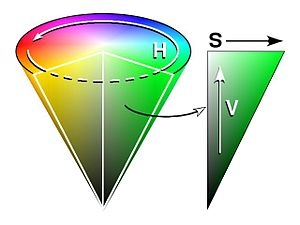
\includegraphics[width=6cm]{2_HSV.jpg}
	\caption{Stożkowa przestrzeń barw modelu HSV}
	\label{fig:HSV_cone}
\end{figure}

Poniższe wzory opisują sposób wyznaczenia poszczególnych składowych przestrzeni HSV w oparciu o RGB:

\begin{equation}
\label{HSV_first}
V=max(R,G,B)
\end{equation}

\begin{equation}
S=\begin{cases}
\frac{V-min(R,G,B)}{V}, & V\neq0 \\
0, & V=0
\end{cases}
\end{equation}

\begin{equation}
\label{HSV_last}
H=\begin{cases}
	0, & \text{jeśli } V-min(R,G,B)==0 \\
	\frac{60(G-B)}{V-min(R,G,B)}, & \text{jeśli } V==R \\
	\frac{60(B-R)}{V-min(R,G,B)}+120, & \text{jeśli } V==G \\
	\frac{60(R-G)}{V-min(R,G,B)}+240, & \text{jeśli } V==B 
\end{cases}
\end{equation}

\subsection{Wektor MeanShift}
\label{ssec:MS}
Istotą działania algorytmu MeanShift jest wyznaczanie maksimum funkcji gęstości w kolejnych iteracjach. Dla określanego obszaru obliczany jest środek masy punktów, do którego po zakończeniu algorytmu jest przesuwane aktualne położenie środka. To przesunięcie nosi nazwę \textit{wektora MeanShift}, który dla zbioru \textit{n} punktów $\{x_{i}\}_{i=1..n}$ oraz środka obszaru w punkcie $y_0$ może zostać zapisany jako:

\begin{equation}
\label{eq:ms1}
M(y)=\bigg[\frac{1}{n}\mathlarger{\sum\limits_{i=1}^{n}}x_i\bigg]-y_0
\end{equation}

Prostota wzoru \ref{eq:ms1} wynika z ujednolicenia wagi dla wszystkich punktów. Wprowadzając wagę punktu zależną od jego odległości od środka obszaru - takiej, która maleje wraz z oddalaniem się od centrum), wzór \ref{eq:ms1} można przepisać jako:

\begin{equation}
\label{eq:ms2}
M(y)=\frac{\sum_{i=1}^{n}w_i(y_0)x_i}{\sum_{i=1}^{n}w_i(y_0)}-y_0
\end{equation}
W równaniu \ref{eq:ms2}, $w_i(y_0)$ są wagami dla poszczególnych punktów.

Rysunek  \ref{fig:ms_vector} ilustruje przykładowe wygenerowanie wektora MeanShift, gdzie niebieskim okręgiem zaznaczono obszar podlegający działaniu algorytmu. Wszystkie punkty mają tu jednak identyczną wagę.
\begin{figure}[h]
	\centering
	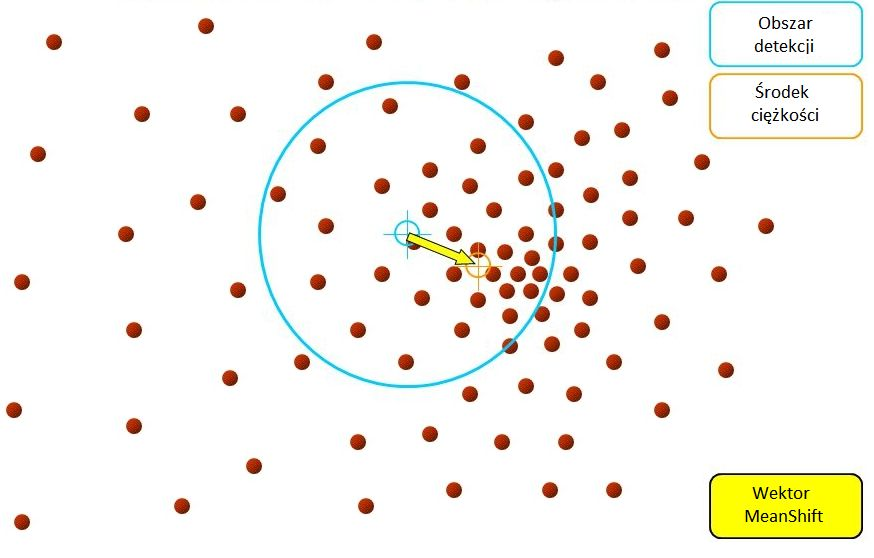
\includegraphics[width=10cm]{2_meanshift.jpg}
	\caption{Graficzna interpretacja wektora MeanShift \cite{Egorov}}
	\label{fig:ms_vector}
\end{figure}

\subsection{Jądro obszaru}
Celem wyznaczenia jądra (ang. \textit{kernel}) dla obszaru o stałej wielkości jest przypisanie najwyższej wagi punktom, które znajdują się najbliżej środka obszaru. Konsekwencją tego jest nadawanie znikomych wag punktom na jego rubieżach. Postać jądra zwykle przyjmuje klasyczne postacie gęstości rozkładów probabilistycznych: między innymi rozkładu jednorodnego (wagi jednakowe), prostokątnego, Gaussa, Cauchy'ego, Epanechnikova. W niniejszej pracy zdecydowano się wykorzystać jądro trójkątne ze względu na jego dobre wyniki i jednoczesną prostotę implementacji, nie bez znaczenia podczas późniejszej ealizacji sprzętowej w układzie FPGA. Jądro takie można opisać poniższym wzorem:

\begin{equation}
\label{eq:ms3}
K(u)=\begin{cases}
1-\frac{u}{b}, & \text{jeśli }\frac{u}{b}\leq 1 \\
0, & \text{jeśli }\frac{u}{b} > 1
\end{cases}
\end{equation}
gdzie $u$ jest odległością pomiędzy punktem a środkiem obszaru, a $b$ jest połową jego boku (zakładając, że obszarem jest kwadrat). Rysunek \ref{fig:kernel} przedstawia jądro o wymiarach 100x100 - w punkcie (50,50) osiąga maksymalną wartość 1 (natomiast $u=0$).
\begin{figure}[h]
	\centering
	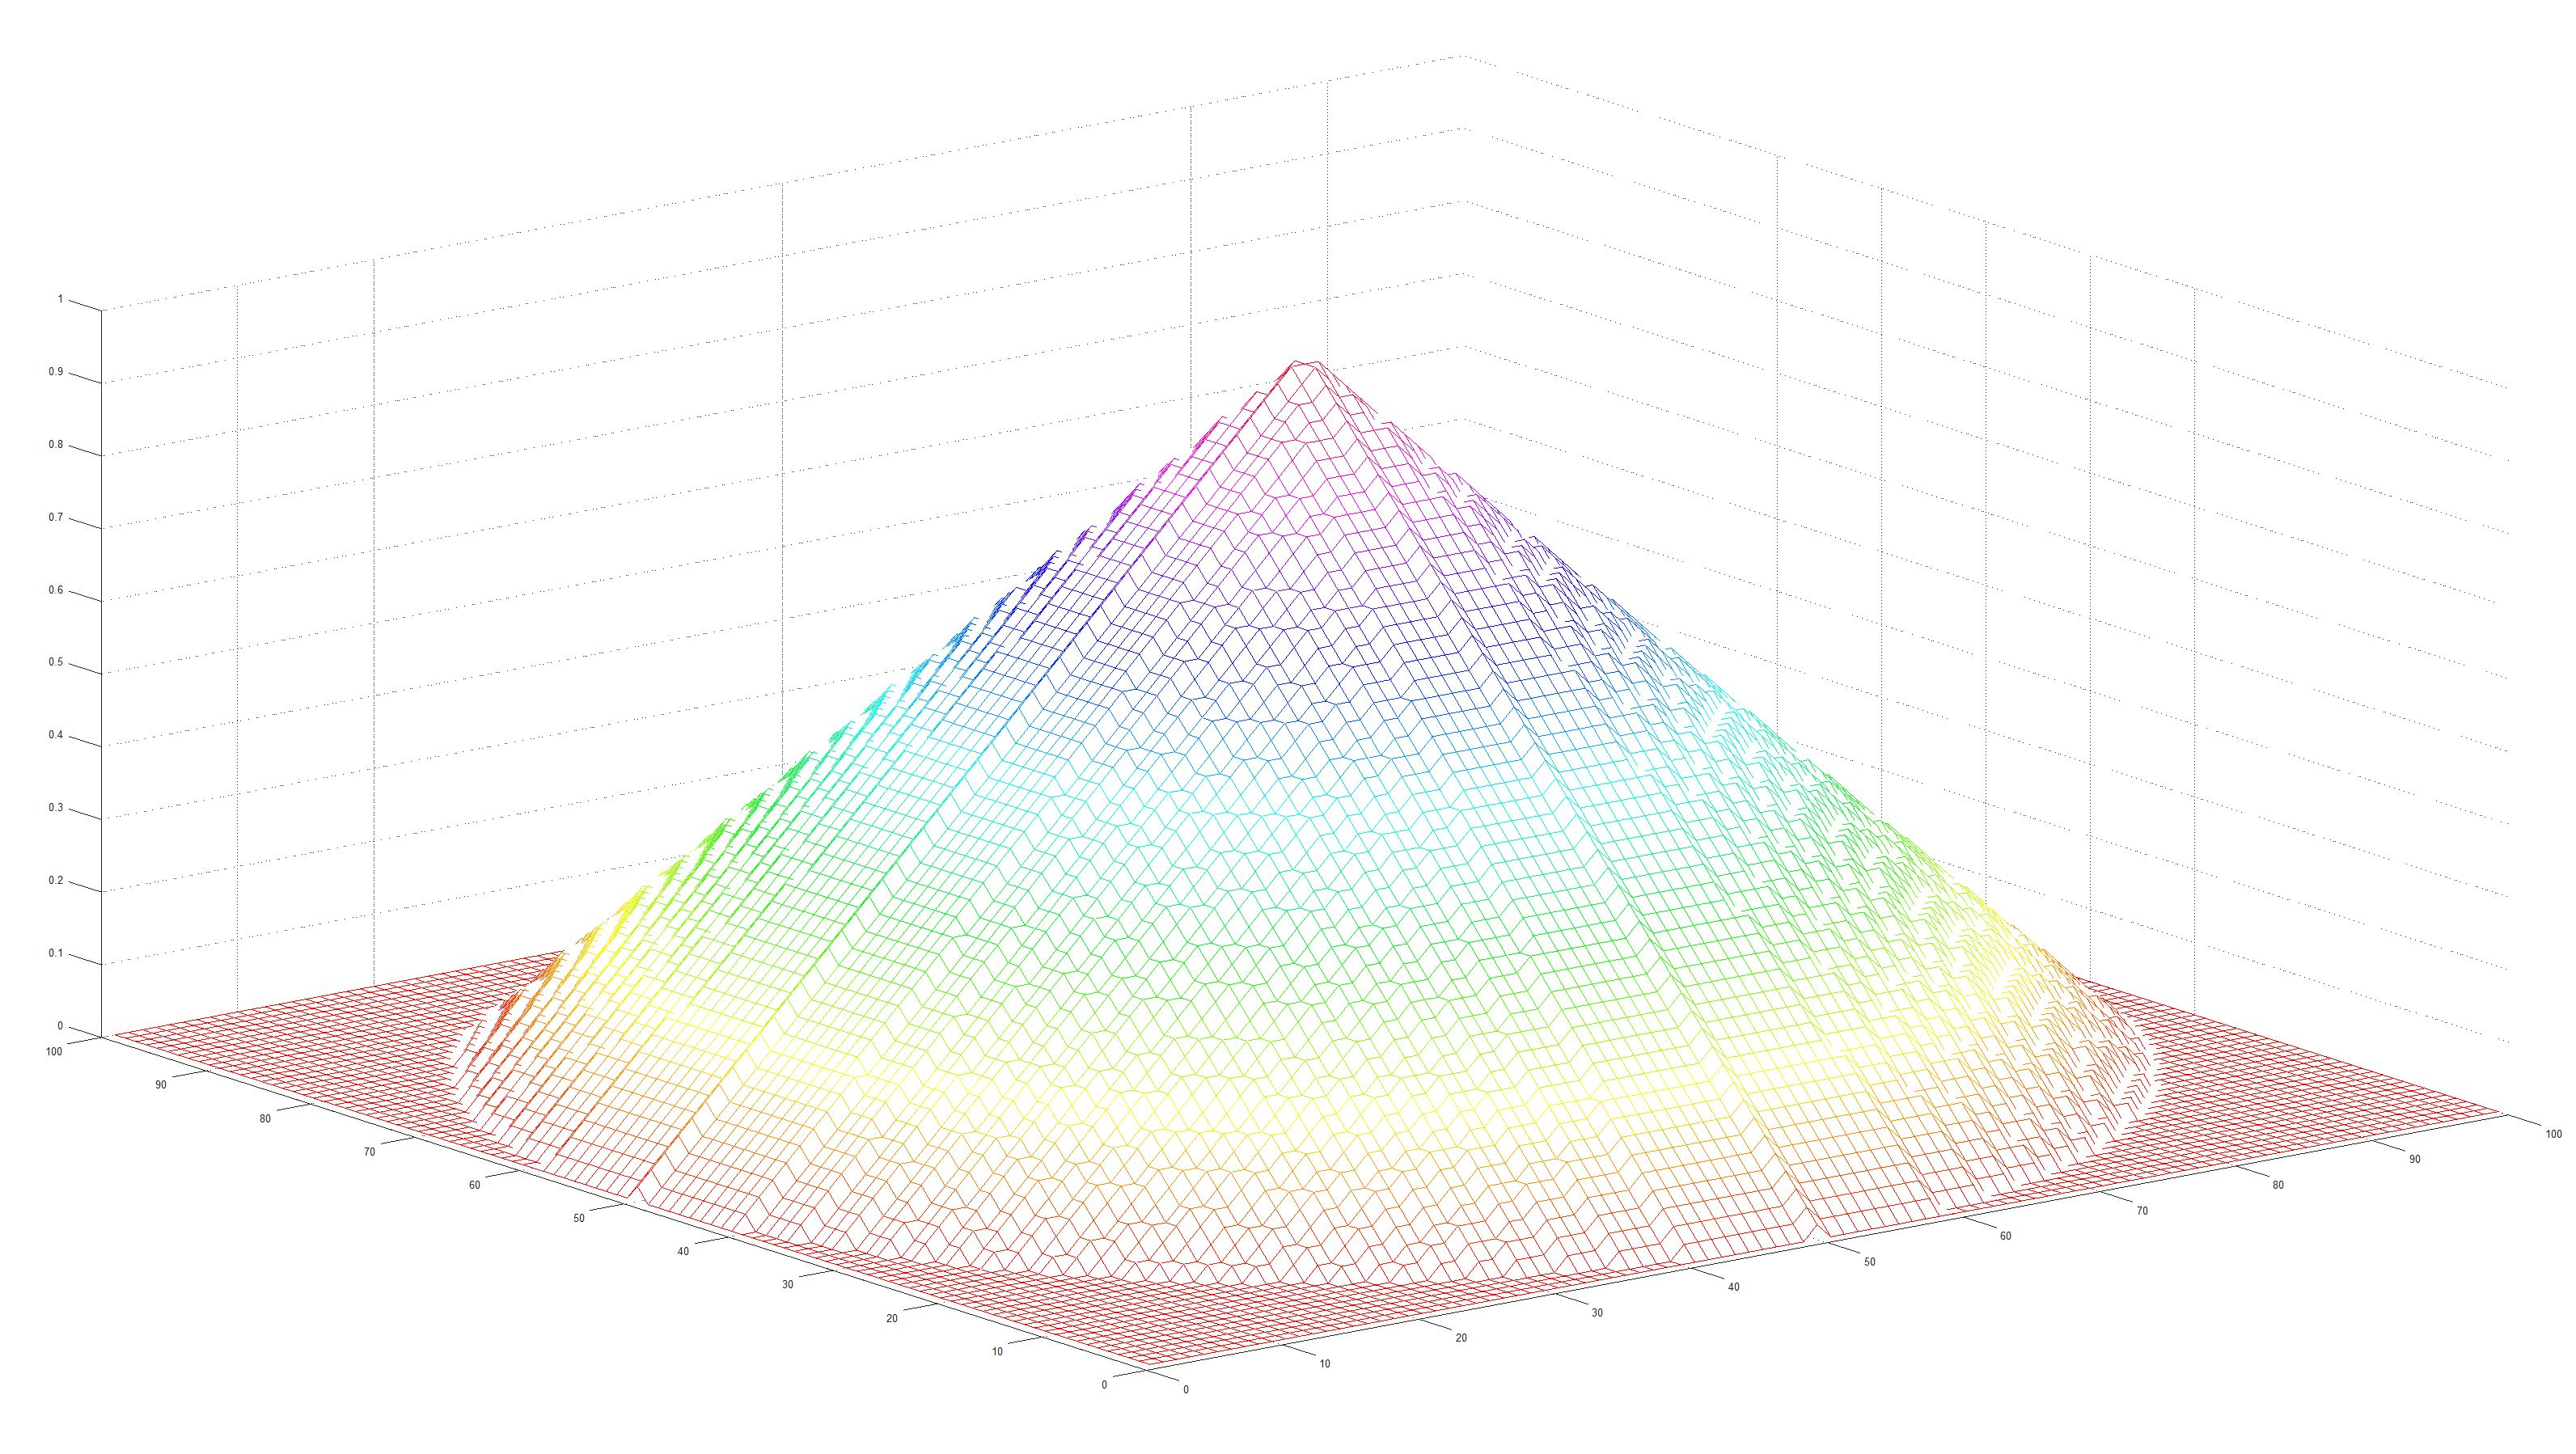
\includegraphics[width=16cm]{2_kernel.jpg}
	\caption{Jądro obszaru o wymiarach 100x100 (wygenerowane w programie MATLAB)}
	\label{fig:kernel}
\end{figure}

\subsection{Gęstość jądra}
Mając zbiór $n\times n$ punktów: $\{x_{i},y_{j}\}_{i=1..n,i=j..n}$ z przestrzeni $\mathbb{R}^2$ oraz jądro $K(u)$ dla punktu centralnego $P=(x,y)$ można przedstawić funkcję oszacowania gęstości:

\begin{equation}
\left.\begin{aligned}
f(P)&=\frac{1}{n^2}\sum_{i=1}^{n}\sum_{j=1}^{n}K(P-P'(i,j)) \\
f(P)&=\frac{1}{n^2}\sum_{i=1}^{n}\sum_{j=1}^{n}K(||P-P'(i,j)||).
\end{aligned}\right.
\end{equation}
Różniczkując powyższe otrzymuje się:
\begin{equation}
\label{eq:K}
\nabla f(P)=\frac{1}{n^2}\sum_{i=1}^{n}\sum_{j=1}^{n}(P-P'(i,j))K'(||P-P'(i,j)||),
\end{equation}
a po podstawieniu $g(x)$ za $-K'(x)$, wzór \ref{eq:K} może zostać zapisany jako:
\begin{equation}
\nabla f(x)=\frac{1}{n^2}\sum_{i=1}^{n}(P-P'(i,j))g(||P-P'(i,j)||),
\end{equation}
Po przekształceniu wzór może być przedstawiony jako:
\begin{equation}
\label{eq:kerms}
\begin{aligned}
\nabla f(x)= &\frac{1}{n^2}\bigg[\sum_{i=1}^{n}\sum_{j=1}^{n}g(||P-P'(i,j)||)\bigg] \cdot\\ \cdot&\bigg[\frac{\sum_{i=1}^{n}\sum_{j=1}^{n}P'(i,j)g(||P-P'(i,j)||)}{\sum_{i=1}^{n}\sum_{j=1}^{n}g(||P-P'(i,j)||)} -P\bigg],
\end{aligned}
\end{equation}
Ze wzoru \ref{eq:kerms} można wyodrębnić człon będący gradientem jądra: $g(P)=-K'(P)$. Drugą jego część stanowi wektor MeanShift z wagami odpowiadającymi wartościom gradientu jądra o środku w punkcie $x$. Zakładając niezerowość wyrażenia $\sum_{i=1}^{n}\sum_{j=1}^{n}g(||P-P'(i,j)||^2)$, wektor ten może przyjąć ostateczną formę:
\begin{equation}
M_s(P)=\frac{\sum_{i=1}^{n}\sum_{j=1}^{n}P'(i,j)g(||P-P'(i,j)||)}{\sum_{i=1}^{n}\sum_{j=1}^{n}g(||P-P'(i,j)||)} -P.
\end{equation}

\subsection{Współczynnik Bhattacharyya}
 \label{ssec:Bhat}
Zastosowanie algorytmu MeanShift do śledzenia obiektów na materiale
wideo wymaga znalezienia zależności pomiędzy funkcjami gęstości wzorca oraz kandydata. W tym celu należy zestawić ze sobą oba rozkłady na przykład za pomocą współczynnika Bhattacharyya, który dla $m$-wymiarowych funkcji gęstości wzorca $q_h$ oraz obszaru-kandydata $p_h$ ze środkiem w punkcie $P$ wyraża się wzorem:
\begin{equation}
\label{eq:Bhat}
\rho(P)=\sum_{h=1}^{m}\sqrt{p_h(P)q_h}
\end{equation}
Wyznaczenie przesunięcia obiektu na obrazie dla kolejnych klatek obrazu wymaga znalezienia maksymalnego współczynnika Bhattacharyya, co jest tożsame (według algorytmu) ze zidentyfikowaniem najbardziej podobnego fragmentu do oryginalnego obszaru śledzonego.

\subsection{Śledzenie}
Opisane wyżej jądro i jego gradient stanowią inicjalizację całego algorytmu i są obliczane jeszcze przed zdefiniowaniem wzorca. Cechą obrazu, dla której będzie liczona funkcja prawdopodobieństwa, jest kolor (H z przestrzeni barw HSV, jest to liczba z zakresu 0-359). 
Jeśli położenie piksela na obrazie wzorca oznaczone jest jako $\{x_{i},y_{j}\}_{i=1..n,i=j..n}$, niech zdefiniowana będzie funkcja $b:\mathbb{R}^2\rightarrow\{1..m\}$, która odwoływać się będzie do składowej \textit{H} danego piksela.

Barwa piksela jest przede wszystkim argumentem funkcji prawdopodobieństwa utworzonego dla \textit{H} na danym obszarze detekcji. Współczynnik Bhattacharyya jest \textit{de facto} porównaniem dwóch funkcji prawdopodobieństwa (wzorca i kandydata) o wymiarze cech równym 360.   
Podczas obliczania prawdopodobieństwa wystąpienia określonego koloru, istotną rolę odgrywać musi wartość jądra, które zwiększa wagę pikseli znajdujących się w centrum obszaru, marginalizując znaczenie tych brzegowych - które mogłyby być częścią zmiennego w czasie tła. O ile w tradycyjnym histogramie wartości przedziałów zwiększa się poprzez inkrementację, to w tym przypadku zdecydowano się na powiększenie o wartość jądra odpowiadającego położeniu piksela na obszarze 100x100.
 Dla przykładowej barwy $h$, funkcja gęstości prawdopodobieństwa może być zdefiniowana jako:
\begin{equation}
q_h=C\sum_{i=1}^{n}\sum_{j=1}^{n}K(||P-P'(i,j)||)\delta[b(P'(i,j))-h],
\end{equation}
gdzie $P$ to nadal środek obszaru detekcji a symbol $\delta$ jest deltą Kroneckera. Współczynnik $C$ odpowiada za normalizację $q_h$: $\sum_{h=1}^{m}q_h=1$.
Po przekształceniu okazuje się, że:

\begin{equation}
C=\frac{1}{\sum_{i=1}^{n}\sum_{j=1}^{n}K(||P-P'(i,j)||)} 
\end{equation}

W każdej iteracji dla kandydata wyznacza się funkcję gęstości prawdopodobieństwa. Uwzględniając obszar ze środkiem w punkcie $P$, wzór prezentuje się następująco:
\begin{equation}
\label{eq:density}
p_h(P)=C_k\sum_{i=1}^{n}\sum_{j=1}^{n}K(||P-P'(i,j)||)\delta[b(P'(i,j))-h] 
\end{equation}

Współczynnik $C_h$ wyznacza się podobnie, jak dla wzorca, jednak z uwgzlędnieniem położenia środka obszaru kandydata, $P$:
\begin{equation}
C_k=\frac{1}{\sum_{i=1}^{n}\sum_{j=1}^{n}K(||P-P'(i,j)||)} 
\end{equation}
Następnie należy zbadać podobieństwo obu rozkładów gęstości - wykorzystywany jest w tym celu współczynnik Bhattacharyya, opisany w rozdziale \ref{ssec:Bhat}. Rozwijając wzór \ref{eq:Bhat} w szereg Taylora ze środkiem obszaru wzorca równym $P_0$ można otrzymać:
\begin{equation}
\label{eq:approx}
\rho(p(P),q)\approx\frac{1}{2}\sum_{u=1}^{m}\sqrt{p_u(P_0)q_u} + \frac{1}{2}\sum_{u=1}^{m}p_u(P)\sqrt{\frac{q_u}{p_u(P_0)}}
\end{equation}
Podstawienie równania \ref{eq:density} do powyższego wyrażenia daje:
\begin{equation}
\label{similarity_est}
\begin{aligned}
\rho(p(P),q)\approx & \frac{1}{2}\sum_{u=1}^{m}\sqrt{p_u(P_0)q_u} + \\ & \frac{C_k}{2}\sum_{i=1}^{n}\sum_{j=1}^{n}\sum_{u=1}^{m}\sqrt{\frac{q_u}{p_u(P_0)}}\delta[b(P'(i,j))-h] k(||P-P'(i,j)||)
\end{aligned}
\end{equation}
Stąd można wyodrębnić:
\begin{equation}
\label{eq:wi}
w_{i,j}=\sum_{u=1}^{m}\sqrt{\frac{q_u}{p_u(P_0)}}\delta[b(P'(i,j))-h]
\end{equation}


We wzorze \ref{similarity_est} pierwsza składowa jest niezależna od położenia środka obszaru kandydata $P$. Maksymalizując funkcję podobieństwa, należy skupić się na poszukiwaniu największej wartości drugiego członu. 
Wykorzystując wektor MeanShift z rozdziału \ref{ssec:MS} z wagami równymi wartościom funkcji podobieństwa wzorca i kandydata oraz wzór \ref{eq:wi}, dla każdej klatki obrazu i w każdej iteracji należy wyliczyć aktualne położenie obszaru w oparciu o względne przesunięcie dane poniższym wzorem.

\begin{equation}
\label{eq:position}
\Delta P=\frac{\sum_{i=1}^{n}\sum_{j=1}^{n}P(i,j)\cdot w_{i,j}\cdot g(P-P'(i,j))}{\sum_{i=1}^{n}\sum_{j=1}^{n}w_{i,j}\cdot g(||P-P'(i,j)||)}
\end{equation}

\subsection{Warunki zakończenia algorytmu}
W przypadku algorytmu iteracyjnego konieczne jest zdefiniowanie celów, które należy osiągnąć. Uzyskanie całkowitego podobieństwa pomiędzy wzorcem i kandydatem w zmiennej sekwencji obrazów raczej nie jest do osiągnięcia. Chcąc przetwarzać obraz w czasie rzeczywistym, należy zakończyć przetwarzanie klatki przed momentem, w którym dane z następnej będą gotowe. Stąd dwa podstawowe warunki zakończenia algorytmu to:
\begin{enumerate}
	\item numer iteracji == maksymalna liczba iteracji
	\item $||y_{n_m}-y_{n_{m-1}}||==0$,
\end{enumerate} 
gdzie $n$ jest liczbą porządkową klatki, a $m$ jest numerem iteracji algorytmu MeanShift dla konkretnej klatki.
W momencie spełnienia jednego z powyższych warunków, akceptuje się dotychczasowo uzyskaną zmianę położenia obszaru detekcji i rozpoczyna obliczenia następnej klatki. \newline Rysunek \ref{fig:MS_diagram} przedstawia diagram algorytmu MeanShift dla sygnału wideo.
\begin{figure}
	\centering
	\hspace*{-3cm}
	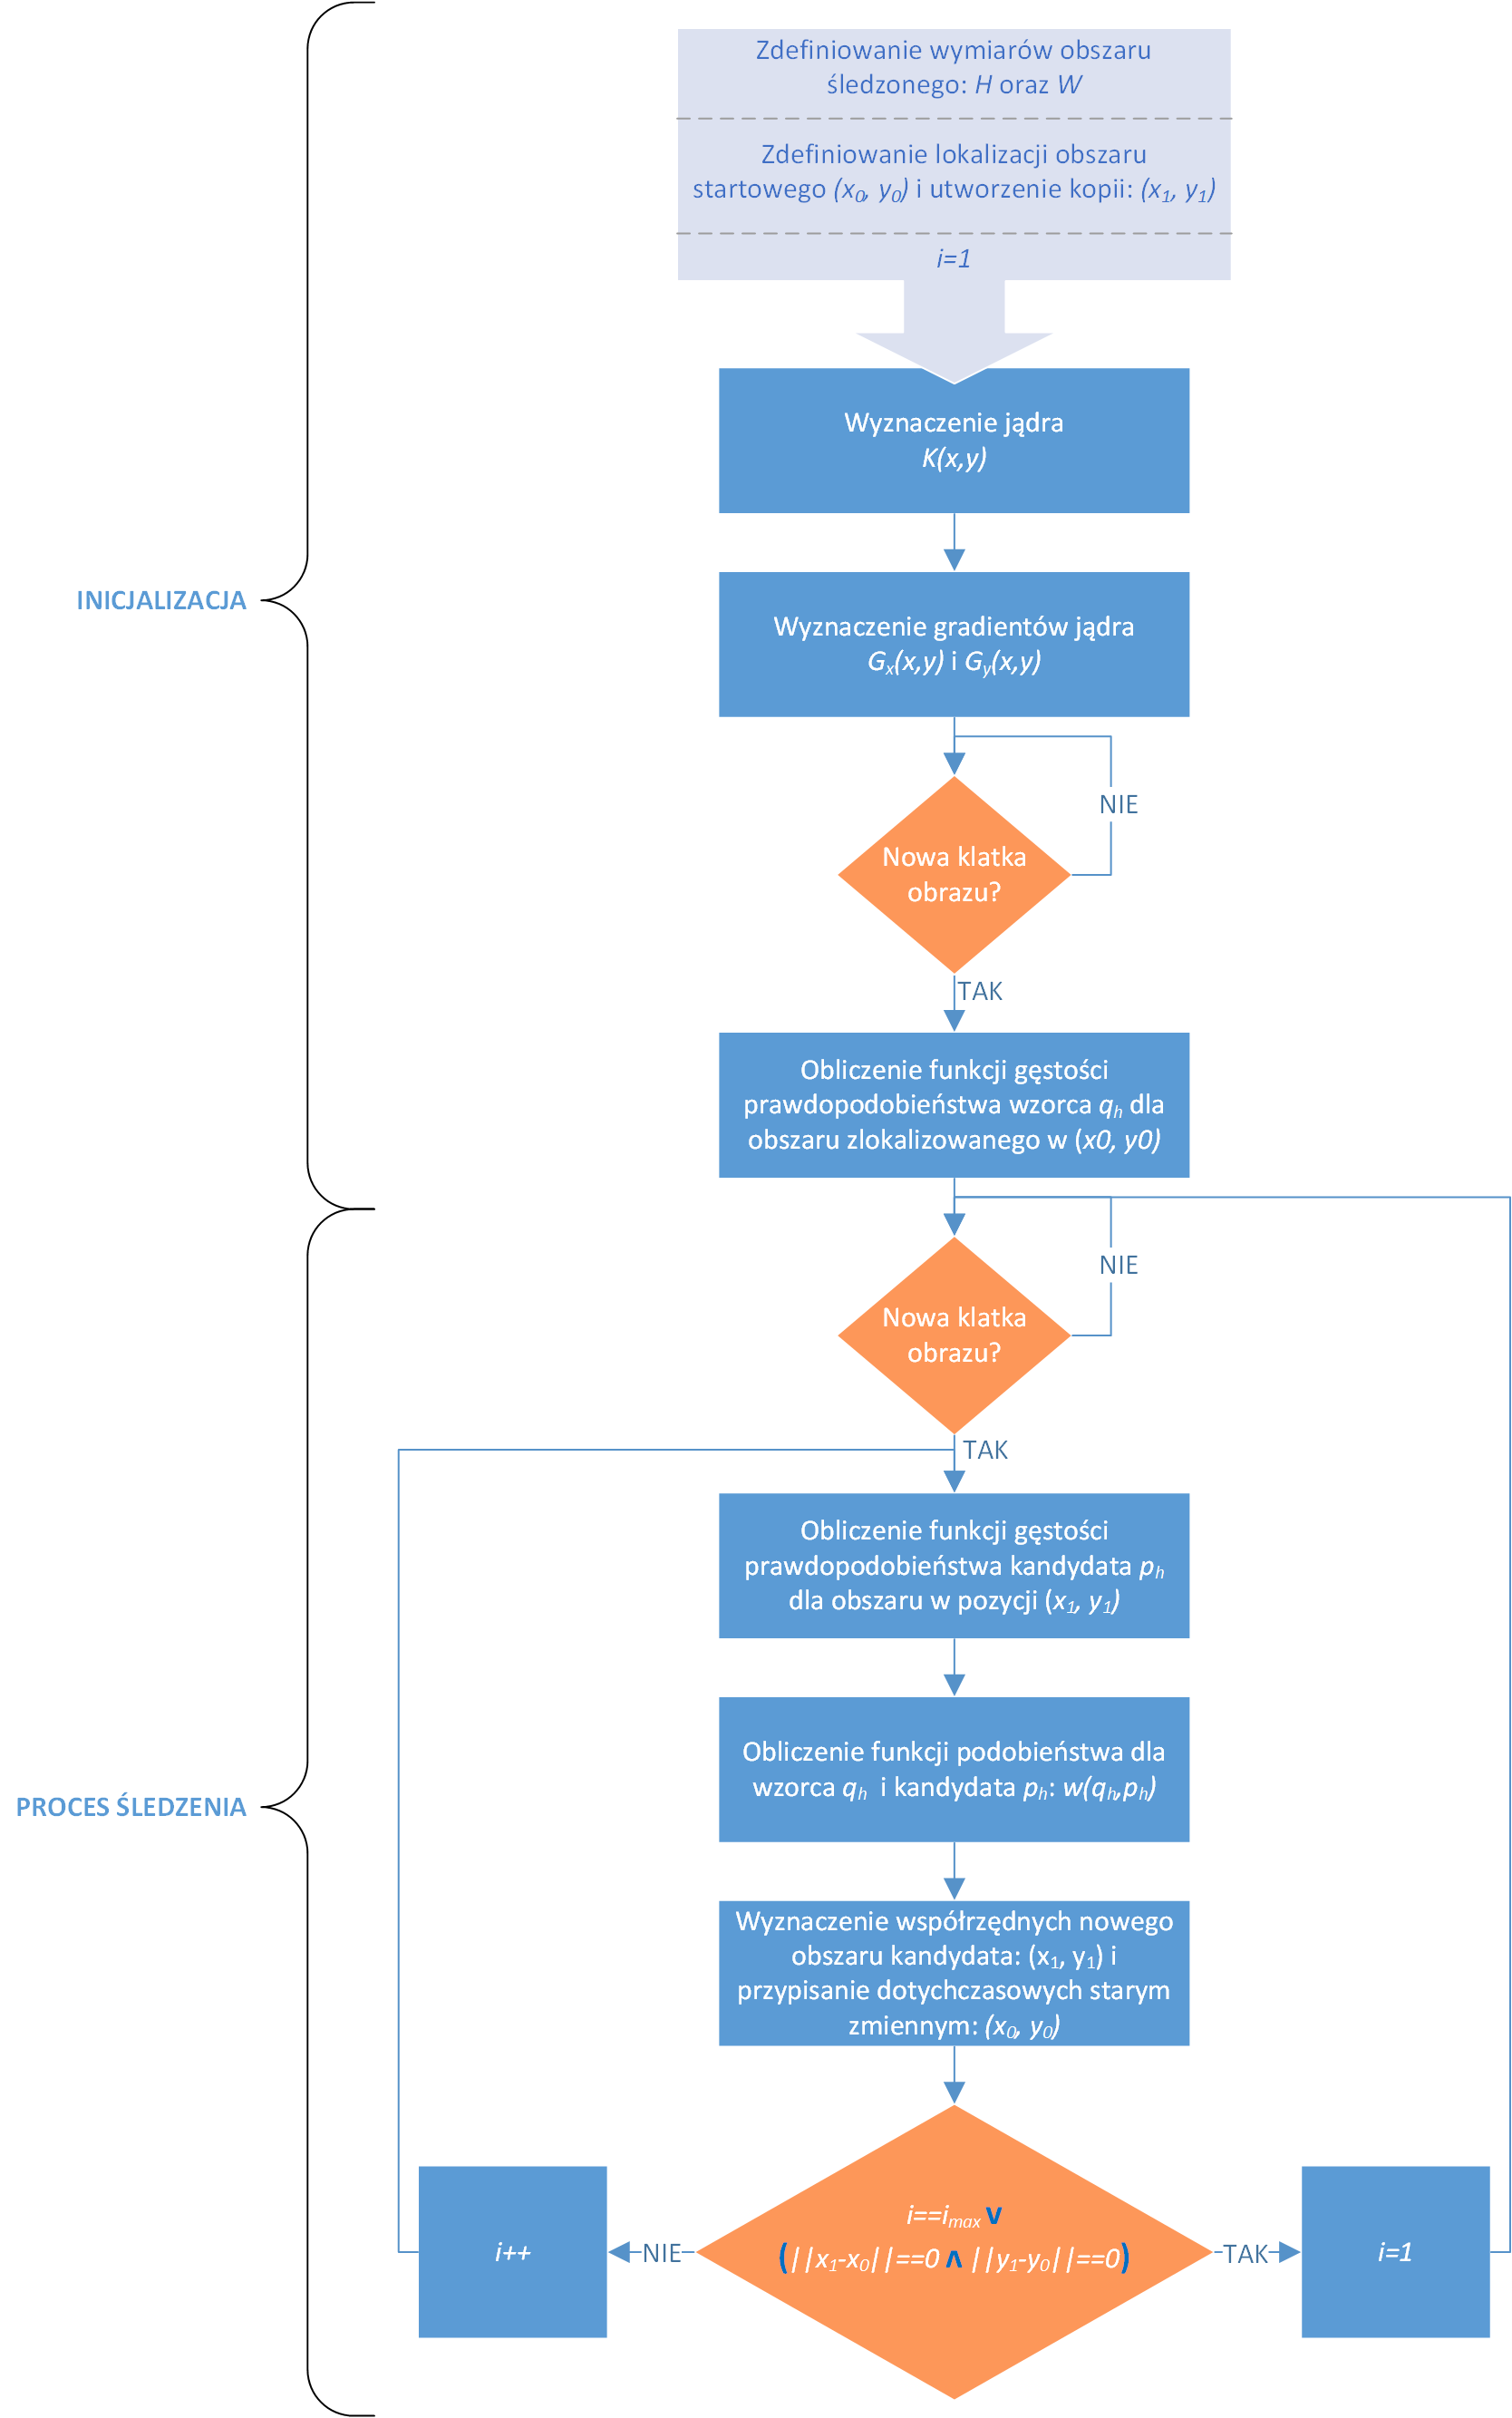
\includegraphics[width=14.5cm]{2_MS_visio.png}
	\caption{Schemat blokowy algorytmu MeanShift}
	\label{fig:MS_diagram}
\end{figure}

\section{Algorytm HOG+SVM}
\label{sec:HOG&SVM}
Inną gradientową metodą detekcji (oraz śledzenia) jest algorytm wykorzystujący zestaw cech obrazu - konkretnie histogram ukierunkowanych gradientów (ang. \textit{Histogram of Oriented Gradients - HOG}); rolę decyzyjną pełni klasyfikator nazywany maszyną wektorów nośnych (ang. \textit{Support Vector Machine - SVM}). Pierwotnie, ten rodzaj hybrydy został przedstawiony w pracy [Dalal and Triggs, 2005], z zastosowaniem w detekcji pieszych, co może czynić go wystarczająco dopasowanym do potrzeb niniejszego projektu. Oczywiście należy dodać, że dysponując odpowiednim zestawem informacji, odpowiednio trenowany mechanizm SVM byłby w stanie działać z innymi obiektami.

\subsection{Konwersja RGB->GRAY i kąty gradientów}
\label{sec:HOGgrad}
Pierwszym etapem jest dostosowanie pierwotnej palety barw RGB do 8-bitowej skali szarości. Dokonuje się tego, przekształcając każdy piksel według wzoru:
\begin{equation}
\label{eq:rgb2gray}
P_{GRAY}=0.299P_R + 0.587P_G + 0.114P_B 
\end{equation}
Sumowanie się współczynników do jedności ma w zamierzeniu ograniczyć wynik tego przekształcenia do zakresu 0-255.

Następnie przeprowadzana jest operacja kontekstowa w celu obliczenia gradientów kierunkowych $g_x$ oraz $g_y$; używane maski to odpowiednio: $[-1,0,1]$ oraz $[-1,0,1]^T$. 
Mając gradienty, dla każdego piksela (o koordynatach [$i,j$]) obliczany jest także moduł i kąt ze wzorów:

\begin{equation}
\label{eq:HOGangles}
\left.\begin{aligned}
m(i,j)=\sqrt{g_x(i,j)^2+g_y(i,j)^2} \\
\theta(i,j)=arctg\bigg(\frac{g_y(i,j)}{g_x(i,j)}\bigg)
\end{aligned}\right.
\end{equation}

\subsection{Histogram gradientów}
W kolejnym etapie poddawany przetwarzaniu obraz będzie dzielony na kwadratowe obszary (dla jasności nazywane od teraz \textit{komórkami}) o wymiarach 4x4, 8x8 czy 16x16 pikseli. W każdej z komórek zostanie wyliczony niezależny histogram na podstawie kątów gradientu. Oprócz rozmiaru komórki, kluczowym okazuje się również drugi parametr, czyli ilość przedziałów klasowych pojedynczego histogramu - w tym wypadku zdecydowano, by rozpatrywany kąt przyporządkowywać jednemu z 9 przedziałów równo dzielących zakres $[0^{\circ},180^{\circ})$ - i komplementarnie $[-180,0)$. Wynika z tego, że każdy kolejny zakres $a=180/9=20^{\circ}$ będzie stanowić osobny przedział klasowy histogramu.

O ile typowy histogram tworzony jest poprzez inkrementację odpowiedniego przedziału o 1, to tworzona struktura będzie wykorzystywać obliczony wcześniej moduł z gradientu. Dodatkowo, autorzy publikacji wspominają o możliwości interpolacji pomiędzy dwoma sąsiednimi przedziałami i inkrementacji poszczególnych wartości o proporcjonalne części modułu - takie działanie ma pozytywnie wpływać na wyniki detekcji. Jeśli zatem przyjąć, że $\theta_h$ i $\theta_l$ to wartości kątów będących środkami dwóch sąsiadujących ze sobą przedziałów, którym jednocześnie najbliżej do badanego kąta $\theta$, wówczas będzie można zdefiniować inkrementy $M_h$ i $M_l$ jako:

\begin{equation}
\label{eq:HOG_linear}
\left.\begin{aligned}
M_h(i,j)&=m(i,j)\bigg(\frac{\theta-\theta_l}{a}\bigg)\\
M_l(i,j)&=m(i,j)\bigg(\frac{\theta_h-\theta}{a}\bigg)
\end{aligned}\right.
\end{equation}
Ostatecznie, następuje powiększenie wartości dwóch odpowiednich przedziałów histogramu $H$ tworzonego w obrębie komórki zawierającej piksel o współrzędnych (i,j):

\begin{equation}
\label{eq:HOG_increment}
\left.\begin{aligned} 
H(\theta_h,i,j)&=H(\theta_h)+M_h(i,j) \\ 
H(\theta_l,i,j)&=H(\theta_l)+M_l(i,j)
\end{aligned}\right.
\end{equation}

Przykładem może być sytuacja przedstawiona na rysunku \ref{fig:HOG_interpolation}. Wyjątkowym zdarzeniem jest takie, w którym kąt $\theta$ będzie znajdował w okolicy kąta $0^{\circ}=360^{\circ}$ (z przedziałami 1 oraz 9). Wówczas, dla wygody, w równaniach \ref{eq:HOG_linear} należy użyć kątów $\theta_l=350^{\circ}$ oraz $\theta_h=370^{\circ}$.

\begin{figure}[h]
	\centering
	\hspace*{1cm}
	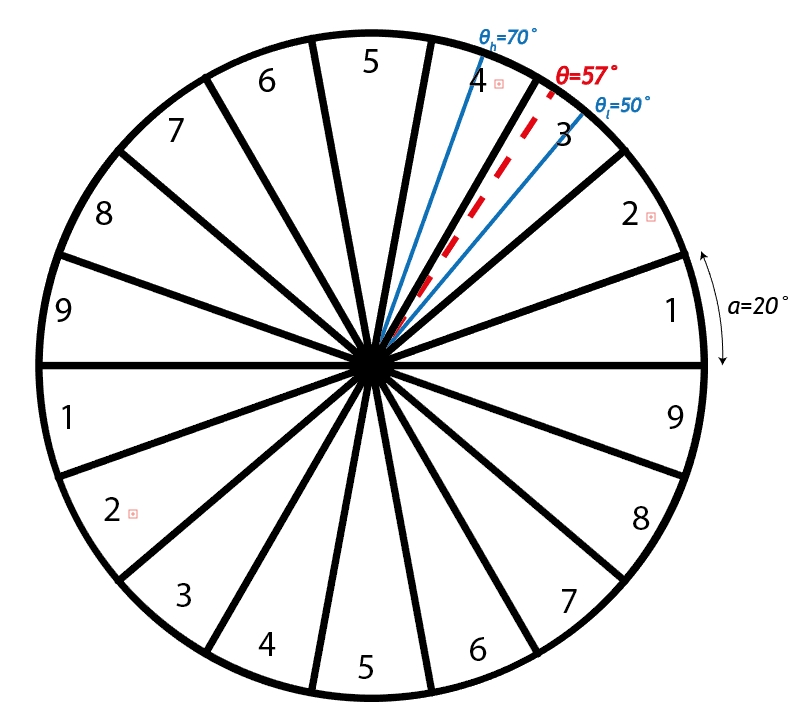
\includegraphics[width=12cm]{2_HOG_interpolation.jpg}
	\caption{Przykładowy problem liniowej interpolacji}
	\label{fig:HOG_interpolation}
\end{figure}

\subsection{Normalizacja}
Zazwyczaj, analizowany materiał wideo będzie nagrywany w amatorskich warunkach, co może w efekcie oznaczać nierówny poziom oświetlenia poszczególnych fragmentów obrazu. Zdegenerowany w ten sposób obraz nie dawałby dobrych wyników działania algorytmu. Z tego powodu proponuje się stosowanie blokowej normalizacji. 

Proponowane podejście zakłada utworzenie struktur nazywanych \textit{blokami}, gdzie każdy z nich obejmować ma $2\times 2$ sąsiednie komórki. Dla obrazu, na bazie którego utworzono $N \times M$ komórek, powinno powstać $N-1 \times M-1$ bloków - przy ich generowaniu wykonuje się krok o jedną komórkę w poziomie i/lub w pionie względem poprzedniego obszaru. Rozmiar pojedynczego bloku sugeruje, że będzie się on składał z 4 histogramów, w formie wektora: 
\begin{equation}
v=[H_{i,j}, H_{i,j+1}, H_{i+1,j}, H_{i+1,j+1}],
\end{equation} 
gdzie $i$  wiersz, $j$ - kolumna. Następnie należy obliczyć wektor cech $L$, wykorzystując jedną z sugerowanych zależności:

\begin{equation}
\label{eq:HOG_norm1}
\left.\begin{aligned} 
L1&=\frac{v}{\sum_{i}^{n}v_i+\epsilon}
\end{aligned}\right.
\end{equation}

\begin{equation}
\label{eq:HOG_norm2}
\left.\begin{aligned} 
L1_{sqrt}&=\frac{v}{\sqrt{\sum_{i}^{n}v_i+\epsilon}}
\end{aligned}\right.
\end{equation}

\begin{equation}
\label{eq:HOG_norm3}
\left.\begin{aligned} 
L2&=\frac{v}{\sqrt{\sum_{i}^{n}v_i^2+\epsilon^2}}
\end{aligned}\right.
\end{equation}

\begin{equation}
\label{eq:HOG_norm4}
\left.\begin{aligned} 
L2_{hys}&=\frac{v}{\sqrt{\sum_{i}^{n}v_i^2+\epsilon^2}}, v\leq 0.2
\end{aligned}\right.
\end{equation}
W powyższych równaniach $\epsilon$ to stała o małej wartości, a $n$ to liczba elementów w bloku (4 histogramy po 9 przedziałów $\rightarrow$ 36). Wektory $L$ zebrane z całego okna detekcji budują ostateczny wektor cech, na którym pracować będzie klasyfikator.

Niech podsumowaniem rozważania będzie przykład - obraz o rozmiarze $720\times 1280$ i komórka o wielkości $8 \times 8$. Wynikiem opisywanej procedury będzie utworzenie aż $90\cdot160=14400$ komórek i $89\cdot 159=14151$ bloków. Po normalizacji, klasyfikator otrzymałby aż $14151\cdot36=509436$ wartości do przetworzenia. Tak duża wartość niosłaby jednak za sobą konieczność optymalizacji, co będzie rozważone w rozdziale poświęconym implementacji algorytmu.

\subsection{Klasyfikator SVM}
Maszyna wektorów nośnych to klasyfikator binarny, który dzięki swej prostocie i skuteczności jest powszechnie wykorzystywany w procesie odróżniania klas. Jego działanie tradycyjnie można podzielić na dwie fazy: uczenie i klasyfikację. \newline Etap uczenia to relatywnie dłuższy czasowo proces wyznaczenia hiperpłaszczyzny, która z jak najlepszym marginesem rozdzieli wejściowe wektory cech obiektów klasyfikowanych jako \textit{1} od tych określonych jako \textit{0} (umownie). Stosowane podeście nie powinno odbiegać od klasycznej metodologii uczenia maszynowego - dysponując zbiorem danych wejściowych, należy dokonać podziału na próbki trenujące oraz testowe (w stosunku około 70:30). Każdy z z tych podzbiorów (a przede wszystkim trenujący) powinien posiadać zarówno obiekty zdefiniowane jako pozytywne, jak i negatywne. W niniejszej pracy, która ma na celu rozpoznanie osoby w postawie stojącej, wymagane będą obrazy przedstawiające taką postać w jak największej liczbie kombinacji (ale w podobnej skali), lecz także obrazy będące czymkolwiek innym, wyraźnie odmiennym od ludzkiej postaci. Dla poprawienia ostatecznych wyników należy zadbać również o zróżnicowanie obrazów pod kątem poziomu oświetlenia, a nawet tła otaczającego postać.\newline Etapem klasyfikacji nazwać można wykorzystanie otrzymanych w procesie uczenia parametrów do wyznaczenia położenia badanego wektora cech względem hiperpłaszczyzny. Na tej podstawie do obiektu zostanie przydzielona odpowiednia klasa.

\subsection{Idea skalowania obrazu}
Klasyfikator jest w stanie rozpoznać postać na obrazie $128\times 64$, jeśli jest tam obecna dość ogólnie nakreślonych proporcjach. Jednym z założeń systemu jest możliwość określenia odległości kamery od rozpoznanej osoby, by odpowiednio wpłynąć na sterowanie związane z tym kierunkiem. Skutecznym rozwiązaniem okazuje się być zastosowanie algorytmu HOG+SVM na kilku przeskalowanych w różny sposób kopiach obrazu. Z każdej skali należy wydobyć próbki obrazów o wymiarach $128\times 64$ i spróbować znaleźć najlepszą pozytywną detekcję. Odpowiadająca wybranemu wynikowi skala da pośrednią informację o odległości. Opisują to rysunki poniżej.
\begin{figure}[h]
	\centering
	\captionsetup{justification=centering,margin=1cm}
	\hspace*{0cm}
	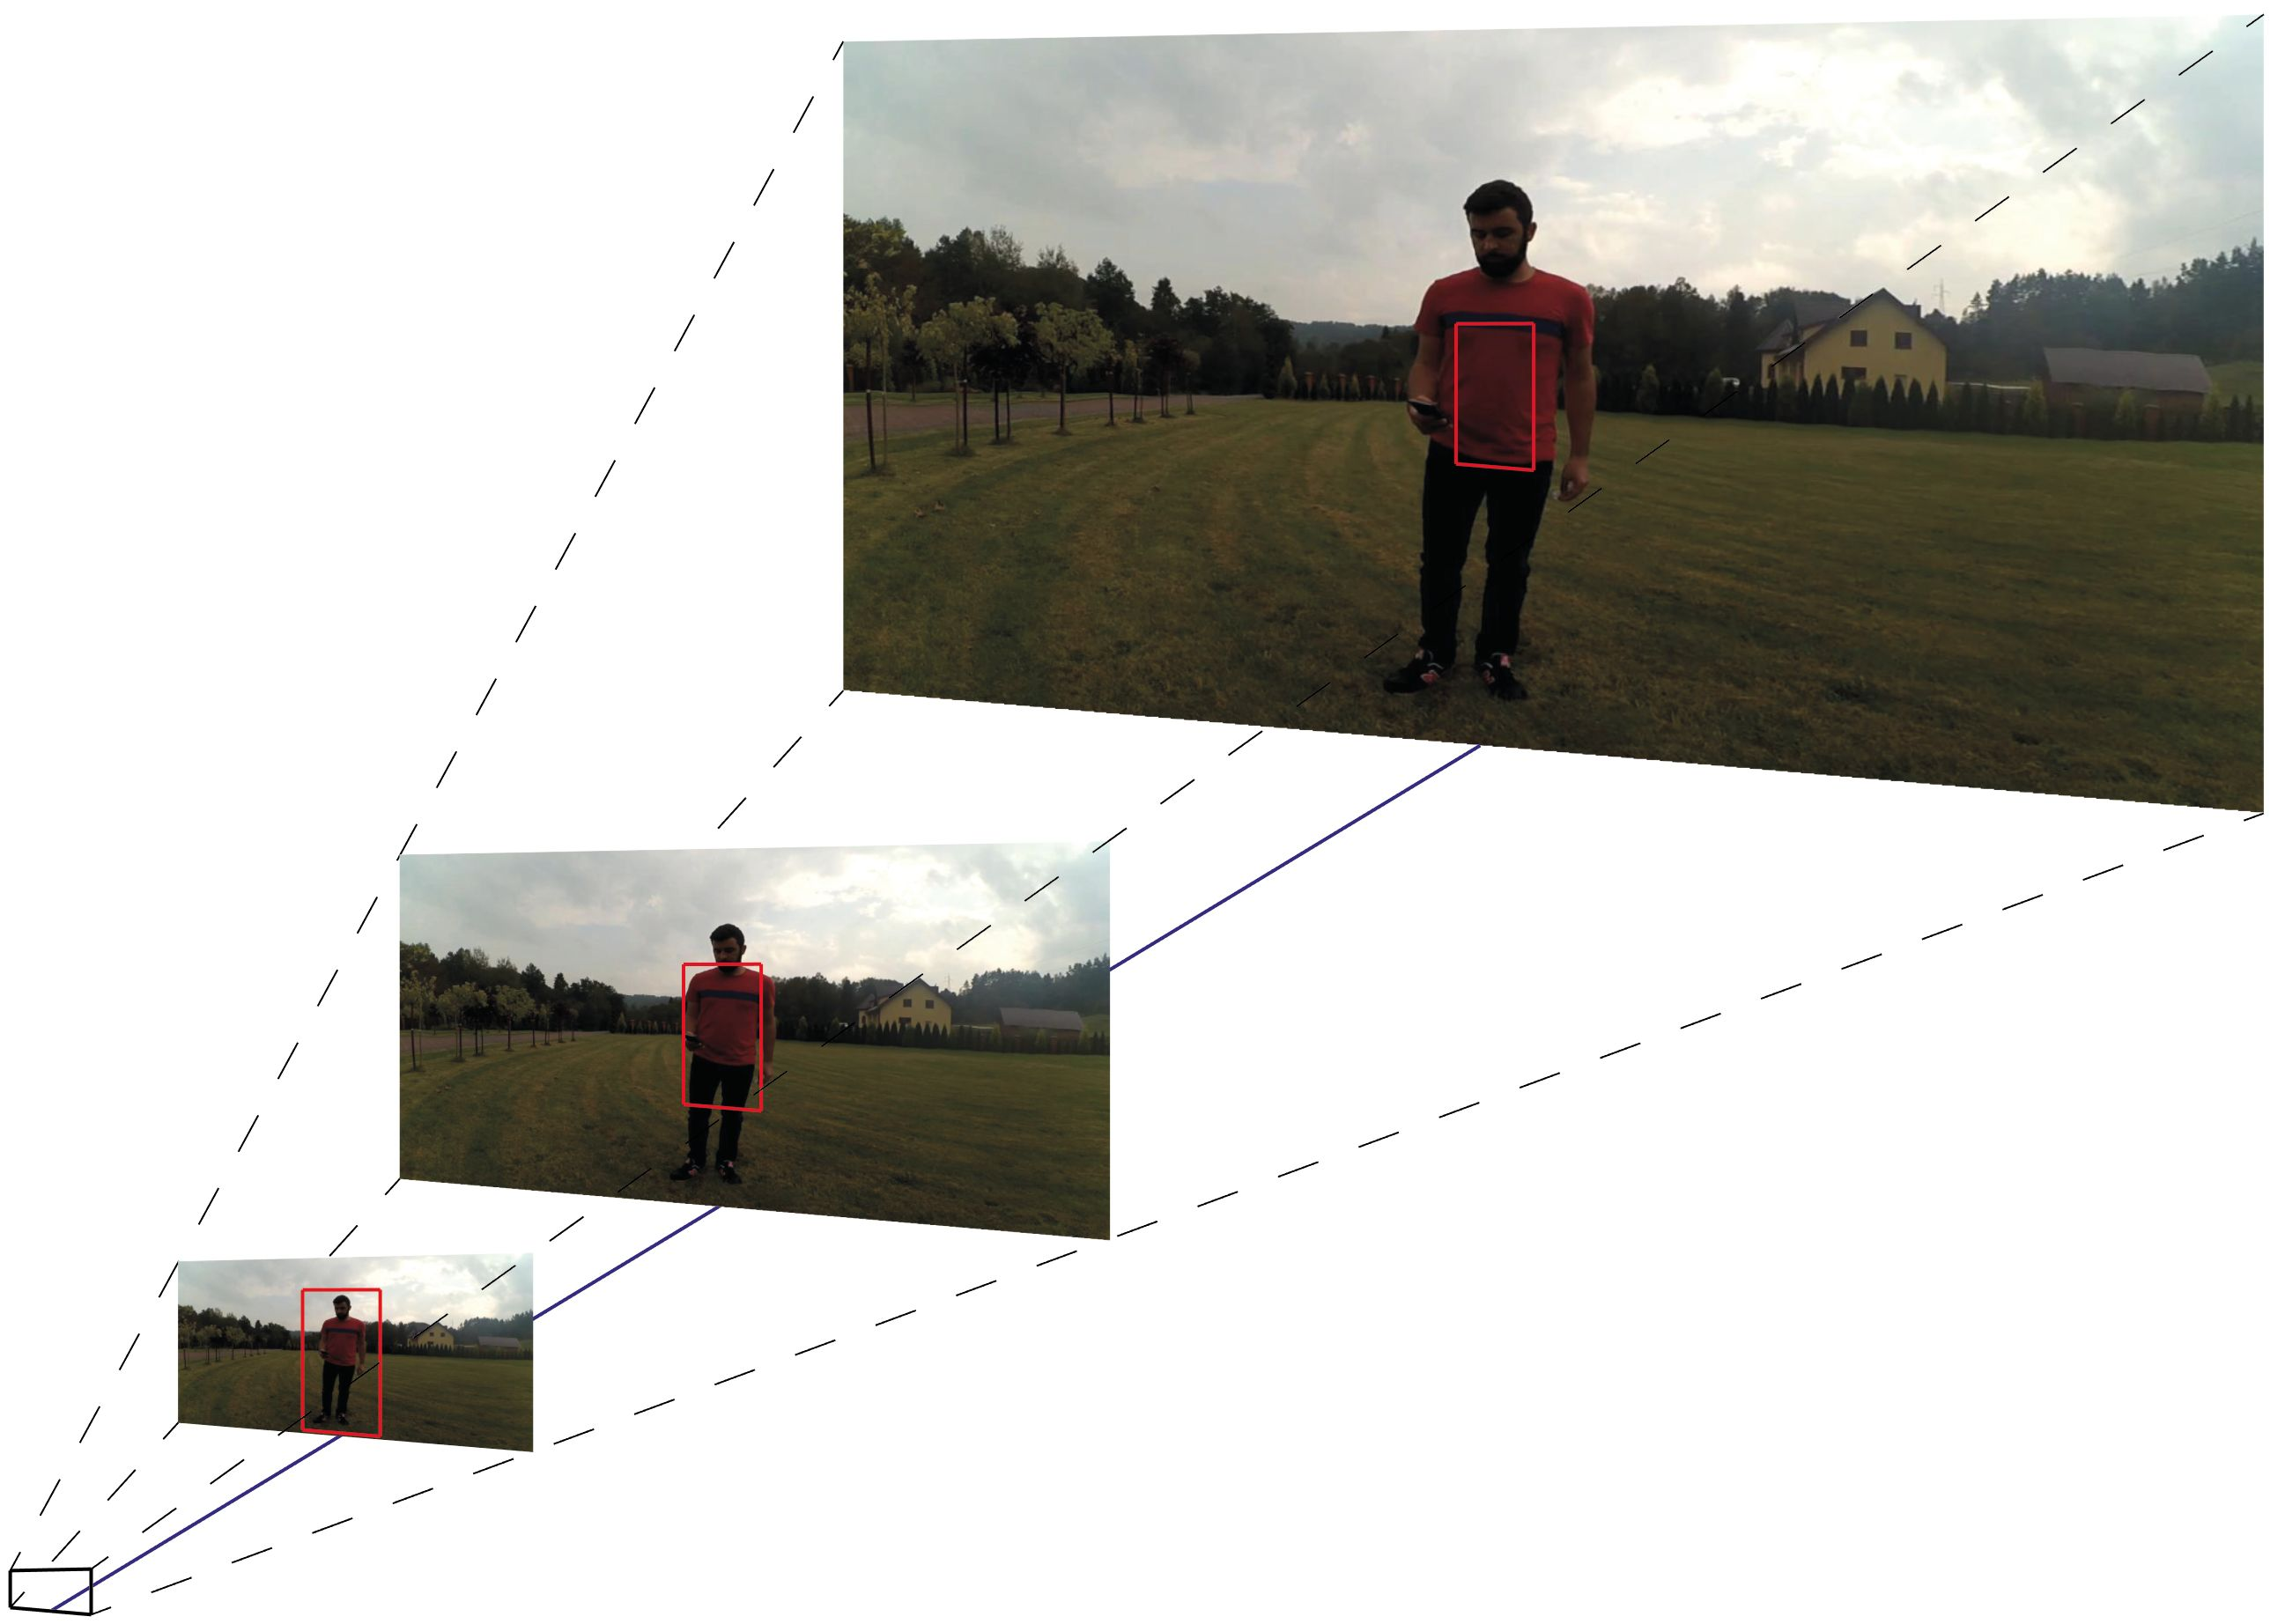
\includegraphics[width=15.5cm]{2_scaling.jpg}
	\caption{Skalowanie 1:1, 1:2 oraz 1:4 z naniesionym przykładowym oknem detekcji $128 \times 64$}
	\label{fig:HOG_image_examples}
\end{figure}
\newline
Widoczne na rysunku okno detekcji nasuwa wniosek, że osoba wykryta na oryginalnym obrazie będzie znacząco oddalona od kamery. Najbliżej rozpoznania postaci jest okno detekcji na obrazie przeskalowanym w stosunku 1:4.
Znając przybliżoną pozycję osoby wykrywanej przez takie okno na oryginale i stosując proste twierdzenie Talesa, można oszacować odległość. Opisuje to poniższy wzór:
\begin{equation}
\label{eq:scaling}
d_r=\frac{d_o}{s_c},
\end{equation}
gdzie $d_r$ to odległość rzeczywista, $d_o$ to odległość wykrytej osoby na obrazie oryginalnym (zmierzona), a $s_c$ to skala obrazu, na którym detekcja uzyskała najlepszy wynik (w postaci ułamkowej).

\subsection{Uczenie}
Aby detekcja mogła poprawnie działać, klasyfikator musi dysponować odpowiednimi parametrami. Uzyskuje się je na etapie uczenia, używając odpowiedniego zestawu danych.
Wzorując się na pracy Dalala oraz Triggsa, postanowiono skorzystać ze zbioru ponad 5000 obrazów udostępnionych przez twórców. Specyfikacja tego zestawu pozwala nauczyć klasyfikator rozpoznawać osoby na obrazie o wielkości $128\times 64$ pikseli. Wysokość przedstawionej osoby, wyrażona w pikselach, powinna oscylować wokół 95 ($\pm$ 5). \newline
Zgodnie z przyjętymi metodologiami, zestaw ten zawiera gotowy podział na próbki pozytywne i negatywne, dalej pogrupowane na zestaw trenujący oraz weryfikacyjny w stosunku zbliżonym do 70:30. Przykłady przedstawiono na ilustracji:

\begin{figure}[h]
	\centering
	\captionsetup{justification=centering,margin=1cm}
	\hspace*{1cm}
	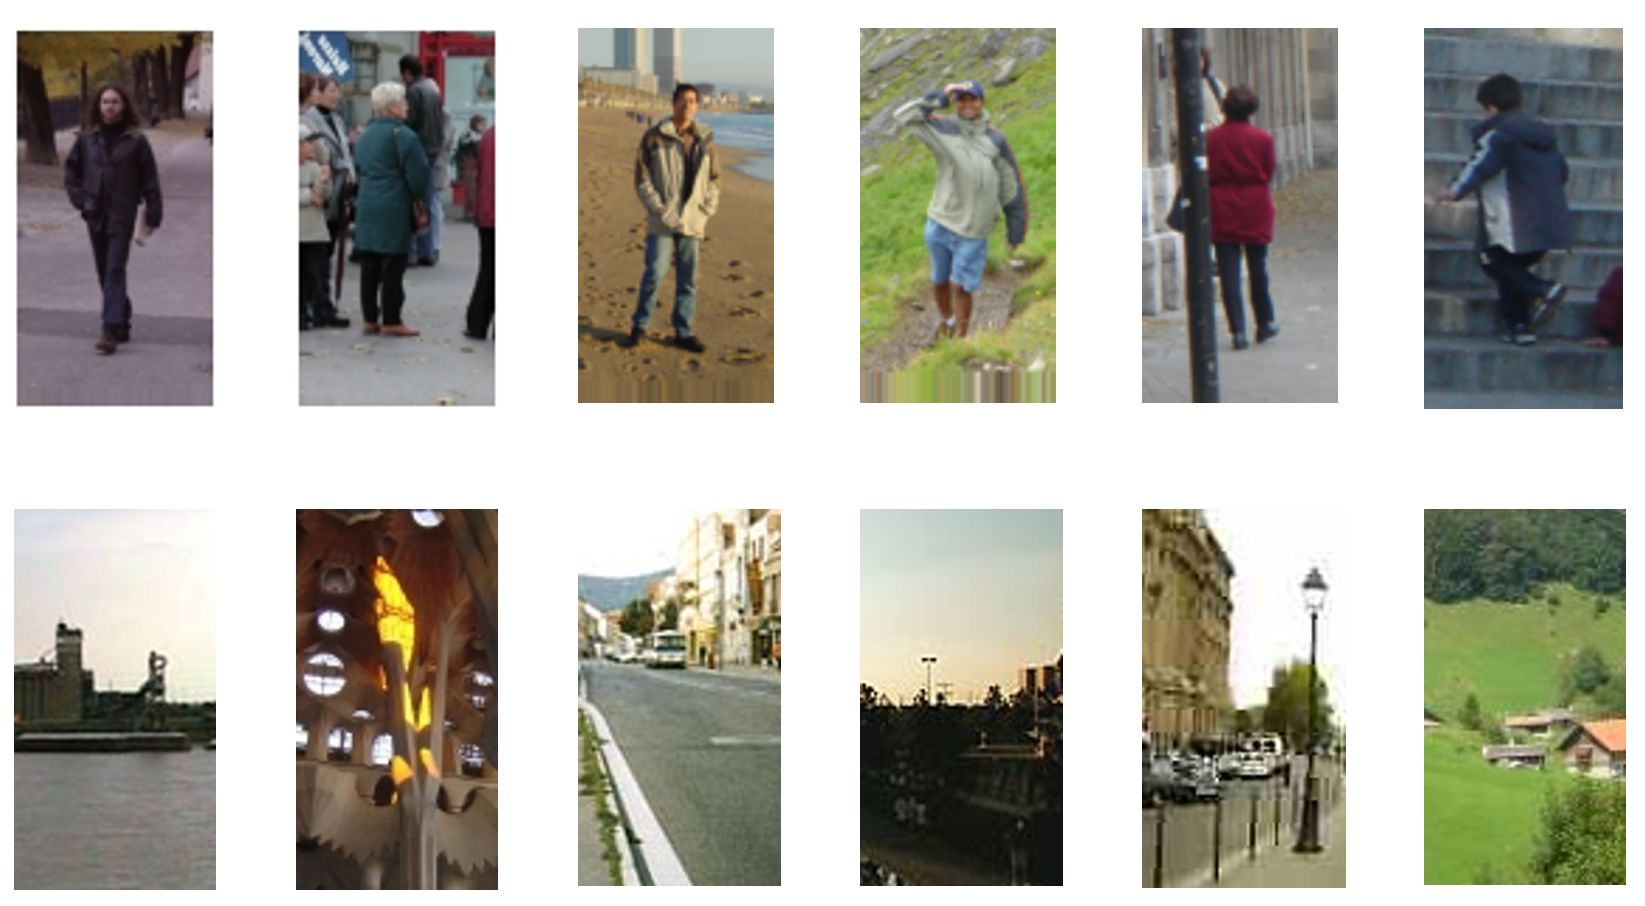
\includegraphics[width=14.5cm]{2_HOG_image_examples.jpg}
	\caption{Przykłady obrazów ze zbioru wykorzystanego przy uczeniu - po lewej dwie próbki pozytywne, po prawej dwie negatywne}
	\label{fig:HOG_image_examples}
\end{figure}
Wśród próbek pozytywnych połowa plików to duplikaty odwrócone horyzontalnie. Ma to zapewnić poprawne uwzględnienie cech usób niezależnie od orientacji względem kamery.

\subsection{Klasyfikacja}
\label{sec:klasyfikacja}
Etap ten jest stosunkowo prosty i stanowi główną zaletę klasyfikatora SVM. Wymaga bowiem wcześniejszego przeprowadzenia etapu uczenia, oraz dostarczenia wektora cech klasyfikowanego obiektu. Realizowane jest wówczas równanie:
\begin{equation}
\label{eq:HOG_classification}
\left.\begin{aligned} 
r=-\sum_{i=1}^{N}a_i(l_i+b_i)-c,
\end{aligned}\right.
\end{equation}
gdzie $a$, $b$ oraz $c$ to parametry hiperpłaszczyzny ($a$ i $b$ - wektory, $c$ - skalar), wszystkie wyliczone na etapie uczenia.
Jeśli $r>0$, detekcja wskazuje obiekt jako przynależący klasy, w przeciwnym wypadku go odrzuca.


\chapter{Implementacja modelu programowego}
Pierwszym zadaniem było stworzenie modeli programowych algorytmów MeanShift oraz Hog+SVM, bez warstwy nadzorującej/sterującej dronem. Wybrano środowisko MATLAB ze względu na jego powszechne zastosowanie w branży naukowej/inżynierskiej, co skutkuje olbrzymią bazą bibliotek i materiałów pomocniczych. W tym przypadku MATLAB ułatwia pracę na obrazach lub sekwencjach wideo poprzez: wczytywanie materiału, wyświetlanie, dostęp do poszczególnych klatek oraz zapewnia wiele wbudowanych funkcji, m.in. do konwersji określonych przestrzeni barw oraz obliczania maszyny wektorów nośnych.

\section{Model MeanShift}

Skrypt rozpoczyna działanie od wyznaczenia jądra obszaru o wymiarach $100 \times 100$ oraz jego gradientów. Po tym następuje właściwa część algorytmu, która pracuje na wczytanym materiale wideo, przekonwertowanym do przestrzeni HSV. Obszarem śledzonym jest kwadrat $100\times 100$, który dla pierwszej klatki obrazu jest zlokalizowany w miejscu startowym ramki $1280\times 720$ pikseli. Dla tego fragmentu obliczany jest histogram barw. Wczytując kolejne klatki, algorytm oblicza histogram kandydatów ostatecznie zestawiając go z oryginalnym i wyznaczając przesunięcie w pionie i poziomie. Dla każdej z klatek operacja ta jest przeprowadzana 10 razy, poprawiając precyzję ostatecznego przesunięcia. Przed rozpoczęciem przetwarzania kolejnej klatki, następuje aktualizacja pozycji obszaru. Po wykonaniu algorytmu dla zdefiniowanej liczbie klatek, skrypt wyświetla film w oryginalnych barwach RGB z dorysowaną czerwoną ramką otaczającą śledzony obszar, co pozwala wizualnie sprawdzić poprawność działania całego kodu. Niestety, czas wykonania tej symulacji jest nieporównywalnie dłuższy od rzeczywistego trwania sekwencji i, przykładowo, na notebooku wyposażonym w procesor klasy i7 materiał o długości XXX jest przetwarzany w czasie ok. 

\section{Model HoG+SVM}

Głównym zadaniem modelu programowego jest próba znalezienia osoby w przeskalowanym obrazie, bazując na obszarze wokół wprowadzonych współrzędnych punktu środkowego.

Działanie skryptu rozpoczyna się od przeprowadzenia sekwencji uczenia klasyfikatora, która bazuje na dwóch tablicach: jedna agreguje wektory cech, a druga przechowuje skojarzone z nimi klasy (0 lub 1). Wykorzystywana baza obrazów wyposażona jest w pliki z ich listami (osobno dla pozytywnych i negatywnych przykładów), co umożliwia proste wczytywanie kolejnych próbek. Oczekuje się tu rozmiaru $128\times 64$ pikseli, jednak niektóre (zwłaszcza negatywne) obrazy są za duże - przeprowadza się tutaj wycięcie fragmentu o podanym wyżej rozmiarze ze środka każdej próbki. Kolejnymi etapami dla takiego obszaru są kolejno: konwersja do odcieni szarości oraz obliczenie wektora cech. Ten proces przeprowadzono zgodnie z informacjami zawartymi w \ref{sec:HOG&SVM}; za normę blokową obrano L2 (\ref{eq:HOG_norm3}), natomiast rozmiar komórki to $4\times 4$ piksele. Po przetworzeniu każdego obrazu dopisuje się wektor cech oraz klasę do odpowiednich tablic.
\newline
Gotowe zestawy danych stanowią parametry dla wbudowanej w MATLABa funkcji \textit{svmtrain}, która zwraca strukturę \textit{svm\char`_struct} z parametrami wykorzystywanymi potem przez klasyfikator.

Opisany powyżej proces ma powtarzalne wyniki, jest jednorazowy, lecz także dość czasochłonny - dlatego nie ma potrzeby przeprowadzać go niepotrzebnie (sprawdzana jest obecność zmiennej \textit{svm\char`_struct}).

Właściwa część skryptu rozpoczyna się od wczytania obrazu wejściowego. O jego odpowiednim przeskalowaniu decyduje parametr ustawiany przed rozpoczęciem działania. W ten sposób zdefiniowane są również współrzędne środka obszaru detekcji. Kolejnym krokiem jest obliczenie $5\times 9$ wektorów cech na fragmencie $144 \times 96$ - widoczna różnica w podejściu względem procesu uczenia wynika z planu znalezienia jak najlepszego wyniku detekcji w danym obszarze. Idąc za przykładem wbudowanej w MATLAB funkcji \textit{svmclassify}, następuje klasyfikacja każdego obliczonego wektora cech. Końcowym etapem jest wyświetlenie przeskalowanego obrazu w kolorze, z naniesionym konturem o wymiarach $128\times 64$ otaczającym obszar najlepszej detekcji.
\chapter{Implementacja sprzętowa systemu wizyjnego}
\section{Układy FPGA}
Najważniejszym i najbardziej czasochłonnym elementem pracy była implementacja algorytmu śledzącego na obiekcie latającym. Obecnie istnieje możliwość skorzystania z przeróżnych cyfrowych jednostek obliczeniowych, które dzieli się, jak przedstawiono poniżej:
\begin{itemize}
	\item brak możliwości zmiany funkcjonalności po wyprodukowaniu układu:
	\begin{itemize}
		\item procesory ASIP (ang. \textit{Application Specific Instruction Set Processor}) - zaprojektowane z dedykowanym zestawem instrukcji		
		\item układy ASIC (ang. \textit{Application Specific Integrated Circuit}) - zaprojektowane do realizacji określonej z góry zadań
		\item procesory ogólnego przeznaczenia CPU (ang. \textit{Central Processing Unit})
		\item procesory graficzne GPU (ang. \textit{Graphics Processing Unit})
		\item procesory sygnałowe DSP (ang. \textit{Digital Signal Processor})
	\end{itemize}
	\item z możliwością konfiguracji po procesie produkcyjnym:
	\begin{itemize} 
		\item układy rekonfigurowalne z architekturą gruboziarnistą
		\item układy rekonfigurowalne z architekturą drobnoziarnistą - FPGA (ang. \textit{Field-Programmable Gate Array}) oraz CPLD (ang. \textit{Complex Programmable Logic Device})
	\end{itemize}
\end{itemize}
Układy ASIC są niestety drogie w prototypowaniu. Procesory CPU nie pozwolą na przetworzenie tak wielkiej ilości danych w czasie rzeczywistym. Z kolei druga grupa urządzeń ma atut polegający na możliwości zmiany architektury układu oraz zrównoleglenia obliczeń tak bardzo, jak tylko pozwala na to ilość dostępnych zasobów. Dodatkowo - i paradoksalnie zarazem - urządzenia te charakteryzują się stosunkowo niskim zapotrzebowaniem na energię. Ma to istotne znaczenie, mając na uwadze światowy trend poszukiwań energooszczędnych rozwiązań w każdej branży. Obszary, w których FPGA znajduje zastosowanie to między innymi:
\begin{itemize}
	\item studia dźwiękowe,
	\item telekomunikacja,
	\item przemysł motoryzacyjny/zbrojeniowy/lotniczy/kosmiczny,
	\item szyfrowanie i przetwarzanie danych,
	\item aparatura medyczna,
	\item systemy wizyjne.
\end{itemize}
To wszystko nie oznacza jednak, że układy FPGA nie są pozbawione wad. Przykładowo, nie można zrealizować na nich niektórych rodzajów algorytmów, głównie rekurencyjnych. Ponadto, sam proces rozwoju konkretnej architektury nie należy do najprostszych i może wymagać potwierdzenia funkcjonalności na kilka sposobów:
\begin{itemize}
	\item porównanie wyników z innym, konwencjonalnym środowiskiem (MATLAB, OpenCV),
	\item symulacja projektu HDL na komputerze,
	\item weryfikacja wybranych sygnałów na układzie przy użyciu zintegrowanego analizatora logicznego (SignalTap dla urządzeń Altery, ILA dla układów Xilinxa).
\end{itemize}
Część problemów bywa z czasem rozwiązywana przez producentów. Stopień skomplikowania projektu można znacznie zredukować, wykorzystując dostępną z oprogramowaniem własność intelektualną - odpowiednio skonfigurowane tzw. IP Core'y - i łącząc sygnały pomiędzy nimi na graficznych diagramach. Co więcej, narzędzie Vivado High-Level Synthesis (HLS) oferuje możliwość adaptacji języka C/C++ do technologii FPGA, upraszczając proces powstawania architektury. \newline Postępująca zwłaszcza w ostatnich latach integracja i zmniejszanie procesu technologicznego pozwoliły na stworzenie układów łączących logikę programowalną (FPGA) oraz dwurdzeniowy procesor ARM. Krzem, na którym oprócz jednostki obliczeniowej znajdują się różne peryferia, nosi nazwę układu heterogenicznego, w branży bardziej znanego jako \textit{System on a Chip} (SoC). Dzięki magistrali (przykładowo AXI) zapewniającej szybką wymianę danych pomiędzy blokami, taki układ pozwala łączyć możliwość zrównoleglania obliczeń, którą daje logika programowalna (\textit{ang. PL - Programmable Logic}), oraz prostotę rozwoju oprogramowania uruchamianego na procesorze (\textit{ang. PS - Processing System}). W tej ostatniej części istnieje możliwość uruchomienia systemu operacyjnego (jednej ze specjalnych dystrybucji Linuxowych) lub nawet stworzenia konfiguracji opartej o wieloprocesorowość asynchroniczną (ang. AMP). Warto tu zauważyć, że narzędzia syntezy logiki od dawna oferowały możliwość stworzenia softprocesorów w układach FPGA (Altera - Nios, Xilinx - MicroBlaze), jednak te rozwiązania istotnie ograniczały dostępne zasoby, a częstotliwość taktowania takich komponentów rzadko przekraczała 200 MHz. \newline

Powyższa charakterystyka przekonuje, że układy FPGA, a zwłaszcza SoC mógłby być szczególnie doceniony na platformie latającej, gdyż byłby w stanie sprostać wymaganiom stawianym przez zadanie przetwarzania obrazu w czasie rzeczywistym, a dzięki niewielkim wymiarom i niskiemu zużyciu energii nie stanowiłby wielkiego obciążenia przy i tak już mocno ograniczonym czasie lotu na jednej baterii. \newline
Ze względu na charakter pracy użyto w niej układu ZYNQ SoC firmy Xilinx. Oczywiście, ze względu na poziom skomplikowania montażu tego urządzenia nie podjęto decyzji o prototypowaniu własnego obwodu drukowanego, lecz wykorzystano niewielki, lecz bogaty w peryferia zestaw PYNQ z układem ZYNQ SoC XC7Z020. Oprogramowaniem wspierającym rozwój architektury na to urządzenie jest pakiet Xilinx Vivado + SDK.

\section{Tor wizyjny w układzie FPGA}
\label{sec:counter}
Stworzony system wizyjny jest złożonym drzewem zależności pomiędzy wieloma modułami. By jednak był on torem wizyjnym, konieczne jest odebranie sygnału wideo z zewnątrz - w tym wypadku poprzez port HDMI - i poprawne zdekodowanie go do podstawowej, użytecznej przestrzeni barw RGB. Taki zestaw sygnałów jest dość prosty do uwzględnienia w tworzonych algorytmach. Opcjonalne i zalecane jest również wyprowadzenie przetworzonego sygnału RGB na monitor, który pozwoli zweryfikować poprawność tworzonej architektury. Wyżej opisany szkielet został stworzony w tzw. Block Designie, a poza modułami firmy Xilinx wykorzystano konwertery DVI$\rightarrow$RGB oraz RGB$\rightarrow$DVI dostarczone przez firmę Digilent - producenta zestawu PYNQ. Dodatkowo, podstawowym źródłem taktowania został dostarczany z karty PYNQ zegar o częstotliwości $125$MHz oraz sygnał inicjujący działanie algorytmu, pochodzący z odbiornika radiowego.

 

Sygnały wideo, które można wyodrębnić po zdekodowaniu, to:
\begin{itemize}
	\item zegar taktujący pikseli ($74.25$MHz)
	\item kolor czerwony R (8 bitów),
	\item kolor zielony G (8 bitów),
	\item kolor niebieski B (8 bitów),
	\item synchronizacja pozioma - poziom wysoki sygnalizuje koniec poziomej linii,
	\item synchronizacja pionowa - poziom wysoki sygnalizuje koniec klatki obrazu,
	\item sygnał aktywny - poziom wysoki sygnalizuje obecność poprawnego piksela.
\end{itemize}
Z góry założono, że transmisja i przetwarzanie wideo będzie się odbywać w oparciu o standard \textit{720p/60fps}. Uwzględniając narzut dany przez sygnały sterujące, ostateczna częstotliwość taktowania piksela wynosi w tym przypadku $74.25$MHz. To właśnie ten zegar, nazywany dalej w pracy \textit{\boldmath pixel\char`_clk}, stanowi podstawę potokowego przetwarzania obrazów w układzie FPGA. Poniższa ilustracja przedstawia zapis klatki z sygnałami sterującymi, gdzie jednostką jest cykl zegara taktującego piksel. 

\begin{figure}[h]
	\centering
	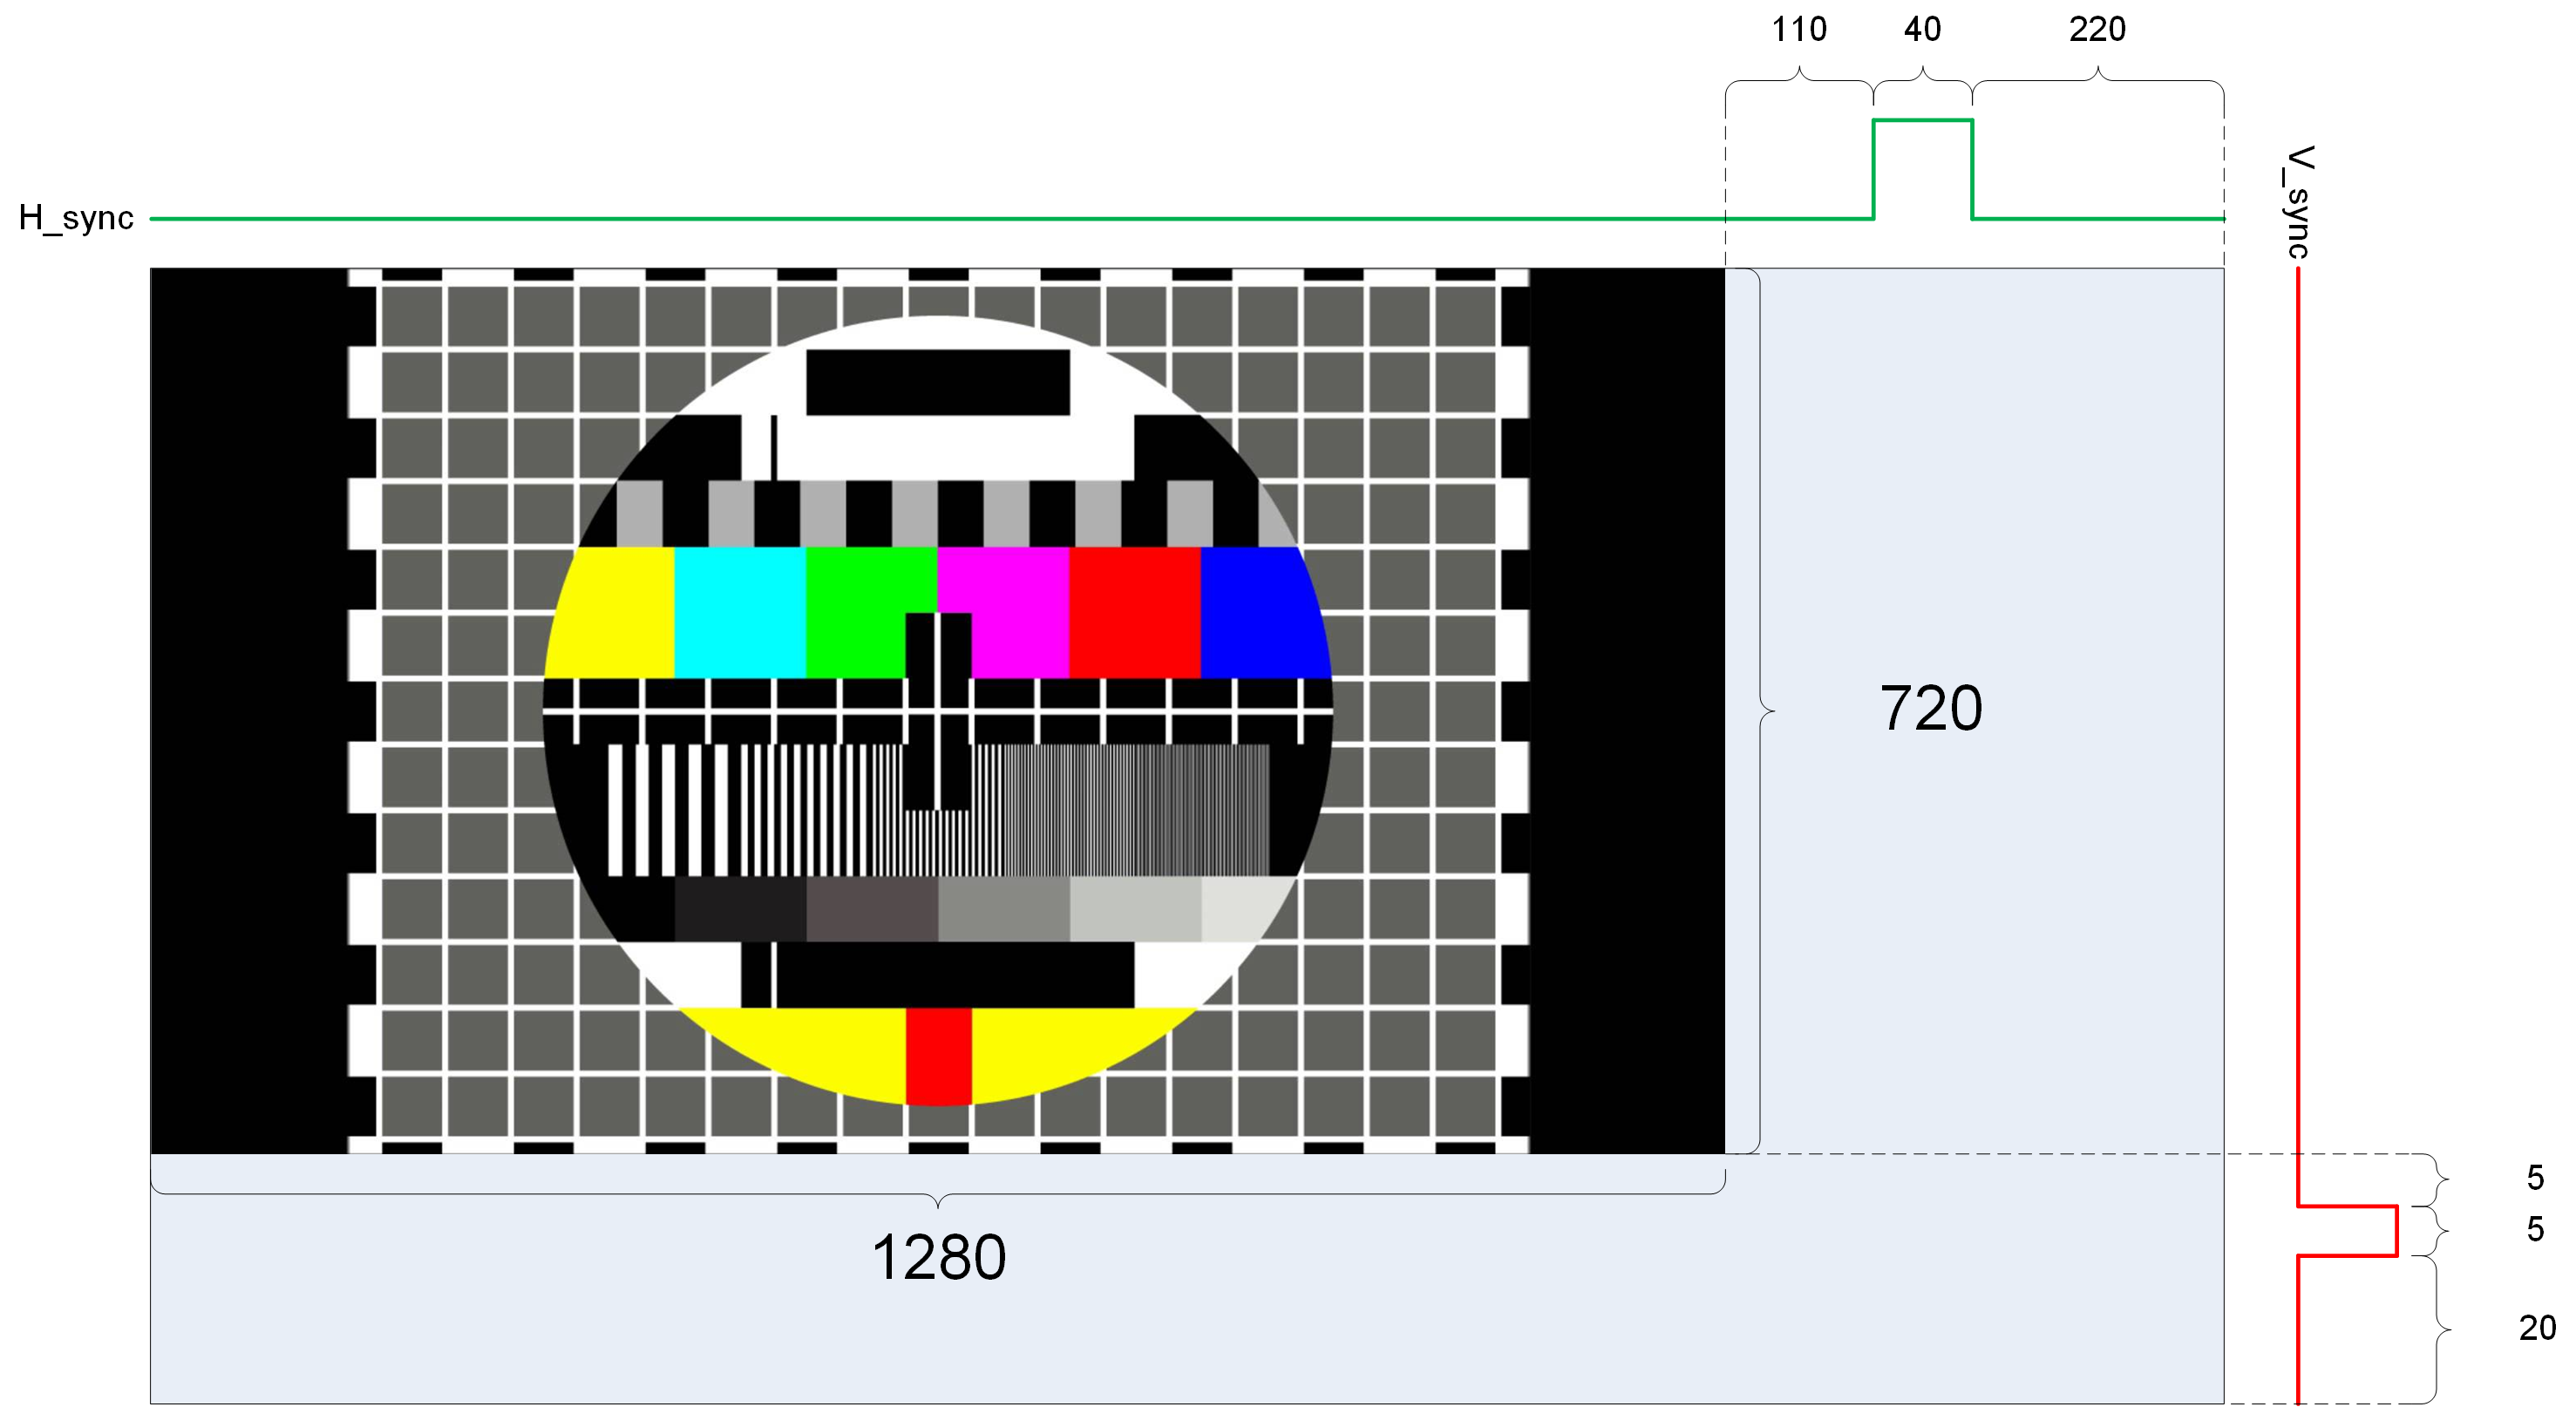
\includegraphics[width=17cm]{4_720p.png}
	\caption{Schemat zapisu klatki w rozdzielczości $720p$}
	\label{fig:720_frame}
\end{figure}

Algorytmy opisane w dalszej części pracy będą często posiłkować się informacją o aktualnym położeniu piksela na właściwym obrazie. Stworzono w tym celu licznik kalkulujący tę pozycję dla osi pionowej i poziomej w oparciu o długości trwania sygnałów kontrolnych z rysunku \ref{fig:720_frame}. 

 
\section{Realizacja algorytmu MeanShift}
Bazą do pracy nad implementacją było określenie wielkości obszaru śledzonego. Uwzględniając parametry optyczne kamery, jak i rozdzielczość wejściową materiału wideo podjęto decyzję o śledzeniu obszaru o wymiarach $100 \times 100$ pikseli. Analizując możliwości pracy układu okazało się, że algorytm jest w stanie przetwarzać każdą otrzymaną klatkę (lub raczej jej określony fragment) - częstotliwość jego pracy wynosi zatem \textit{60Hz}.\newline
Wstępnym etapem na drodze danych w algorytmie MeanShift jest konwersja przestrzeni barw, realizowana zgodnie ze wzorami \ref{HSV_first}-\ref{HSV_last} w module \textit{rgb2hsv}. Moduł działa w trybie potokowym pracując na zegarze \textit{pixel\char`_clk} i odpowiednio opóźnia wszystkie sygnały sterujące, co jest istotnym warunkiem poprawnego rozpoznawania odpowiednich pikseli w dalszych etapach przetwarzania.
Dane te są na bieżąco dostarczane do modułu \textit{Meanshift}, realizującego główną część zadań. 

\subsection{Inicjalizacja}
Mimo, że właściwe działanie algorytmu ma miejsce po otrzymaniu sygnału zewnętrznego (\textit{algorithm\char`_en}), wymaga on wcześniejszej inicjalizacji - odbywa się ona tuż po zaprogramowaniu układu FPGA. W głównej mierze jest ona związana z obliczeniem jądra i jego gradientów. Dane te, wykorzystywane potem w charakterze informacji tylko do odczytu, muszą tu być zapisane w dość uporządkowany sposób. Najlepiej nadaje się do tego konfigurowalna pamięć BRAM. Powinna ona przechowywać informacje dla wszystkich elementów obszaru, to jest 10000 pól. Jej ostateczną organizację przedstawia tabela \ref{tab:kerBRAM}. 
\newcolumntype{P}[1]{>{\centering\arraybackslash}p{#1}}
\begin{table}[h]
\centering
\begin{tabular}{|P{5cm} |P{3cm} |P{2.5cm}|}

\hline
\rowcolor{lightgray} Informacja & Adres rejestru & Format \\ 
Jądro: $K(||P-P'(x,y)||)$				& 0:9999		& U3.15\\ 
\hline
Gradienty: $g_x$, $g_y$		& 10000:19999	& S0.11, S0.11\\ 
\hline
Norma: $\sqrt{g_x^2+g_y^2}$	& 20000:29999	& U0.11\\ \hline
\end{tabular}
\caption{Organizacja pamięci BRAM \textit{kernel\char`_ram}}
\label{tab:kerBRAM}
\end{table}
\newline
Warto nadmienić, że zestaw informacji związanych z konkretnym pikselem w obszarze 100x100 opisują rejestry pod adresami:
\begin{equation}
\{100y+x, 10000+100y+x, 20000+100y+x\}, x,y=0..99,
\end{equation}
umożliwiając czytelny i sprawny dostęp do tych danych. By umożliwić odczyt obydwu gradientów w jednym cyklu zegara, zagregowano je w wektor o długości rejestru, tj. 18 bitów. Obserwacje poczynione na zapisie gradientów w symulacji dowiodły jednak, że  3 najstarsze bity ułamkowe są zawsze równe bitowi znaku. Można zatem rozszerzyć precyzję informacji o gradiencie, zapisując ją w rejestrze w notacji S0.11, a nie S0.8 - co pozytywnie wpływa do dokładność obliczeń. \newline
Po zapisaniu wartości do kompletu rejestrów ustawiana jest flaga \textit{kernel\char`_rom\char`_ready}, której obecność sygnalizuje gotowość uruchomienia właściwej części algorytmu. Jak stwierdzono w oparciu o symulacje, w rzeczywistości inicjalizacja pamięci \textit{kernel\char`_rom} trwa około 5ms, jest to zatem pomijalnie krótki czas, niewpływający na funkcjonalność (<1 klatka obrazu).

\subsection{Zapis obszaru wideo}
\label{ssec:savideo}
Na szerszy opis zasługuje sposób zapisu informacji z obrazu, należy bowiem tymczasowo zapamiętać wartości pikseli $H$, na których obliczenia będą kilkukrotnie wykonywane. Dużym obciążeniem dla zasobów układu byłaby próba zapisania całych klatek - pojedyncza wymagałaby: $1280\cdot720\cdot9\text{b} = 1.037$MB dostępnego miejsca. Z tego względu postanowiono zapisywać jedynie obszar w aktualnym położeniu obiektu, z dodatkowym sąsiedztwiem 15 pikseli z każdej strony oraz uwzględniając w tej procedurze zabezpieczenie na wypadek próby wyjścia poza przestrzeń obrazu. Sąsiedztwo to pozwoli algorytmowi wskazać przesunięcie obszaru najbardziej zbliżone do faktycznego ruchu obiektu. Szerokość paska sąsiedztwa - 15 pikseli - dobrano metodą doświadczalną, uwzględniając maksymalne przemieszczenia obiektu pomiędzy kolejnymi klatkami.

Proces śledzenia  musi poprawnie określić położenie aktualnego, \enquote{użytecznego} piksela, a także rozpoznać początek kolejnej klatki. Jest to możliwe poprzez stworzenie logiki opierającej się na licznikach: horyzontalnym i wertykalnym, analizującą zbocza sygnałów sterujących. Liczniki wykorzystują informacje przedstawione na rysunku \ref{fig:720_frame}; zliczają odpowiednio do wartości 1280 oraz 720.

Otrzymanie sygnału \textit{algorithm\char`_en} inicjuje realizację algorytmu. Istotne jest, aby w momencie pojawienia się tego sygnału, w obszarze zdefiniowanym jako startowy (domyślnie środek obrazu) znajdował się śledzony obiekt. Obszar ten, będący od teraz wzorcem, jest zatrzaskiwany na najbliższej pełnej klatce obrazu. Następnie obliczana jest funkcja gęstości prawdopodobieństwa, opisana w sekcji \ref{ssec:fgp}.

Wartości pikseli - linia po linii -  są przechowywane w module BRAM działającym w trybie True Dual Port, \textit{image\char`_data\char`_ram}. Dzięki temu możliwy jest jednoczesny zapis/odczyt pod warunkiem, że porty nie pracują jednocześnie na tym samym adresie. Ze względu na konieczność posiadania kompletnego fragmentu obszaru i możliwość zapisu kolejnego, pamięć zdolna jest pomieścić 2 obszary z ostatnich klatek, każdy o wymiarach $130 \times 130$: łącznie 33800 adresów. Zamiennie, co klatkę, wykonywany jest zapis najnowszych danych do jednej połowy przestrzeni, i przetwarzanie (odczyt) drugiej. Warto jednak zwrócić uwagę na rozbieżność w szybkości obu tych procesów -  o ile dane zapis działa synchronicznie z zegarem piksela, \textit{pixel\char`_clk}, to algorytm będzie odczytywał dane z prędkością \textit{\boldmath calc\char`_clk}, celowo taktowanego innym zegarem (100MHz).
\newcolumntype{P}[1]{>{\centering\arraybackslash}p{#1}}
\begin{table}[h]
	\centering
	\begin{tabular}{|P{4cm} |P{3cm} |P{2cm}|}
		
		\hline
		\rowcolor{lightgray} Informacja & Adres rejestru & Format \\ 
		Klatka $t\%2==0$			& 0:16899		& U9\\ 
		\hline
		Klatka $t\%2==1$		& 16900:33799	& U9\\ 
		\hline
	\end{tabular}
	\caption{Organizacja pamięci BRAM \textit{image\char`_data\char`_ram}}
	\label{tab:imageBRAM}
\end{table}
\newline

\subsection{Funkcja gęstości prawdopodobieństwa}
\label{ssec:fgp}
Wartość funkcji gęstości prawdopodobieństwa jest inaczej wartością histogramu dla danej barwy piksela ($H$ z zakresu 0-359). W tym celu utworzono pamięć BRAM, która przechowuje dwa histogramy dla wzorca oraz kandydata - w sumie 720 rejestrów. 
\newcolumntype{P}[1]{>{\centering\arraybackslash}p{#1}}
\begin{table}[h]
	\centering
	\begin{tabular}{|P{4cm} |P{3cm} |P{2cm}|}
		
		\hline
		\rowcolor{lightgray} Informacja & Adres rejestru & Format \\ 
		Histogram wzorca			& 0:359		& U10.15\\ 
		\hline
		Histogram kandydata		& 360:719	& U10.15\\ 
		\hline
	\end{tabular}
	\caption{Organizacja pamięci BRAM \textit{histogram\char`_ram}}
	\label{tab:histBRAM}
\end{table}
\newline
Histogram wzorca jest tworzony raz, w oparciu o pierwszy obraz; kolejne histogramy dotyczą już kandydata i zostają zapisane w górnej połowie adresowej (H+360). Piksel, uzyskując dostęp do odpowiedniego rejestru, dodaje wartość jądra odpowiadającą jego pozycji na obszarze $100 \times 100$, tworząc ostatecznie funkcję gęstości prawdopodobieństwa. Format rejestrów pamięci \textit{histogram\char`_ram} pozwala na zapis wartości o zakresie [0:1023.99997].
Zdarzają się jednak przypadki, gdy większość pikseli na obszarze (zwłaszcza w centrum - miejscu największych wartości jądra) jest jednokolorowa, co może skutkować próbą przekroczenia dopuszczalnych wartości dla rejestru. Chroni przed tym dodatkowy fragment logiki, który wykrywając takie zdarzenie, pozostawia rejestr z maksymalną wartością.

Wartość pikseli odczytuje się bezpośrednio z pamięci przechowującej analizowany obszar, opisanej w \ref{ssec:savideo}. Zliczające na bieżąco (do 100) rejestry \textit{H\char`_count} oraz \textit{W\char`_count} obliczają pozycję aktualnie odczytywanego piksela, w odniesieniu do lewego górnego rogu. Nie jest to jednak swobodna inkrementacja i wykorzystanie każdego piksela z pamięci - w zachowanym obszarze przechowuje się również piksele z sąsiedztwa. Bazując na wartościach \textit{offset\char`_X} oraz \textit{offset\char`_Y}, pozwala się wybrać tylko 100 określonych pikseli ze 100 określonych linii. Przykładowo, obliczając po raz pierwszy histogram dla ostatnio zapisanej klatki zmienne \textit{offset\char`_X} i \textit{offset\char`_Y} mają wartości domyślne $(15,15)$. Oznacza to, że z zapisanego obszaru o wymiarach $130\times 130$ należy wybrać fragment, którego pierwszym pikselem w lewym górnym rogu będzie ten o indeksie $(15,15)$. Zakres dopuszczalnych wartości dla każdej z tych zmiennych to $<0,29>$.

Po przejściu przez wszystkie piksele obszaru następuje ustawienie flagi \textit{histogram\char`_ready}, gdzie w przypadku przetwarzania klatki-wzorca algorytm przechodzi do akwizycji pierwszego kandydata, natomiast dla każdej kolejnej rozpocznie obliczanie funkcji podobieństwa.
Podobnie jak \textit{image\char`_data\char`_ram}, \textit{histogram\char`_ram} działa w trybie True Dual Port. Po obliczeniu funkcji gęstości dla aktualnego obszaru jest on w stanie jednocześnie odczytywać wartości funkcji dla wzorca i kandydata, umożliwiając wykonywanie części dalszych obliczeń w sposób równoległy.

\subsection{Funkcja podobieństwa}
Moduł implementujący kalkulację funkcji podobieństwa (i ostatecznie przesunięcia) obszaru, jest najbardziej złożony w tej części systemu. Funkcja podobieństwa, opisana wzorem \ref{eq:position}, jest obliczana na każdym pikselu w pamięci należącym do właściwego obszaru (bez sąsiedztwa).

Dla każdego piksela z obszaru $100 \times 100$, będącego adresem dla pamięci $histogram\char`_ram$, wczytywana jest wartość funkcji prawdopodobieństwa wzorca i kandydata. Moduł oblicza ich iloraz (wzorzec/kandydat) używając odpowiedniego bloku dostarczonego przez firmę Xilinx. Ze względów optymalizacyjnych obcięto 9 najmłodszych bitów obu wartości, gdyż nie wpływały w większym stopniu na dokładność, a ich pozbycie pozwoliło zmniejszyć latencję modułu. Podczas takiego dzielenia logika musi ponadto sprawdzić obecność zera w mianowniku - wówczas iloraz powinien być zerowany. Brak obsługi takiego zdarzenia doprowadziłby do otrzymania ilorazu o trudnej do przewidzenia wartości - mogłoby to powodować poważne błędy w działaniu algorytmu. 

Gotowy iloraz należy poddać pierwiastkowaniu. Moduł obliczający pierwiastek wymaga, by wejście z danymi było liczbą całkowitą, lub  też ułamkową - ale z jednym bitem dla części całkowitej: U1.X. W tym celu wynik dzielenia - liczba w formacie: U16.16 - została obcięta do U13.11., a następnie "wirtualnie" przesunięta o 12 bitów w prawo, do postaci: U1.23. Wynik pierwiastkowania wymaga przesunięcia w lewo już tylko o 6 bitów ($\sqrt{2^{12}}=2^6$), po czym jest obcinany do 16 najbardziej znaczących bitów: U7.9.
Operacje te, mimo że zawiłe, nie wpływają na wynik, lecz gwarantują poprawne działanie modułu \textit{CORDIC} realizującego pierwiastkowanie.

Wartości pierwiastka współtworzyć będą zarówno licznik, jak i mianownik ilorazu wektora MeanShift - rozdzielnie dla przesunięcia pionowego i poziomego. Obliczenie iloczynów wymaga pobrania z pamięci \textit{kernel\char`_ram} obu gradientów oraz ich normy. Odczyt jest zoptymalizowany pod zminimalizowanie liczby cykli zegara potrzebnych na odczytanie obu wartości i został oparty o maszynę stanu, będącą zresztą szkieletem całej tej części algorytmu (OPISAĆ).


\section{Realizacja algorytmu HOG+SVM}

Wymagania stawiane przez system mówią o konieczności rozpoznania osoby wraz z dodatkowym określeniem jej wielkości na ekranie (skala ta pozwoli dość ogólnie wyznaczyć odległość drona od obiektu, co wpłynie na sterowanie maszyny). Z tego względu implementacja musi wykorzystać tzw. piramidę skal, czyli równoległą detekcję HOG+SVM na kilku wielkościach obrazów. Dysponując obrazem o rozdzielczości $1280 \times720$, należy przeskalować go do kilku mniejszych ,a następnie przeprowadzić na nich opisane wcześniej operacje wyliczenia wektora cech, i sklasyfikować przy użyciu SVM. Odpowiednia lokalizacja postaci (i jej odległość od kamery) zostanie wybrana na podstawie najlepszego \textbf{pozytywnego} wyniku klasyfikacji, w oparciu o wartość $r$.\newline
Taki algorytm może rozpocząć działanie jedynie na pełnej klatce obrazu, zatem stworzono mechanizm, który mimo obecności sygnału wyzwalającego pracę algorytmu pozwoli mu pracować dopiero na zboczu opadającym sygnału synchronizacji pionowej. Drugim warunkiem jest to, by w momencie nadejścia nowej klatki algorytm nie był w trakcie przetwarzania poprzedniej - w przeciwnym wypadku histogramy mogłyby być nadpisywane nowymi wartościami. Oznacza to jednak, że co druga klatka obrazu będzie pomijana w przetwarzaniu, ograniczając częstotliwość pracy algorytmu do \textit{30Hz}.

W pierwszej kolejności obraz wejściowy poddawany jest konwersji do skali odcieni szarości. Następna w kolei, operacja skalowania do 5 mniejszych obrazów, jest realizowana na bieżąco, dzięki czemu można zachować sygnały kontrolne VGA (synchronizację poziomą oraz pionową). Na pomniejszonych obrazach obliczane są wektory cech, bazując na komórkach o wielkości $4\times 4$, i blokach o rozmiarze $2\times2$. Nie jest możliwa analiza całego obrazu, a jedynie otoczenia aktualnie śledzonego fragmentu. Musi ono być jednak wystarczająco duże, by klasyfikator miał szansę wybrać jak najlepszą detekcję osoby w jego wnętrzu. Jak wspomniano wcześniej, wektor cech tworzony jest na wycinku o rozmiarze $128\times 64$ pikseli. Obrazuje to poniższy zrzut, gdzie taki wycinek zaznaczono zieloną linią.
\begin{figure}[h]
	\centering
	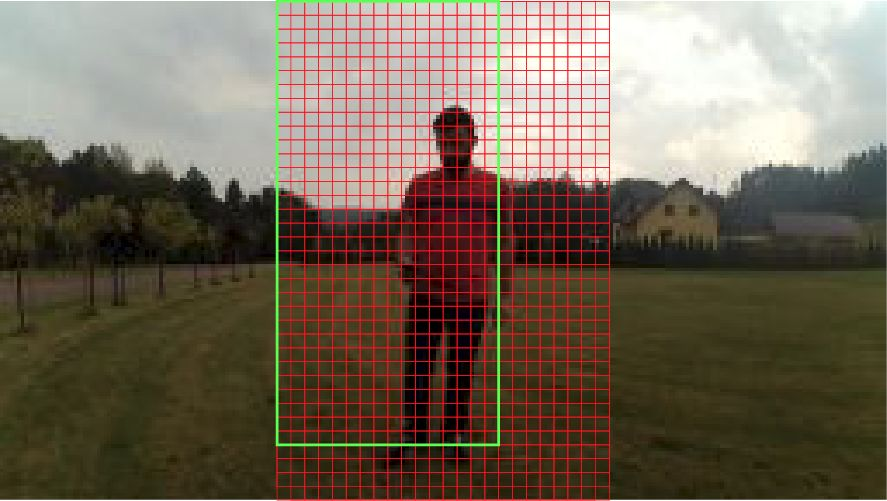
\includegraphics[width=15cm]{4_scaled_hog_example.jpg}
	\caption{Analiza obrazu o rozmiarach $144\times 256$}
	\label{fig:HOG_mesh}
\end{figure}
\newline
Jeśli algorytm będzie pracował na obszarze $144\times 96$, to zakładając stałe położenie komórek na obrazie (są to kwadraty $4\times4$ wydzielone czerwonymi liniami), powstanie łącznie $5\cdot9=45$ wektorów cech. Reszta obrazu zostaje zignorowana. Koordynaty centrum obszaru detekcji są określane na początku działania pojedynczej iteracji algorytmu i są natychmiastowo konwertowane do odpowiednich skal obrazu.

\subsection{Konwersja RGB do skali odcieni szarości}
Obraz wejściowy jest poddawany konwersji zgodnie ze wzorem \ref{eq:rgb2gray}. Używane są tu trzy równoległe mnożarki, a suma iloczynów jest zaokrąglana do 8 bitów (do postaci liczby całkowitej z zakresu 0-255).

\subsection{Skalowanie}
Kolejny etap to przeskalowanie obrazu wejściowego. Sama idea okazuje się być tym bardziej na miejscu, jeśli wziąć pod uwagę parametry kamery zamontowanej na dronie - w przypadku tego projektu jest to Xiaomi Yi, urządzenie do zastosowań sportowych, wyposażone w duży kąt widzenia - 155$^{\circ}$. W efekcie osoba oddalająca się od kamery bardzo szybko zmniejszy swoje wymiary na obrazie. Materiał $720\times 1280$ pikseli przeskalowano do 5 obrazów przy użyciu następujących skal:
\NumTabs{15}
\begin{itemize}
	\item \textbf{1:  2}\tab{:}\tab{$720\times 1280\rightarrow360\times 640$} pikseli
	\item \textbf{1:2.5}\tab{:}\tab{$720\times 1280\rightarrow288\times 512$} pikseli	
	\item \textbf{1:  3}\tab{:}\tab{$720\times 1280\rightarrow240\times 426$} pikseli
	\item \textbf{1:3.5}\tab{:}\tab{$720\times 1280\rightarrow205\times 365$} pikseli
	\item \textbf{1:  4}\tab{:}\tab{$720\times 1280\rightarrow180\times 320$} pikseli
\end{itemize}
Powyższe wartości pozwalają jednocześnie zachować prostotę implementacji (skale są reprezentowane w formacie U3.1) i wyraźnie określić odległość drona od postaci. 

Skalowanie przebiega w dość prosty sposób i polega na pomijaniu nieodpowiednich wierszy lub/i kolumn oryginalnego obrazu. Jeśli założyć, że:
\begin{itemize}
	\item $x_i$, $y_i$ - współrzędne obrazu wejściowego,
	\item $x_o$, $y_o$ - współrzędne obrazu wyjściowego (przeskalowanego),
	\item $s_c$ - skala do zastosowania w pionie oraz w poziomie,
\end{itemize}
to przypisanie wartości obrazu wejściowego nastąpi przy jednoczesnym spełnieniu obu poniższych warunków:
\begin{equation}
\label{eq:scaling}
\left.\begin{aligned} 
x_i&==\lfloor s_cx_o\rfloor \\ 
y_i&==\lfloor s_cy_o \rfloor
\end{aligned}\right.
\end{equation}
Po natrafieniu na odpowiedni piksel, oprócz przypisania jego wartości do wyjścia, wystawiony zostanie sygnał sterujący \textit{valid}, bardzo ważny dla dalszej części algorytmu.
Przykład dla kilku pierwszych wartości \textit{x\char`_o} jest widoczny w tabeli \ref{tab:scaling}.
\begin{table}[h]
	\centering
	\captionsetup{justification=centering,margin=1cm}
	\begin{tabular}{|P{2cm} |P{3cm} |P{2cm}|}	
		\hline
		\rowcolor{lightgray} $x_o$ & $x_is_c$ & $x_i$ \\ 
		1		& 2.5	& 2\\ 
		\hline
		2		& 5		& 5\\ 
		\hline
		3		& 7.5	& 7\\ 
		\hline
		4		& 10	& 10\\ 
		\hline		
	\end{tabular}
	\caption{Przykładowy przebieg skalowania dla $s_c=2.5$ wraz z przypisywanymi pikselami wejściowymi}
	\label{tab:scaling}
\end{table}

Działanie modułu opiera się na stworzeniu dwóch zestawów liczników dla każdej skali. Pierwszy zestawpozwala na zdeterminowanie indeksów piksela wejściowego ($x_i$, $y_i$) i został opisany w sekcji: \ref{sec:counter}. \newline
Drugi zestaw liczników działa zgodnie z poniższym schematem.
\begin{figure}[!h]
	\centering
	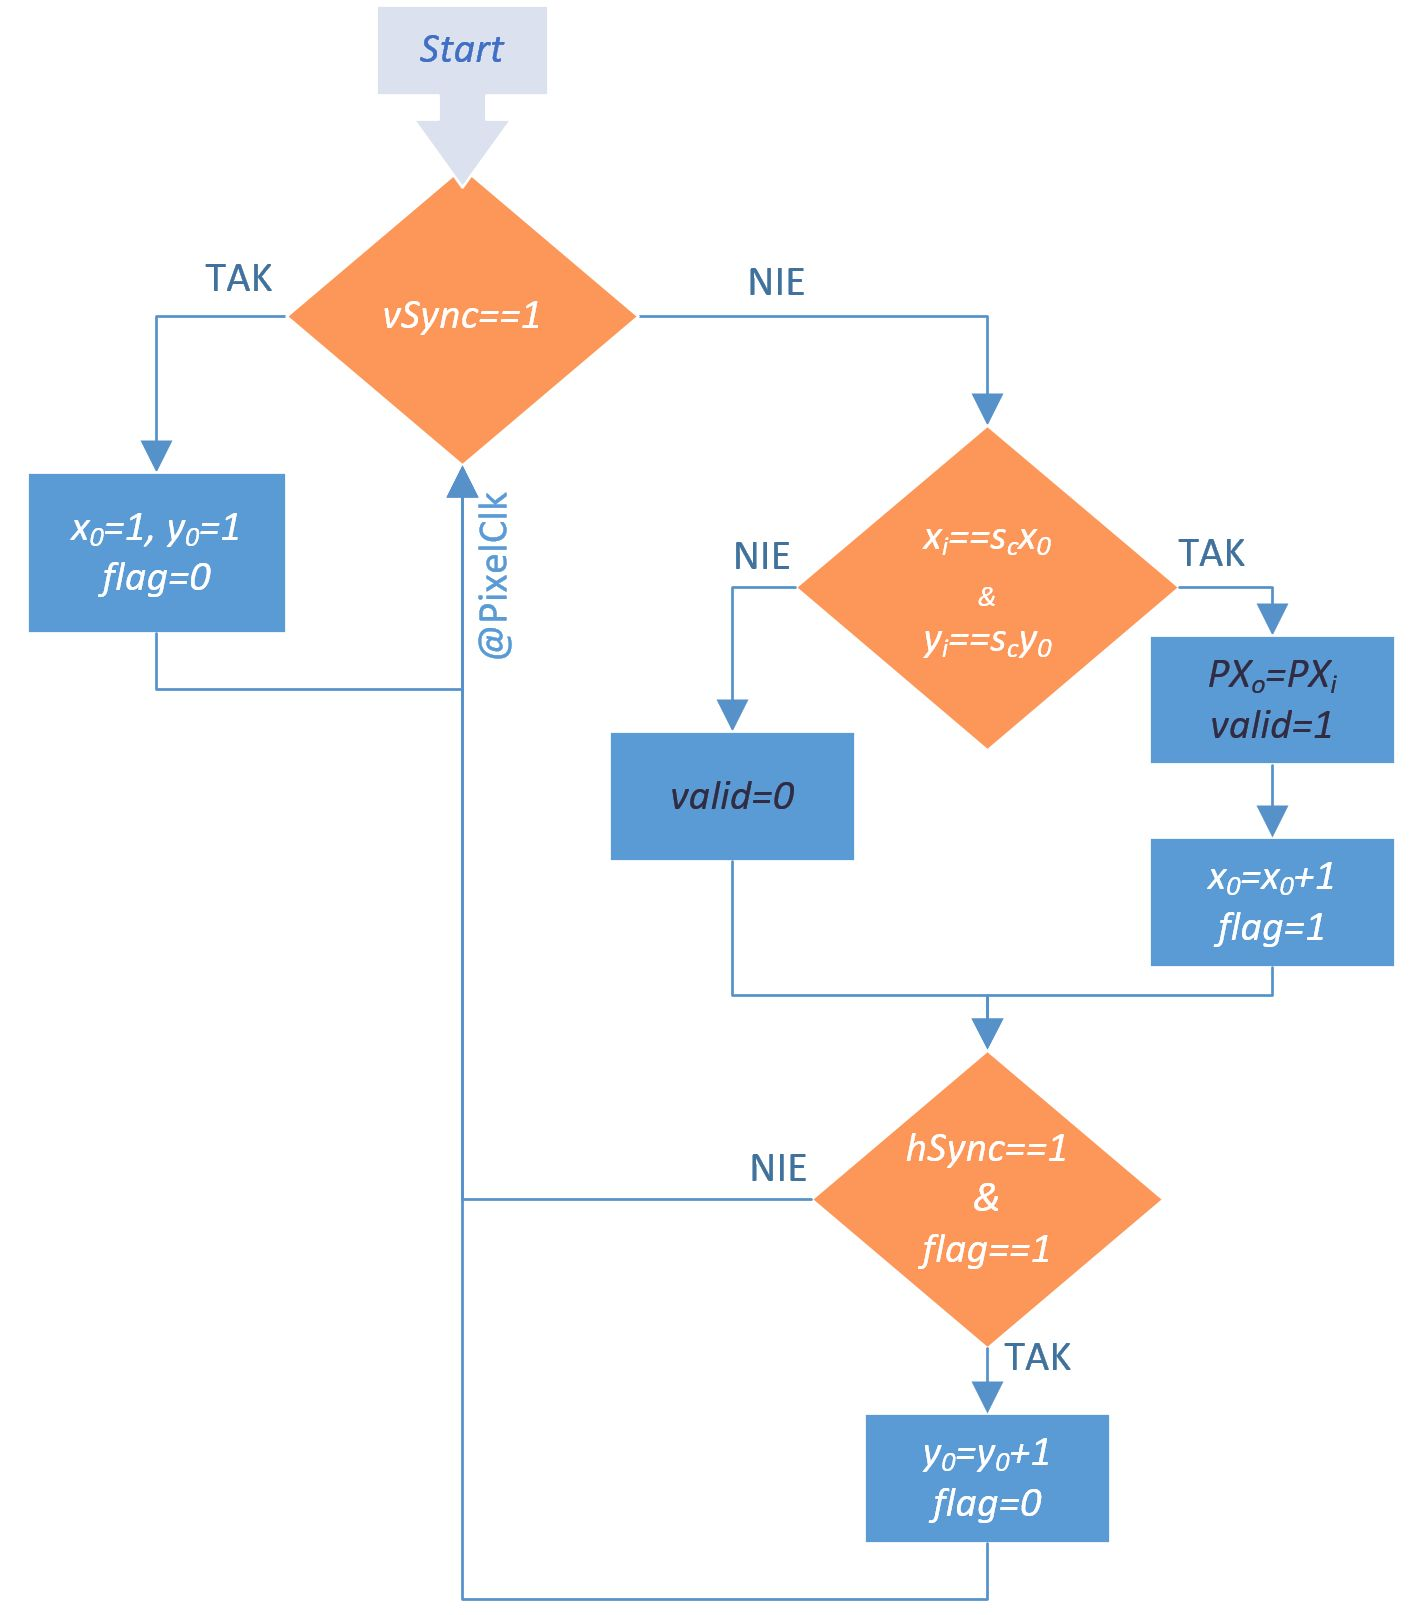
\includegraphics[width=11cm]{4_scaling.jpg}
	\caption{Schemat działania licznika skalującego}
	\label{fig:scaling_sch}
\end{figure}
Oznaczeniem \textit{@PixelClk} opisano proces oczekiwania na kolejne zbocze narastające zegara pikselowego. Gwarancją poprawnie przeprowadzonego procesu skalowania jest obecność sygnałów sterujących VGA - tylko wtedy następuje poprawny przyrost wartości liczników. Z kolei inicjalizacja (po lewej stronie diagramu) ma miejsce po otrzymaniu sygnału synchronizacji pionowej, zatem podłączony do układu sygnał wideo będzie skalowany już od pierwszej pełnej klatki.

\subsection{Obliczanie gradientów}
Nawet odpowiednio przeskalowane obrazy są zbyt duże, by przechowywać informację o ich gradientach. Nie ma jednak takiej potrzeby, jeśli postawi się na implementację algorytmu z maksymalizacją przetwarzania potokowego, opartego o sygnał aktywnego piksela \textit{valid} z modułu skalowania.

Implementacja gradientu pionowego jest nieco złożona, gdyż wymagane w pojedynczej operacji piksele leżą w kilku kolejnych liniach obrazu. Konieczne jest zapamiętanie dwóch ostatnich linii - zrealizowano to przy użyciu dwóch kolejek FIFO. Jedna z nich (oznaczona numerem \#1) rozpoczyna działanie już przy pierwszej linii obrazu i jej zadaniem jest przyjęcie aktualnych pikseli. Kolejka (\#2) przejmie je w kolejnej linii obrazu, gdy (\#1) pozbywając się starych pikseli „wymieni je” na te najnowsze - które wizualnie znajdują sie dokładnie pod nimi na obrazie. Logika została zaprojektowana w sposób pozwalający uzyskać jednoczesny dostęp do 3 kolejnych pikseli leżących w linii pionowej. Duża w tym zasługa specjalnego trybu modułu FIFO - First Word Fall Through (FWFT), dzięki któremu pierwsze dostępne słowo jest natychmiastowo wystawiane na wyjście, i tylko zdejmowane (zastępowane kolejnym) w odpowiedzi na wysoki stan sygnału odczytu.
Ostatecznie algorytm, będąc w linii $i$ ($i>1$), obliczy gradient pionowy dla piksela z linii $i-1$ - jak poniżej:
\begin{figure}[h]
	\centering
	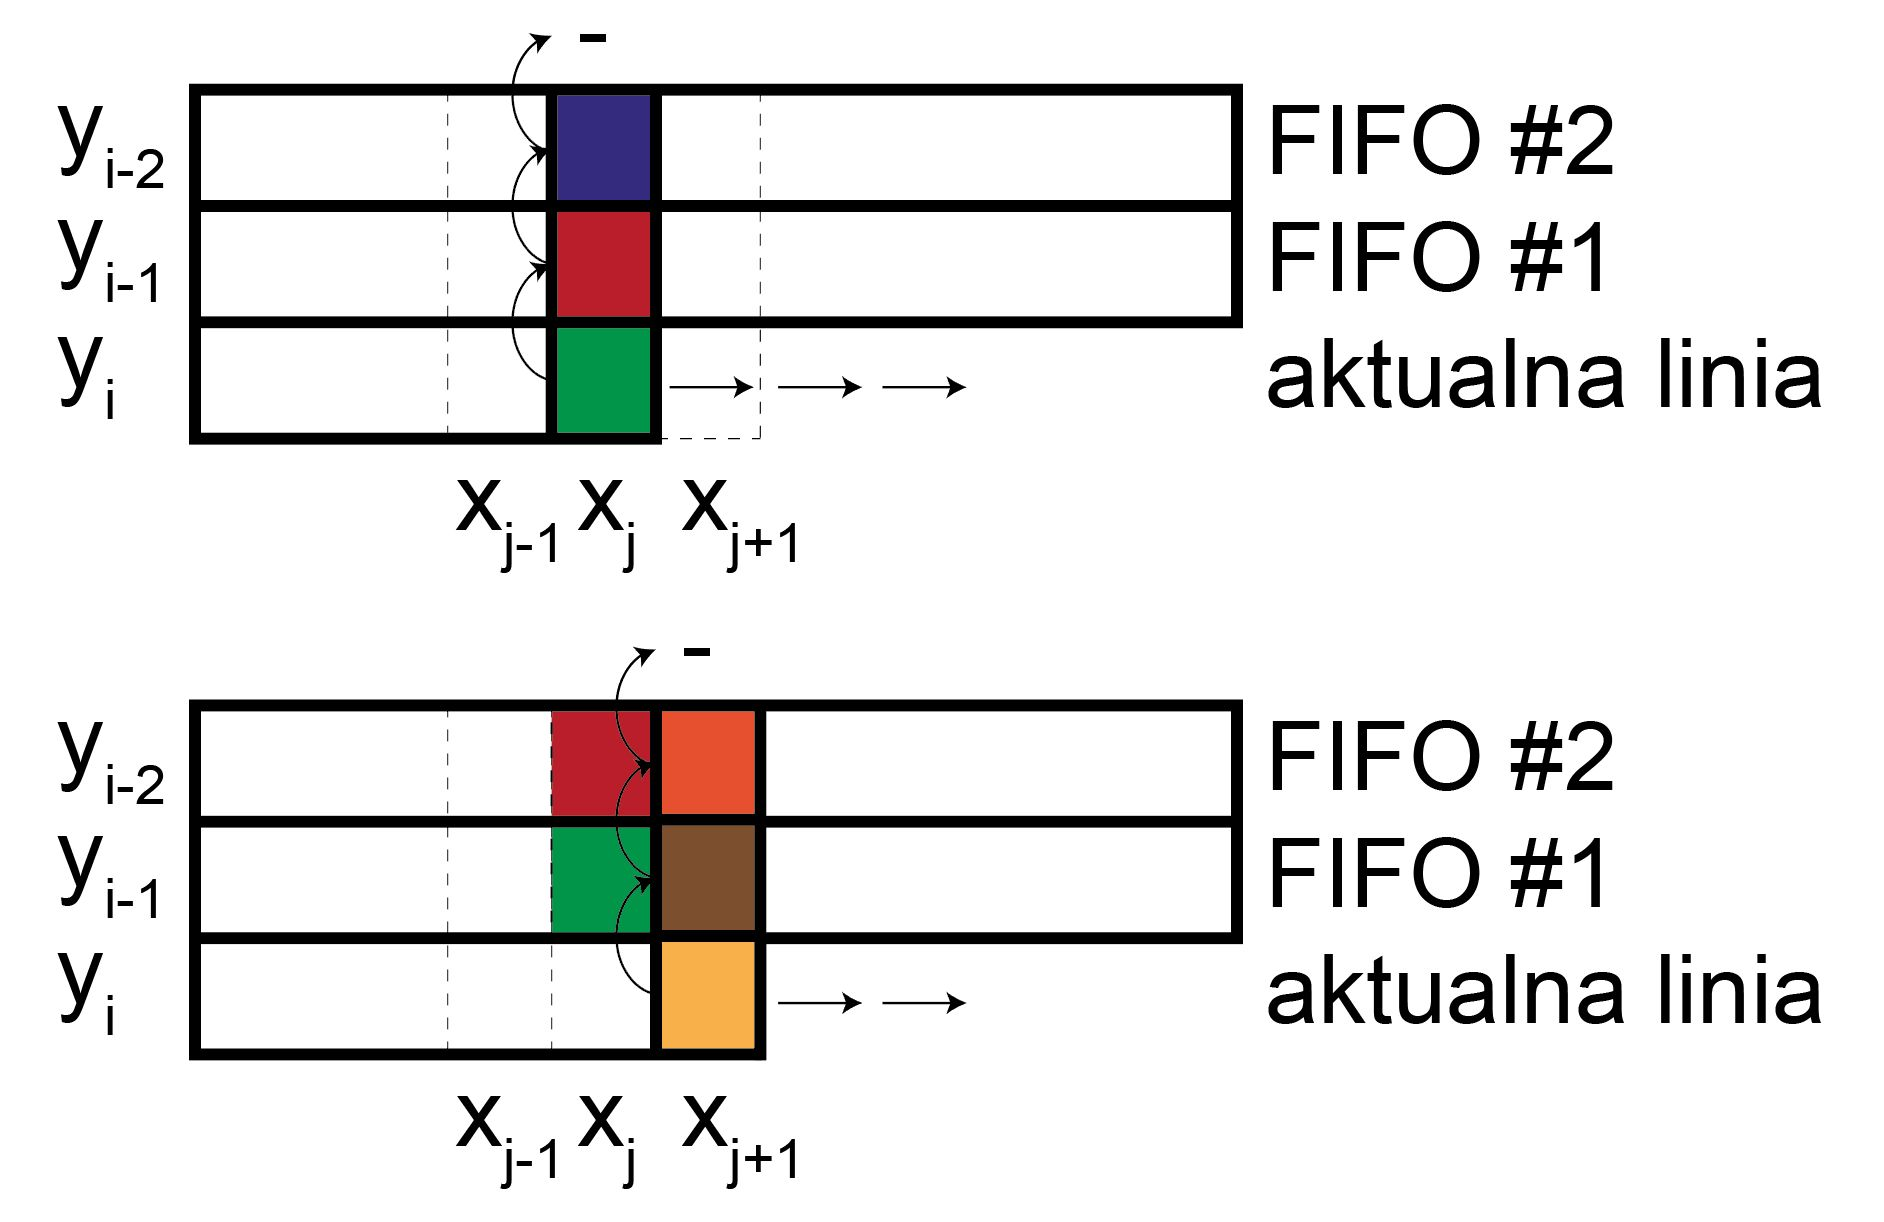
\includegraphics[width=11cm]{4_fifo_gradient.jpg}
	\caption{Schemat działania kolejek FIFO w procesie obliczania gradientu pionowego}
	\label{fig:fifo_gradient}
\end{figure}

Obliczanie gradientu poziomego nie nastręcza już tak wielu trudności - sąsiadujące ze sobą piksele pojawiają się tuż po sobie, jednak w tym wypadku zamiast aktualnych wykorzystywane są piksele wychodzące z FIFO \#1 i zapamiętywane w rejestrze przesuwnym. Oznacza to, że w chwili pojawienia się na wejściu do modułu nowego piksela ($i,j$), obliczony zostanie gradient poziomy piksela ($i-1,j-1$). Przez tę latencję potrzebne jest również nieznaczne opóźnienie gradientu pionowego, by obie wartości były zsynchronizowane i ustawione na wyjściu w tym samym momencie.

Sytuacje opisane powyżej dotyczą gradientów dla pikseli wewnątrz obrazu. Dla piksela znajdującego się na „początku” obrazu (lewa oraz górna krawędź), gradientem będzie dwukrotność różnicy pomiędzy nim a jedynym jego sąsiadem - w odpowiedniej osi. 

Piksele znajdujące się przy prawej i dolnej krawędzi ekranu wymagają innego podejścia. Poprzednie obliczenia były przeprowadzane w oparciu o sygnał aktywnego piksela ($valid$), którego zbocza były wykorzystywane do obliczeń gradientów aż do przedostatniego wiersza i kolumny obrazu ($i-1, j-1$). W tym przypadku, ich brak wymagał stworzenia logiki kontynuującej obliczenia i generującej wyjściowe sygnały aktywne. Brak dotychczasowych sygnałów \textit{valid} to również brak nowych danych dla kolejek FIFO, co skutkuje ich spodziewanym opróżnieniem krótko po odebraniu pełnej ramki obrazu. O ile poprzednio tempo obliczania gradientu było podyktowane pojawianiem się nowych pikseli i bezpośrednio powiązane z zastosowaną skalą, to w tym przypadku logika korzysta wyłącznie z opróżnianych kolejek FIFO, redukując odstęp pomiędzy wynikami do minimum (1 cykl zegara), co jest w zasadzie bez znaczenia dla dalszych obliczeń.

\subsection{Histogram gradientów}

Etapem następującym po uzyskaniu gradientu jest obliczenie wartości $arctg(\frac{g_y}{g_x})$. Wykorzystano tutaj blok IP CORDIC, który na wejściu spodziewa się wektora złożonego z licznika oraz mianownika o tych samych długościach, przy czym jego całkowita długość jest zaokrąglana do wielokrotności liczby 16. Gradienty uzyskane z poprzedniego modułu są zapisane w notacji S9.1, zatem wektor wejściowy musi mieć długość 32 - po 16 bitów na oba gradienty. Bardziej znaczące bity tych połówek zostały wypełnione zerami i nie mają znaczenia dla obliczeń. \newline 
Moduł będzie rozpoczynać obliczenia dla danych wejściowych tylko w przypadku, gdy policzone zostały oba gradienty (dwa niezależne sygnały \textit{valid\char`_x/y}), oraz gdy przynajmniej jeden z nich jest różny od zera ($\frac{0}{0}$ jest elementem nieoznaczonym, z którego nie sposób policzyć implementowaną funkcję). Opisane warunki \textit{valid\char`_x/y}, spięte odpowiednimi operatorami logicznymi, podłączono jako sygnał aktywny modułu. 

Otrzymane wartości należy następnie umieścić w dziewięciu 20-stopniowych przedziałach, co opisuje schemat \ref{fig:hog_gradient}. 
\begin{figure}[!ht]
	\centering
	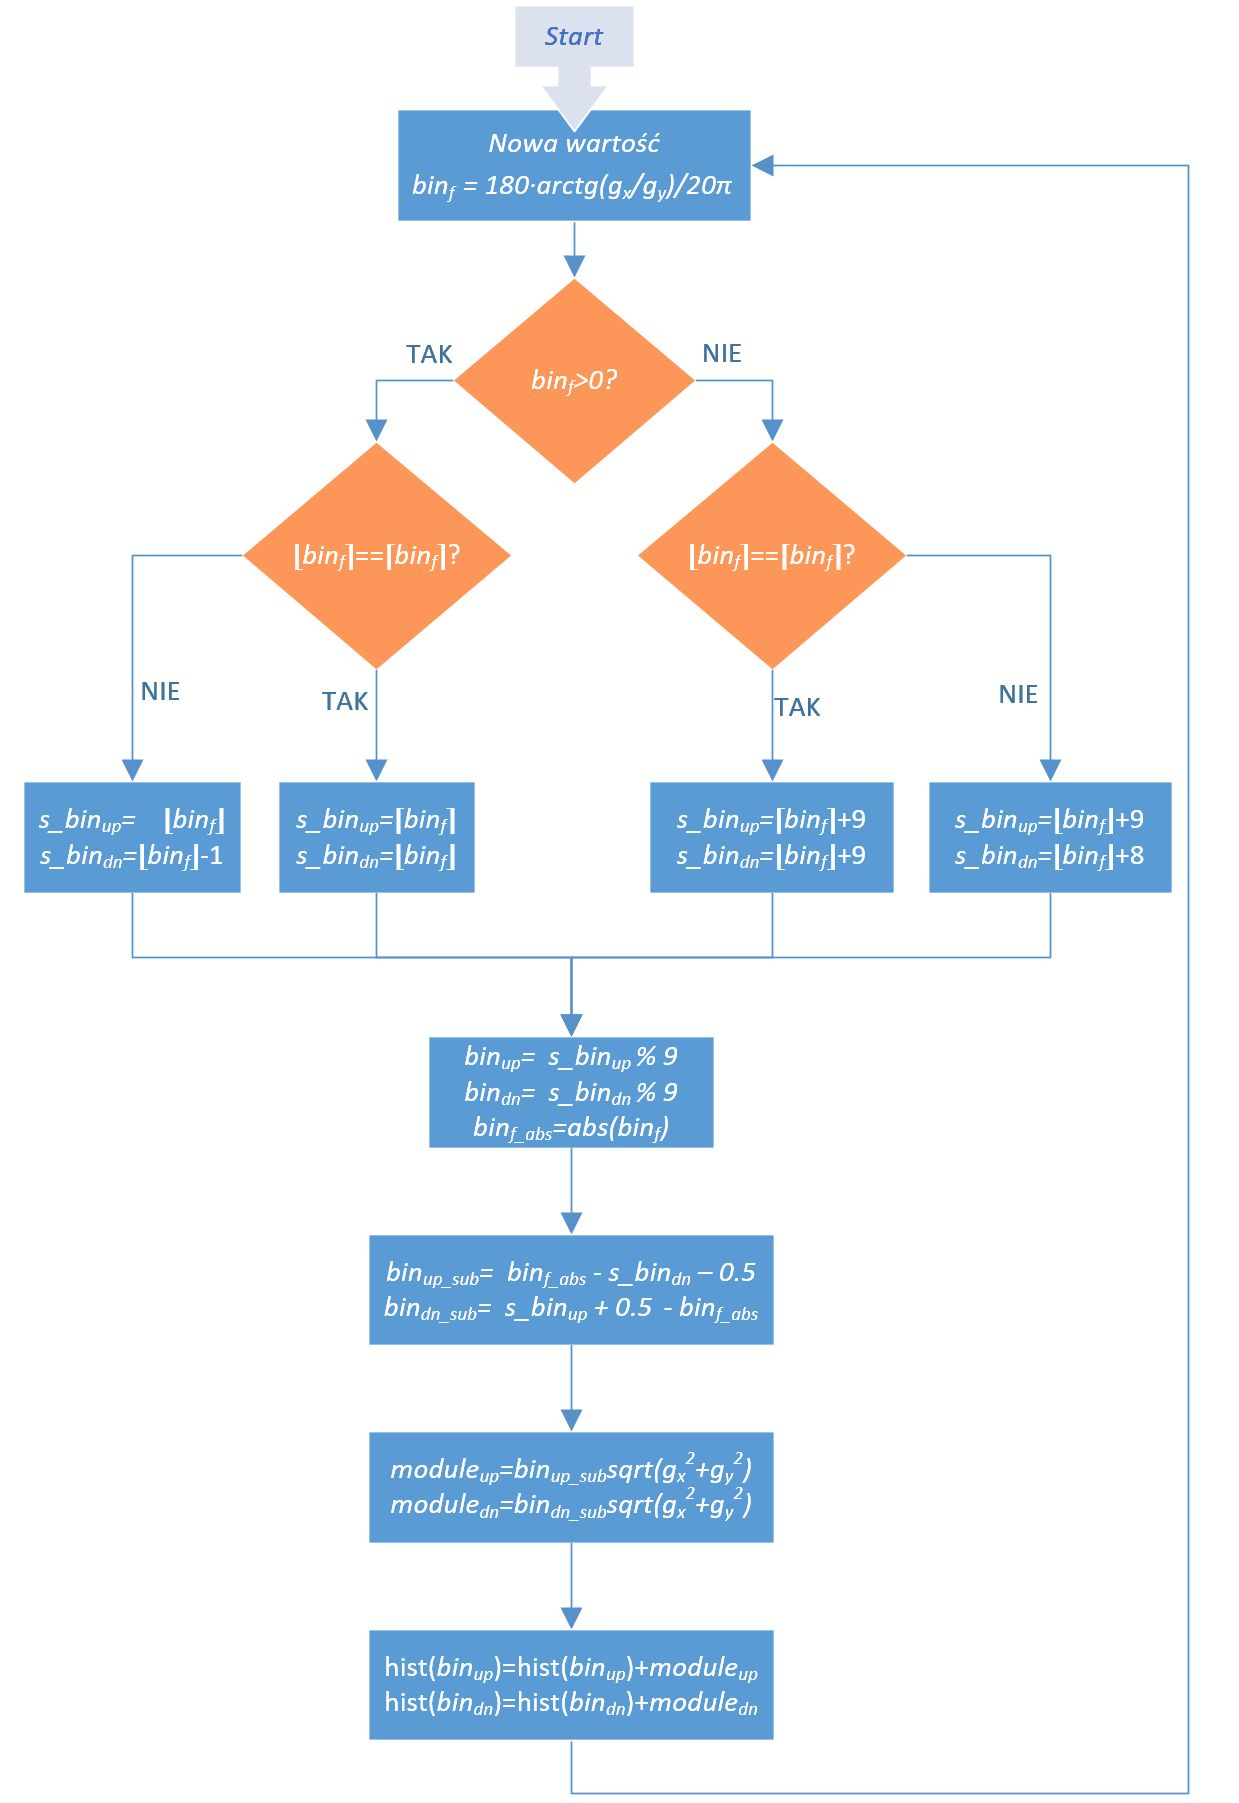
\includegraphics[width=12cm]{4_HOG_gradients.jpg}
	\caption{Schemat działania obliczeń prowadzących do utworzenia histogramu gradientów}
	\label{fig:hog_gradient}
\end{figure}
Pierwszym krokiem jest operacja mnożenia kątów podanych w radianach przez $\frac{180}{20\pi}$, która konwertuje je do liczb ułamkowych stanowiących wstępny przydział (niech będzie to $bin_f$).

Następnie, w zależności od położenia względem środka danego przedziału, wybierane są przedziały: górny i dolny w postaci liczb całkowitych: $s\_bin_{up}$ oraz $s\_bin_{dn}$. Ostateczne przedziały będą wymagać jednak normalizacji do postaci liczb z zakresu 0-8. Na ich podstawie tych wartości histogram powiększy dwa przedziały o interpolowane wartości modułu gradientów. 

Podstawową informacją wykorzystywaną w dalszej interpolacji jest odległość $abs(bin_f)$ od środków przedziałów $s\_bin_{up}$ oraz $s\_bin_{dn}$. Na tej podstawie obliczane są $module_{up}$ oraz $module_{dn}$ których suma jest równa modułowi gradientów.

Sam fragment logiki odpowiedzialny za obliczenie modułu został zrealizowany przy użyciu dwóch mnożarek dla obu gradientów, a sumę ich kwadratów następnie poddano pierwiastkowaniu blokiem CORDIC. Suma mnożeń jest wektorem U21.2, który poprzez dopisanie bitu '0' rozszerzono do U21.3. Zgodnie z dokumentacją modułu, wektor o tej długości jest traktowany przez CORDIC IP jako U1.23 - zatem jest wirtualnie przemnożony przez $2^{20}$. Wartość wyjściową należy później interpretować jako U11.13 (wirtualnie podzieloną przez $\sqrt{2^{20}}=2^{10}$). \newline
Ostateczne informacje - to jest dane o przedziałach i odpowiadające im części modułu zostały przekazane dalej, wraz z wygenerowanymi sygnałami aktywnymi.

Cały powyższy fragment podrozdziału skupiał się na operacjach związanych z pojedynczym pikselem. Teraz należy spojrzeć jednak z innej perspektywy, mianowicie na grupowanie pikseli w komórki, bloki i tworzenie wektorów cech na podstawie histogramu. \newline
Jak opisano we wstępie do rozdziału, najlepszy rezultat detekcji osiągnie się, realizując klasyfikację jak największej ilości wektorów cech wygenerowanych na obszarach z względnie niewielkim przesunięciem - jak zilustrowano to na \ref{fig:HOG_mesh}. Szybki przyrost zużycia zasobów układu ogranicza implementację do przetwarzania określonej ilości obszarów w sąsiedztwie miejsca podejrzewanego o obecność postaci.
Dane są bowiem zapisywane w pamięci BRAM. By nie marnować cennego miejsca w blokach BRAM, zdecydowano się zapisywać surowe histogramy, a nie gotowe wektory cech - wiedząc, że dalsza logika dokonując odczytu z tej pamięci, w odpowiedni sposób przekaże te informacje do klasyfikatora. Ostatecznie, pojedyncze okno detekcji $128\times 64$ to $32\cdot16=512$ histogramów, czyli $4608$ wartości. Wektor cech to aż $31\cdot15\cdot4\cdot9=16740$ wartości. Oszczędność wynikająca z zapisu pojedynczych histogramów pozwoli utworzyć znacznie więcej wektorów cech. Przykładowo, dla okna o wielkości $144\times 96$ należy zapisać $7776$ wartości. Pozwala to jednak wygenerować $9\cdot5=45$ wektorów cech - gdyby zaś wpisywać je do pamięci w gotowej formie, wymagałoby to aż $16740\cdot45=753300$ pozycji.

Pamięć RAM należy potraktować jako zbiór 9-elementowych histogramów ułożonych obok siebie. Przetwarzanie obrazu, rozumianego jako obiekt dwuwymiarowy, wymaga odpowiedniego mapowania tworzonych wartości do postaci jednowymiarowej, adresowej. Schemat \ref{fig:hog_histogram_scheme} przedstawia sposób pracy na ramce obrazu w kontekście zapisu do pamięci. Symbolem „$<=$” określa się przypisanie nieblokujące, które rzeczywisty efekt będzie miało dopiero na następnym zboczu narastającym zegara.
 
\begin{figure}[!ht]
	\centering
	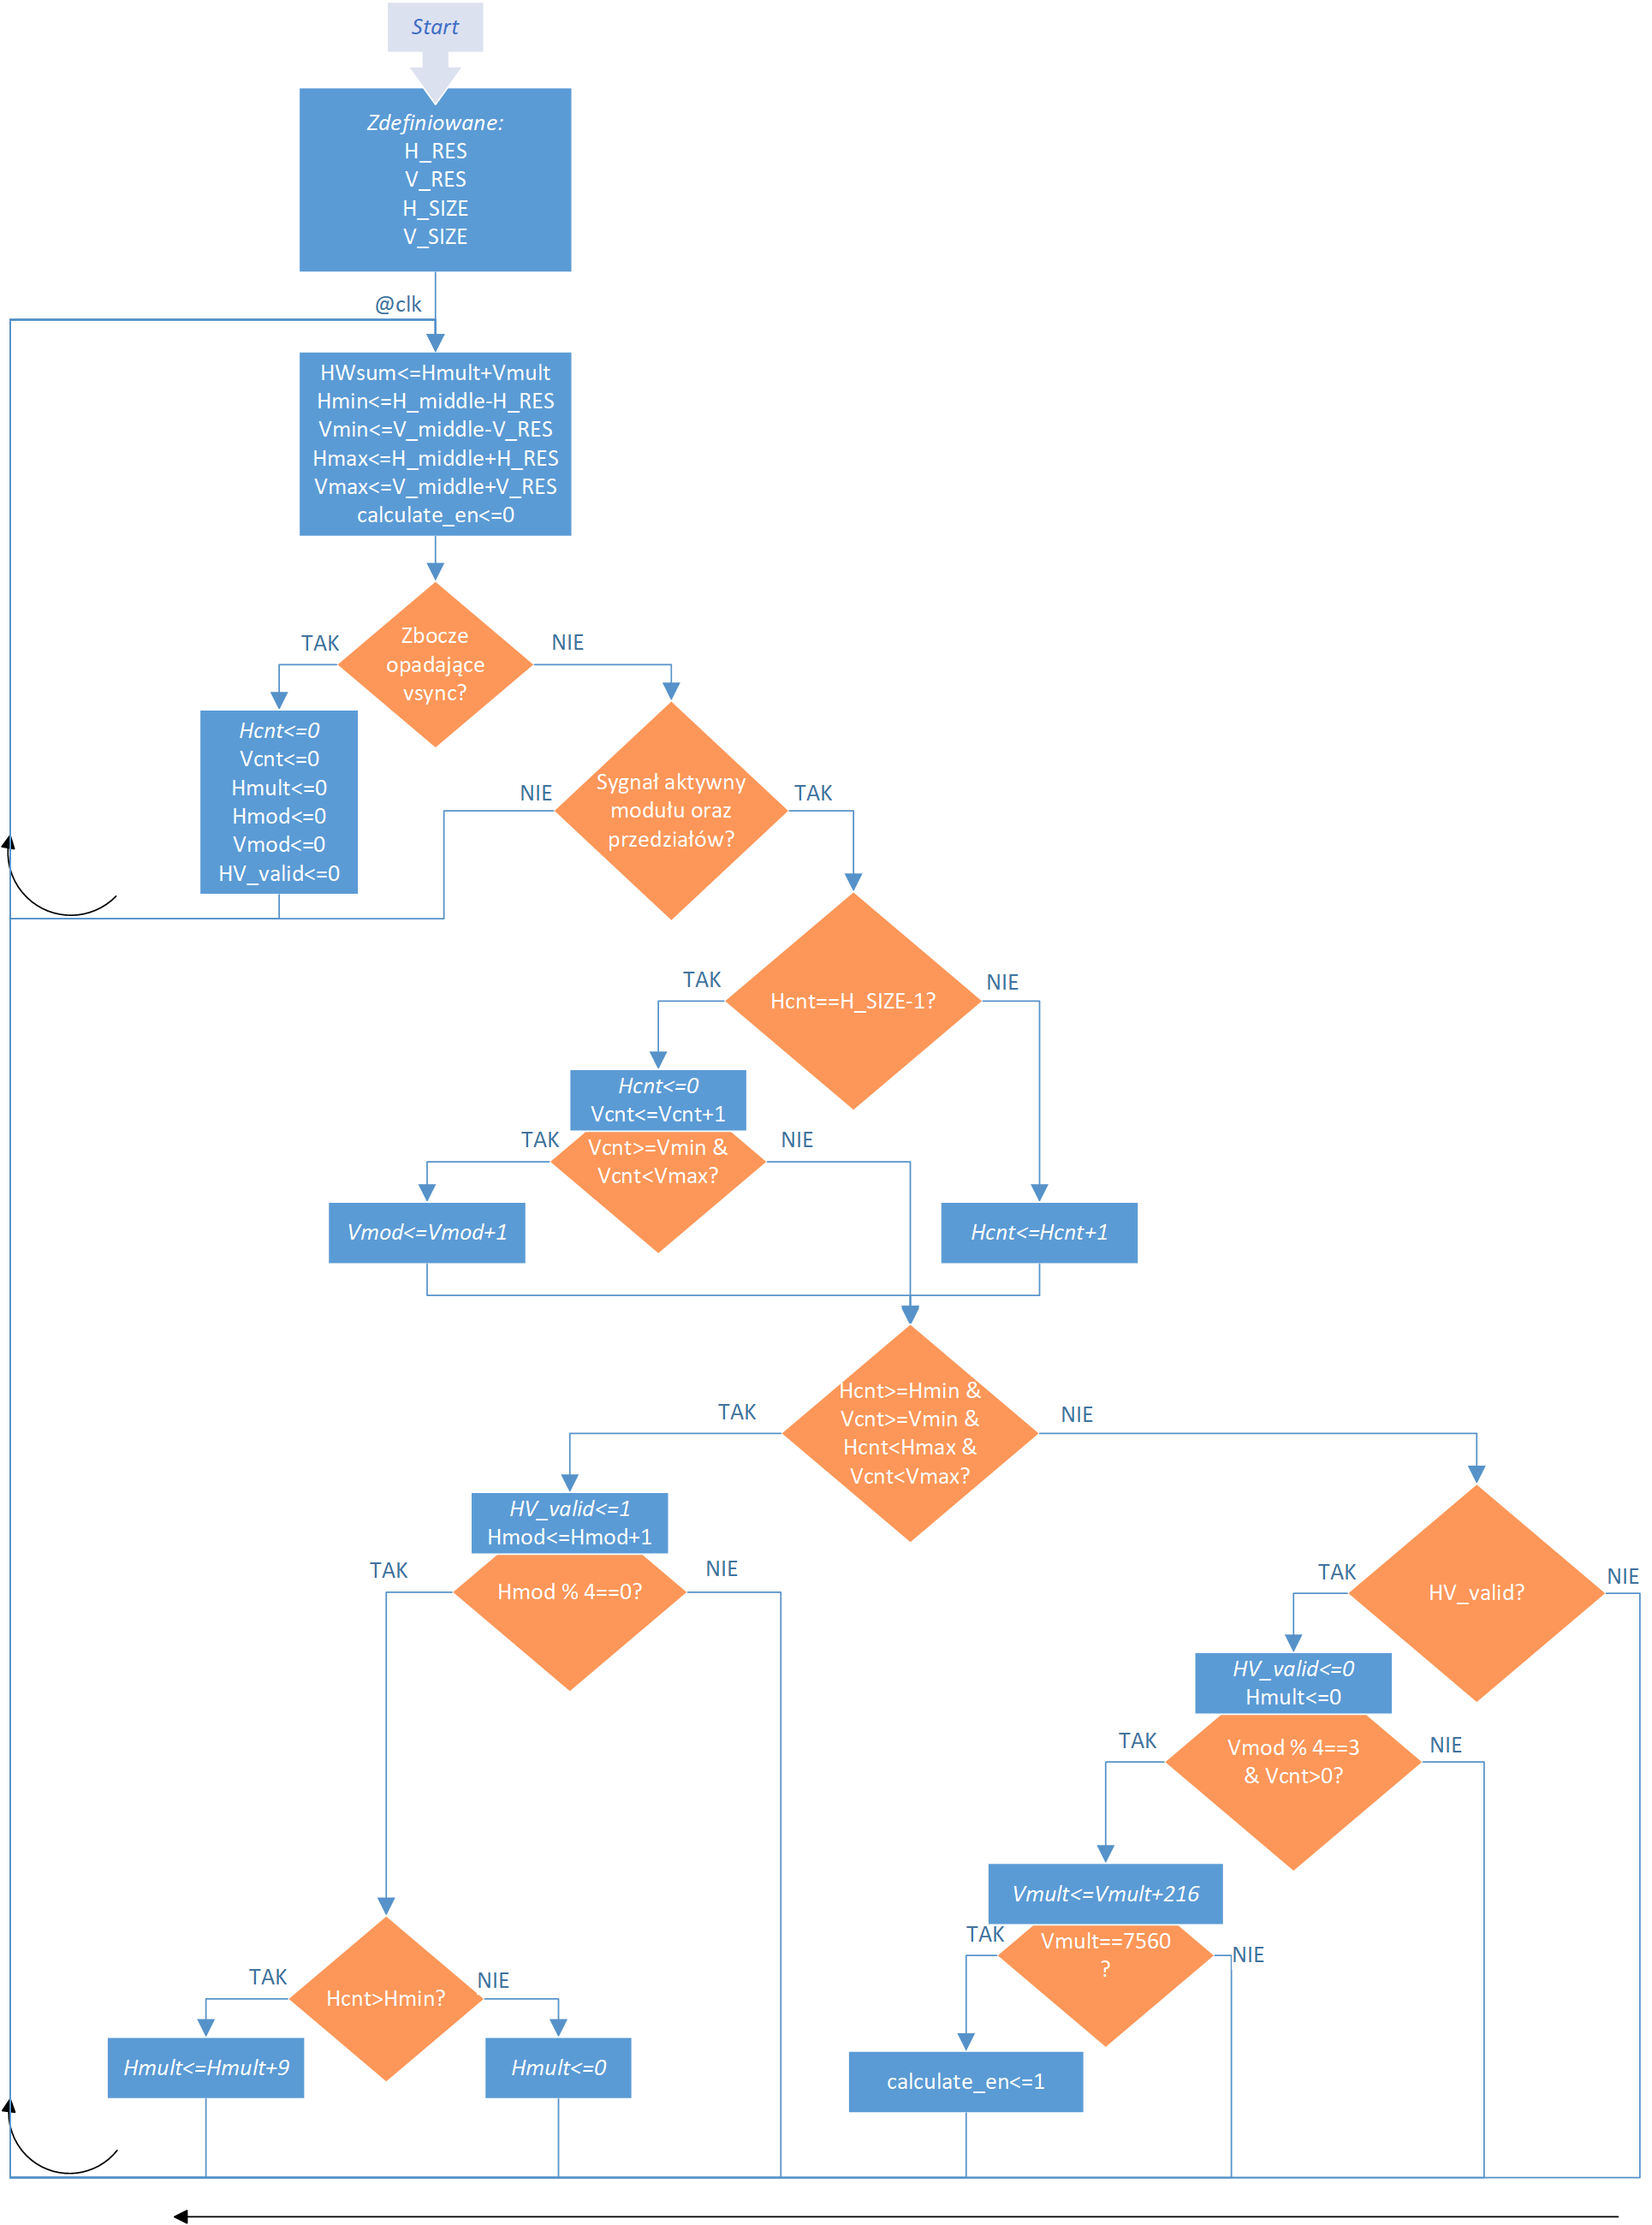
\includegraphics[width=16cm]{4_HOG_Histograms.png}
	\caption{Procedura wyboru adresu pamięci RAM w oparciu o pozycję aktualnego piksela}
	\label{fig:hog_histogram_scheme}
\end{figure} 
 
Określenie aktualnego położenia na obrazie jest możliwe dzięki zastosowaniu liczników, opierających swoje działanie na obecności sygnału aktywnego. Wykorzystano następujące parametry:
\begin{itemize}
	\item \textit{H\_SIZE}, \textit{V\_SIZE} - rozdzielczość obrazu przeskalowanego (indywidualnie dla każdej skali),
	\item \textit{H\_middle}, \textit{V\_middle} - koordynaty piksela środkowego, będącego w centrum analizowanego obszaru (w odniesieniu do odpowiedniej skali, dostarczone przed rozpoczęciem analizy pełnej klatki),
	\item \textit{H\_RES}, \textit{V\_RES} - wartości określające zasięg analizowanego obszaru - w odległości od piksela środkowego,
\end{itemize}
oraz zmienne:
\begin{itemize}
	\item \textit{Hcnt}, \textit{Vcnt} - zmienne inkrementowane odpowiednio do wartości maksymalnych \textit{H\_SIZE}, \textit{V\_SIZE} - pozwalają określić aktualne położenie na obrazie (i względem analizowanego obszaru),
	\item \textit{HV\_valid} - sygnał aktywny informujący o aktualnym położeniu wewnątrz analizowanego obszaru,
	\item \textit{Hmod}, \textit{Vmod} - liczniki modulo służące do rozdzielenia pikseli wchodzących w skład różnych histogramów (kwadratów o boku $4\times 4$),
	\item \textit{Hmult}, \textit{Vmult} - zmienne będące bazą adresową do zapisu aktualnego histogramu (horyzontalna zmienna powiększana o $9$, wertykalna o $9\cdot24$ - ilość histogramów w linii poziomej),
	\item \textit{calculate\_en} - sygnalizacja zakończonego procesu obliczania i zapisywania histogramów - możliwość rozpoczęcia klasyfikacji dla danej skali,.
\end{itemize}

Pamięć histogramu pracuje w trybie True Dual Port, umożliwiając jednoczesny dostęp do dwóch interpolowanych przedziałów aktualnego histogramu, $s\_bin_{up}$ oraz $s\_bin_{dn}$. Ich adresy są przedstawione równaniem:
\begin{equation}
\label{eq:adressing_hist}
\left.\begin{aligned} 
addr_{up}&=Hmult+Vmult+s\_bin_{up} \\ 
addr_{dn}&=Hmult+Vmult+s\_bin_{dn}
\end{aligned}\right.
\end{equation}
Zapis danych do pamięci histogramu jest realizowany, uprzednio odczytując aktualne wartości komórek i powiększając je odpowiednio o części modułu: $module_{up}$ oraz $module_{dn}$.



\subsection{Uczenie}
Uczenie to żmudny proces przetworzenia obrazów i ekstrakcji wektorów cech, na podstawie których powstanie płaszczyzna rozdzielająca próbki pozytywne od negatywnych. Przejście przez tak wielką ilość obrazów ma charakter jednorazowy, po którym będzie dysponować się parametrami umożliwiającymi klasyfikację. Z tego względu nie zdecydowano się na implementację modułu uczącego w układzie FPGA - tak ze względu na złożoność tego etapu, czas trwania procedury, jak i prawdopodobnie duży udział modułu w zużyciu zasobów logiki. 

Wybór padł na środowisko MATLAB, w którym zresztą wcześniej stworzono prototyp całego algorytmu (model programowy). Skrypt korzysta z plików tekstowych zawierających listy próbek do wczytania, które ostatecznie muszą być w rozmiarze $128\times 64$. Jak widać na ilustracji \ref{fig:HOG_image_examples}, wymiary próbek negatywnych mocno odbiegają od założonego wymiaru klasyfikowanego obrazu ($128\times 64$). Zdecydowano, iż w ich przypadku uczeniu poddany będzie obszar o wymiarach 128x64 wycięty ze środka oryginałów, jak i obraz przeskalowany oraz obcięty do wymiarów $128\times 64$. Na bazie tak przygotowanych próbek powstaje tablica deskryptorów oraz druga, która przechowuje odpowiadające im wartości klas (1 lub 0). Z obu tablic korzysta wbudowana funkcja \textit{svmtrain}, która zwraca strukturę ze współczynnikami. Z kolei \textit{svmclassify} jest w stanie odpowiednio zaklasyfikować obraz (a właściwie jego deskryptor). Tę funkcję użyto w procesie testowania niezależnego zestawu danych, by sprawdzić skuteczność wygenerowanych parametrów. Etap testowania jest dodatkowo przydatny - pozwala na bazie eksperymentów zdefiniować optymalny rozmiar komórki (kwadratu pikseli), na bazie których liczony jest pojedynczy histogram. Tabela \ref{tab:HOG_cell_size} prezentuje wyniki. Ekperyment przeprowadzono na komputerze wyposażonym w procesor Intela klasy i7, trzeciej generacji.
\newcolumntype{P}[1]{>{\centering\arraybackslash}p{#1}}
\begin{table}[h]
	\centering
	\captionsetup{justification=centering,margin=1cm}
	
	\begin{tabular}{|P{3cm} |P{3cm} |P{4.5cm}| P{3.5cm}|}	
		\hline
		\rowcolor{lightgray} Rozmiar komórki [px] & Ilość elementów wektora cech & Błąd klasyfikacji [\%]  & Czas trwania algorytmu [s] \\ 
		\lbrack$2\times $2\rbrack			& 70308		& 3.4069		& 52min 42s		\\ 
		\hline		
		\lbrack$4\times 4$\rbrack			& 16740 	& 2.3344		& 14min 08s		\\ 
		\hline
		\lbrack$8\times 8$\rbrack			& 3780		& 3.3438		& 05min 01s		\\ 
		\hline
		\lbrack$16\times 16$\rbrack			& 756		& 5.1735		& 02min 50s		\\ 
		\hline
	\end{tabular}
	
	\caption{Skuteczność algorytmu na zbiorze testowym w zależności od wielkości pojedynczej komórki}
	\label{tab:HOG_cell_size}
\end{table}
\newline
Okazuje się, że algorytm wykazuje największą skuteczność dla komórki o rozmiarze $4\times 4$ - zdecydowano się zatem na implementację algorytmu HOG w układzie FPGA właśnie w oparciu o tę wartość parametru. Szybkie obliczenia pokazują, że dla obrazu o wymiarach $128\times 64$ powstanie $32\times 16$ komórek, a idąc dalej, $31\times 15$ bloków po 4 histogramy po 9 wartości, czyli długość wektora cech będzie wynosić 16740. Oznacza to również, że po zakończonym procesie uczenia powstanie wektor współczynników o takiej długości.

Założeniem jest, by podczas pracy systemu wbudowanego nie ingerować we współczynniki, a raczej opierać się na pierwotnych wynikach uczenia. Dane te muszą być przechowane w odpowiedni sposób, by możliwy był do nich prosty i szybki dostęp. Postanowiono zapisać wektor w pamięci ROM inicjalizowanej plikami \textit{*.mem}, utworzonymi podczas wykonywania skryptu uczenia w MATLABie. Ręcznie dostosowany moduł pamięci posiada trzy niezależne sektory (w zakresie adresowania i długości danych), inicjalizowane następującymi informacjami: 

\begin{itemize}
	\item składniki skalujące - 16740 elementów wymaganych do przesunięcia każdego elementu wektora cech. Wartości w przedziale: $<-0.2616, -0.0527>$; precyzja zapisu: S0.11.
	\item czynniki skalujące - 16740 elementów do przemnożenia z powyższymi sumami. Wartości w przedziale: $<4.4207, 12.6310>$; precyzja zapisu: U4.8.
	\item współczynniki maszyny wektorów nośnych. Wartości w przedziale: $<   -0.0076, 0.0063>$; precyzja zapisu: S0.15 (oryginalnie w formacie S0.22, lecz 7 najstarszych bitów ma zawsze postać bitu znaku).
\end{itemize}

Dodatkowym współczynnikiem jest wartość przesunięcia gotowego wyniku o precyzji S0.40, jednak jest ona przechowywana w logice. 
Powyższa pamięć zajmuje aż 40 z wszystkich 140 bloków BRAM. Należy zauważyć, iż wymusza to współdzielenie pojedynczej instancji modułu we wszystkich procesach klasyfikacji. Z tego względu istotne jest stworzenie logiki synchronizującej początek przetwarzania wektorów cech ze wszytkich skal - opisuje to kolejna podsekcja.

\subsection{Klasyfikacja}
Etap klasyfikacji następuje bezpośrednio po obliczeniu wektorów cech. Odczytywane wartości pamięci ROM muszą być współdzielone pomiędzy obliczeniami przeprowadzanymi dla każdej ze skal obrazu, jednak w każdym przypadku tempo generowania histogramów nie jest jednakowe - proces przebiegnie szybciej dla większych obrazów (tam analizowany fragment obrazu pojawi się na wejściu wcześniej). O gotowości histogramów z odpowiedniej skali informuje indywidualny dla niej sygnał \textit{calculate\_en}. Dopiero w momencie otrzymania wszystkich sygnałów \textit{calculate\_en} (stan wysoki na wyjściu iloczynu logicznego) rozpoczynany jest właściwy proces klasyfikacji.

Moduł odpowiadający za sklasyfikowanie informacji pochodzących z pojedynczej skali zrealizowano w formie krótkiej maszyny stanu, na którą składają się następujące etapy:
\begin{itemize}
	\item inicjalizacja - oczekiwanie na sygnał \textit{full\_frame}, informujący o rozpoczęciu algorytmu na pełnej klatce obrazu
	\item czyszczenie pamięci przechowującej wektory cech z poprzednich uruchomień algorytmu - etap ten ma miejsce tuż po otrzymaniu sygnału \textit{full\_frame}, który pojawia się podczas stanu wysokiego synchronizacji pionowej; jest wykonywany na tyle szybko, by zdążyć przed pikselami wchodzącymi do modułu liczącego histogram.
	\item oczekiwanie na iloczyn sygnałów \textit{calculate\_en}; inicjalizacja zmiennych algorytmu
	\item właściwa klasyfikacja
\end{itemize}

O ile zapisane w pamięci ROM współczynniki mają postać wektora cech, tak pamięć RAM przechowuje nieuporządkowane fragmenty histogramów. Wymagało to stworzenia logiki, która skleja ze sobą dane z odpowiednich adresów pamięci, interpretując je w postać deskryptora. Opisuje to poniższy diagram.

\begin{figure}[!ht]
	\centering
	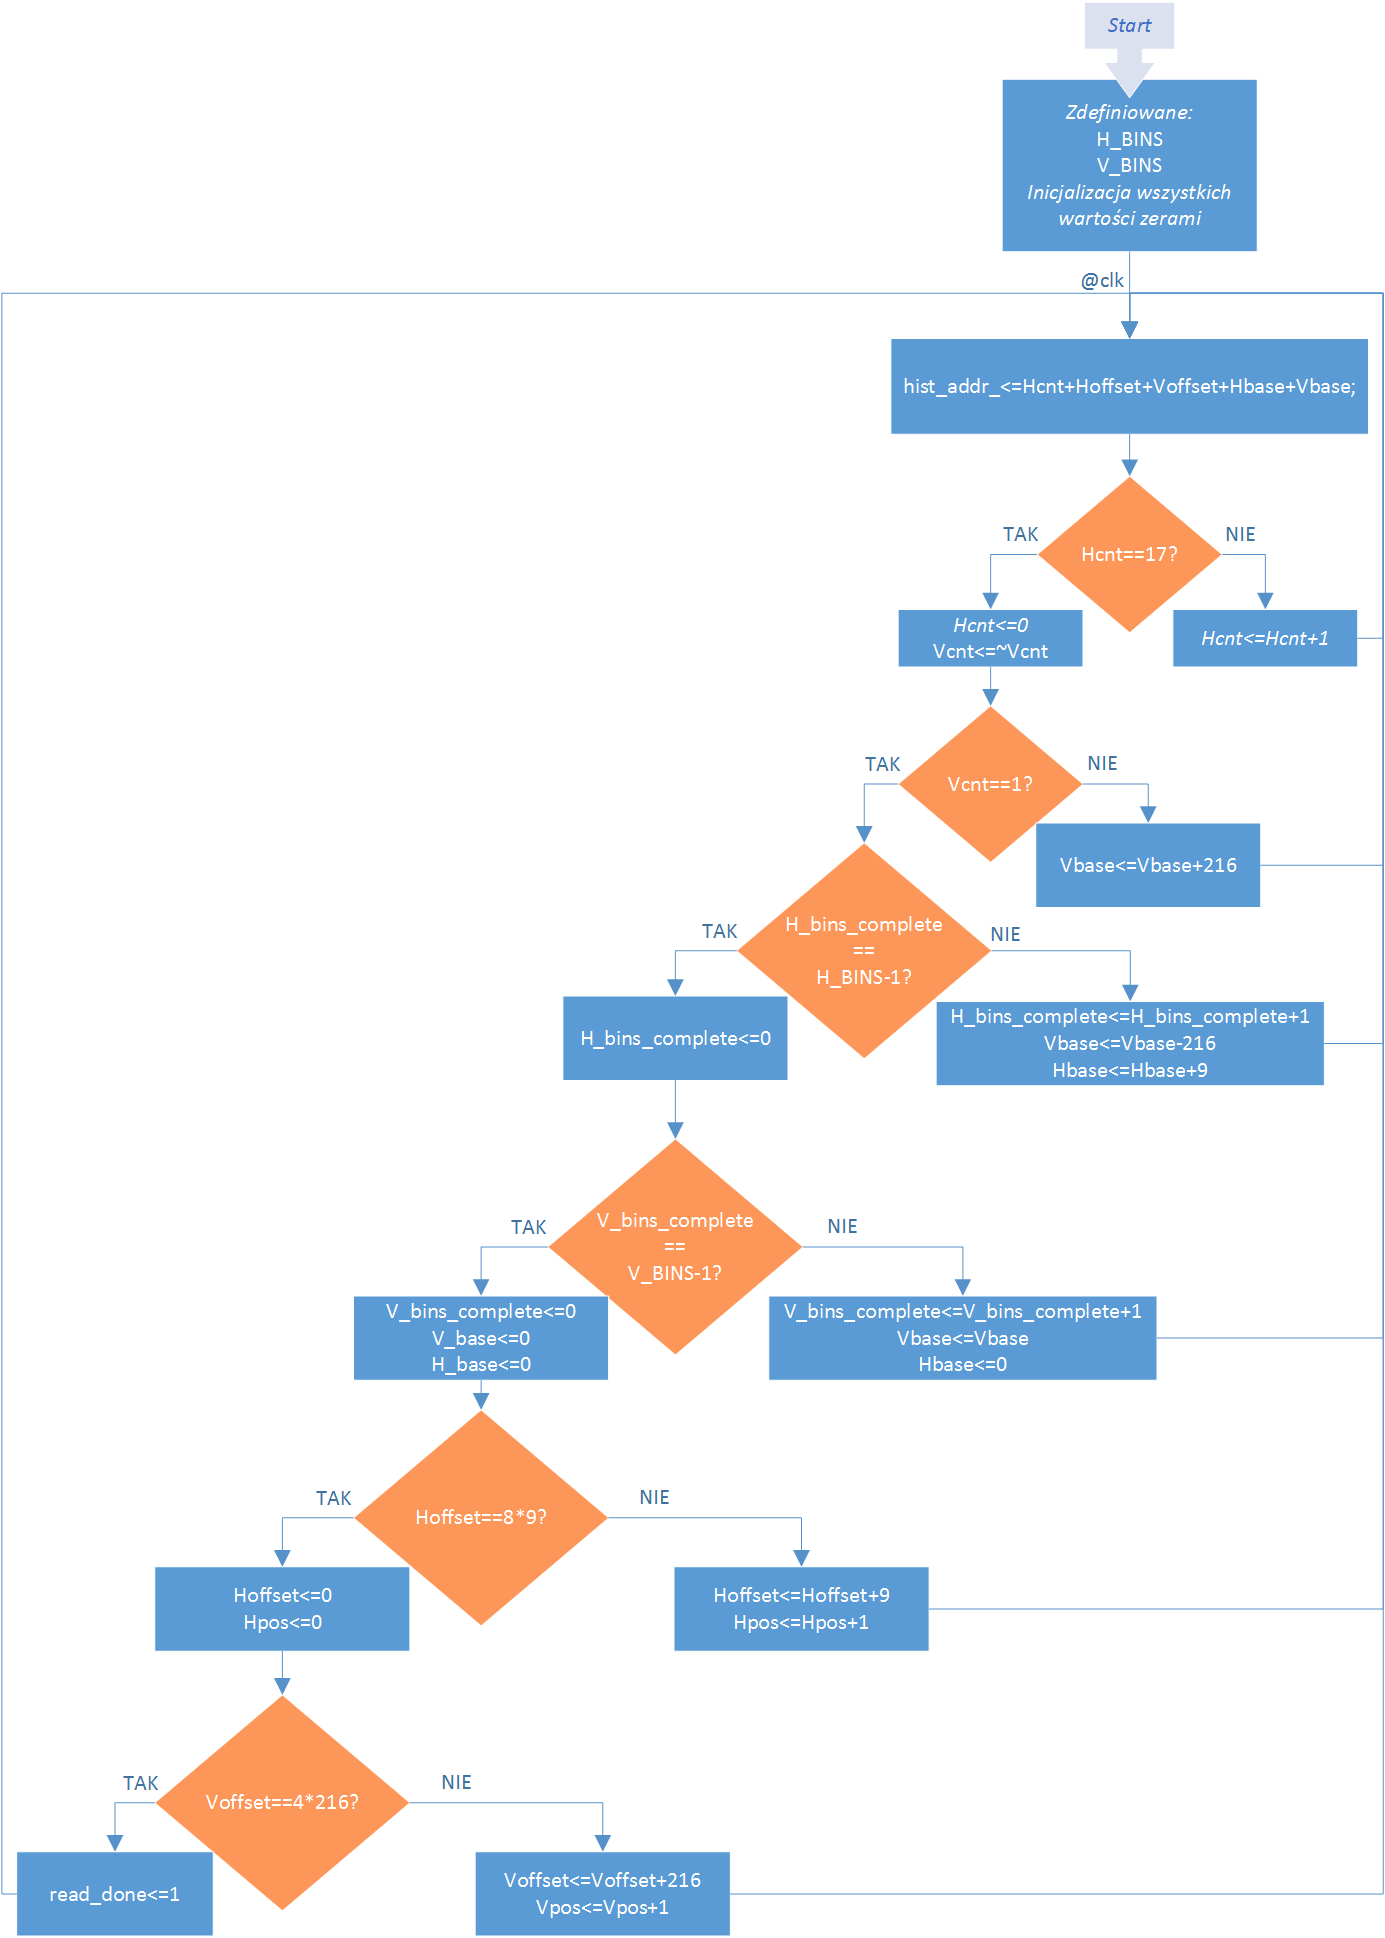
\includegraphics[width=16cm]{4_HOG_Features.png}
	\caption{Procedura wyboru adresu pamięci RAM w procesie odczytu kolejnych histogramów}
	\label{fig:hog_feature_histrogram_address}
\end{figure} 

Kolejnym etapem jest normalizacja bloków, która ze względu na prostszą realizację została umieszczona wewnątrz procesu klasyfikacji (chociaż właściwie idea bloków nie funkcjonowała we wcześniejszych modułach). Blokiem jest struktura 4 histogramów, czyli łącznie 36 wartości. Odczytane z pamięci RAM dane są podnoszone do kwadratu przez mnożarkę, a następnie inkrementowane. Suma 36 takich wartości jest pierwiastkowana i będzie stanowić mianownik w procesie normalizacji powiązanego bloku (zgodnie z równaniem \ref{eq:HOG_norm3}). Moduł pierwiastkujący działa potokowo, więc zwraca również wartość pierwiastkową z niepełnych sum - dlatego ważne jest wygenerowanie sygnału aktywnego w momencie zsumowania 36 elementów, a także zatrzaśnięcie poprawnej wartości pierwiastka na czas 36 dzieleń.

Normalizacja wymusza ponowne przejście przez odpowiednie dane pamięci RAM. Zastosowanie dwuportowego modułu pozwala na uzyskanie dostępu do uprzednio przetworzonych danych na drugim kanale, podczas gdy pierwszy port kontynuuje zwracanie informacji potrzebnych do obliczenia współczynników normalizacji dla kolejnych bloków. Poprawną kolejność danych na drugim porcie osiągnięto przez odpowiednie opóźnienie sygnału adresowego z portu pierwszego. 

Napływające potokowo dane z portu drugiego, podzielone przez odpowiedni współczynnik normalizacji, mają ustawioną flagę \textit{normalized\_valid}. Jej stan wysoki rozpoczyna  inkrementację adresu pamięci ROM przechowującej współczynniki przesunięć (\textit{shifts}). Każda z 16740 par zostanie do siebie dodana. Znormalizowane elementy wektora cech mają postać U11.13, zatem należało rozszerzyć wektor \textit{shifts}. 
\newline
Kolejnym krokiem jest wymnożenie każdej z sum przez czynnik skalujący, a następnie przez właściwy współczynnik maszyny wektorów nośnych. Aby to osiągnąć, należało ponownie i odpowiednio opóźnić linie adresowe uzyskujące dostęp do przestrzeni adresowej danych \textit{factors} oraz \textit{vectors}. Ostateczna szerokość pojedycznego elementu wynosi S0.40.

Docelowa wartość definiująca detekcję jest sumą wszystkich 16740 przetworzonych  elementów oraz jeszcze jednej stałej wyznaczonej na etapie uczenia, \textit{offset} równej $-0.6327$. \textit{Offset} stanowi wartość początkową sumy przy rozpoczęciu obliczeń nad kolejnym wektorem cech.
Ze względu na konieczność zapewnienia dobrej dokładności w procesie sumowania, wynik jest zapisywany w notacji S8.40, co wymaga rozszerzenia dodawanych elementów o 8 kopii najbardziej znaczącego bitu (będącego zresztą informacją o znaku).

\subsection{Przetwarzanie wyników}

Niezależnie od ilości przetwarzanych skal obrazu, całkowite zakończenie wszystkich klasyfikacji w systemie rozpocznie etap analizy wyników. Jest on dość prosty, gdyż zakłada jedynie porównanie najlepszych rezultatów ze wszystkich skal - w modułach klasyfikacji zaimplementowano logikę, która zapamiętuje swoje lokalne minima i parametry obszarów (w odpowiednich skalach), na podstawie których je osiągnięto. Skutkiem porównania jest wyłonienie skali z najlepszym wynikiem, a koordynaty tego obszaru zostają dostosowane do rozdzielczości natywnej i mogą być wykorzystane przez warstwę wyższą.



 
\chapter{Integracja układu FPGA z dronem}
Opisana w poprzednim rozdziale architektura sprzętowa dotyczyła dwóch algorytmów, które mogą funkcjonować niezależnie od siebie. Ostatecznie jednak istnieje jeszcze najwyższa warstwa logiczna, która pozwala wykorzystać je jak najlepiej, oraz odpowiada za komunikację z dronem.

\section{Konstrukcja drona}
Poniżej opisane są parametry wykorzystywanej maszyny:
\begin{itemize}
	 \item typ obiektu: hexacopter (rama DJI F550),
	 \item rodzaj śmigieł: wzmocnione śmigła o oznaczeniu 9050, czyli o średnicy śmigła równej $9.0"$ ($~22.86$cm) oraz skoku śmigła $5.0"$ ($~12.7$cm).,
	 \item silniki: DJI 2312/960KV sterowane kontrolerami 420 LITE
	 \item zasilanie: czterokomorowa bateria LiPo o nominalnym napięciu $14.8$V (maksymalnym $16.8$V) oraz o pojemności $6450$mAh,
	 \item kamera: Xiaomi Yi,
	 \item gimbal: Tarot T-2D,
	 \item aparatura radiowa: FrSky Taranis X9D Plus,
	 \item odbiornik: FrSky X8D,
	 \item autopilot: 3DR Pixhawk.
\end{itemize}
\subsection{Autopilot}

Każdy dron byłby bezużyteczną konstrukcją, gdyby nie serce maszyny - tzw. autopilot. W tym przypadku postanowiono wykorzystać urządzenie Pixhawk. Jest to zgodny ze standardami przemysłowymi moduł na otwartej licencji, stworzony przy współpracy z 3D Robotics oraz ArduPilot Group. Posiada następujące parametry:
\begin{itemize}
	\item procesor Cortex-M4F taktowany zegarem 168 MHz,
	\item sensory: trzyosiowy akcelerometr, żyroskop, kompas magnetyczny, barometr i zewnętrzny GPS,
	\item slot na kartę microSD,
	\item możliwość połączenia peryferiów (interfejsy: UART, I2C, CAN),
	\item 14 wyjść PWM (8 głównych z zabezpieczeniami + 6 dodatkowych).
\end{itemize}

\begin{figure}[h]
	\centering
	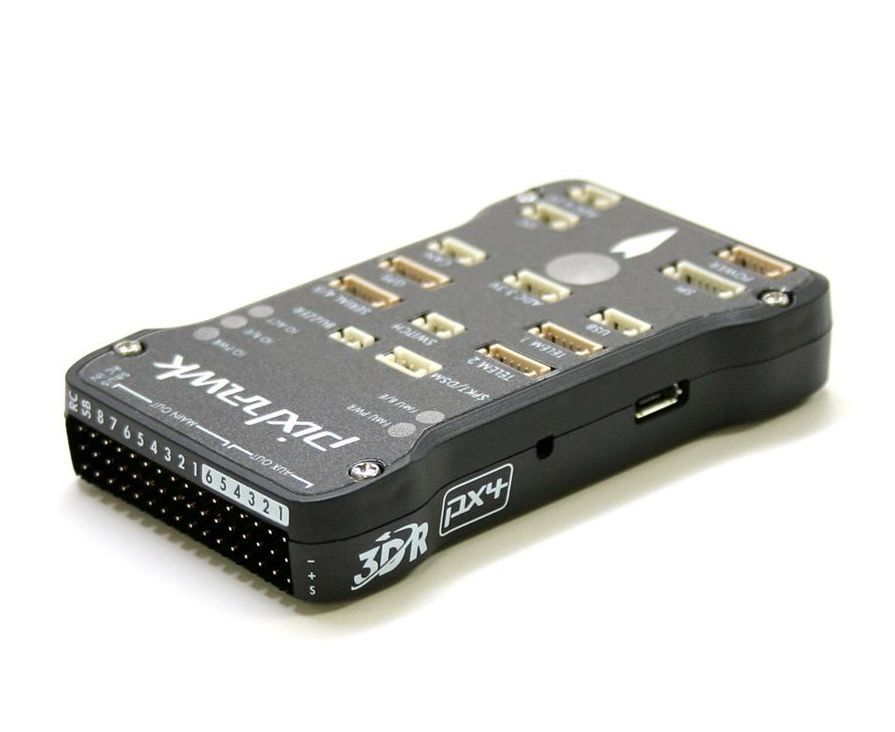
\includegraphics[width=8cm]{5_pixhawk.jpg}
	\caption{Autopilot Pixhawk - widok na panel główny oraz we/wy PWM}
	\label{fig:pixhawk}
\end{figure}

Powyższy sprzęt jednak nie jest w pełni skonfigurowany do pracy po wyjęciu z pudełka - szczególnie, że jako uniwersalny produkt, bywa montowany na konstrukcjach o szerokim rozrzucie parametrów. Może zapewnić sterowanie kopterom, samolotom modelarskim oraz nawet łazikom. W przypadku dwóch pierwszych grup konfiguracja wiąże się ze zdefiniowaniem odpowiedniej liczby śmigieł i ich rozstawienia, typu aparatury radiowej oraz zewnętrznych urządzeń geolokalizacyjnych. Tę dość dużą elastyczność mogą zapewnić dwa główne systemy, które są wczytywane z pamięci SD i pracują w czasie rzeczywistym. Dedykowany, PX4 Flight Stack jest stworzony przez twórców modułu, oraz ArduPilot Copter (ArduCopter) - niezależny, otwarty system, który został dostosowany do platformy Pixhawk z wykorzystaniem dostępnych narzędzi deweloperskich. Ze względu na większą bazę użytkowników i dojrzałość projektu, wybrano drugie rozwiązanie.

\begin{figure}[h]
	\centering
	\captionsetup{justification=centering,margin=1cm}
	\hspace*{0cm}
	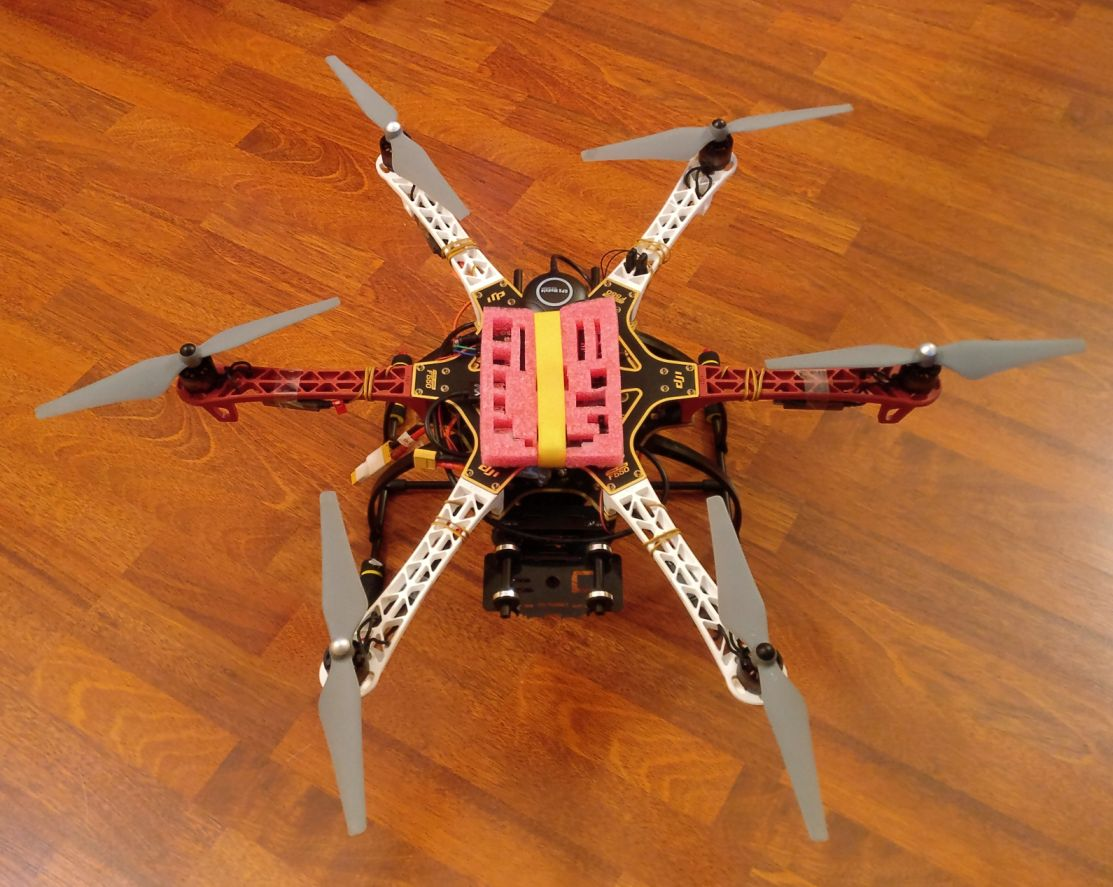
\includegraphics[width=14cm]{5_drone_photo.jpg}
	\caption{Zdjęcie przedstawiające w pełni wyposażonego drona. Pod gąbką ochronną skrywa się układ PYNQ}
	\label{fig:drone_photo}
\end{figure}

\subsection{Propagacja sygnałów}
Zbudowanie drona w oparciu o gotowe komponenty nie jest zadaniem skomplikowanym. Jednak w momencie, gdy doszły elementy zapewniające jego autonomizację, należało dokładnie przemyśleć jego przebudowę. Schemat \ref{fig:architecture} przedstawia architekturę sygnałową.
\begin{figure}[]
	\centering
	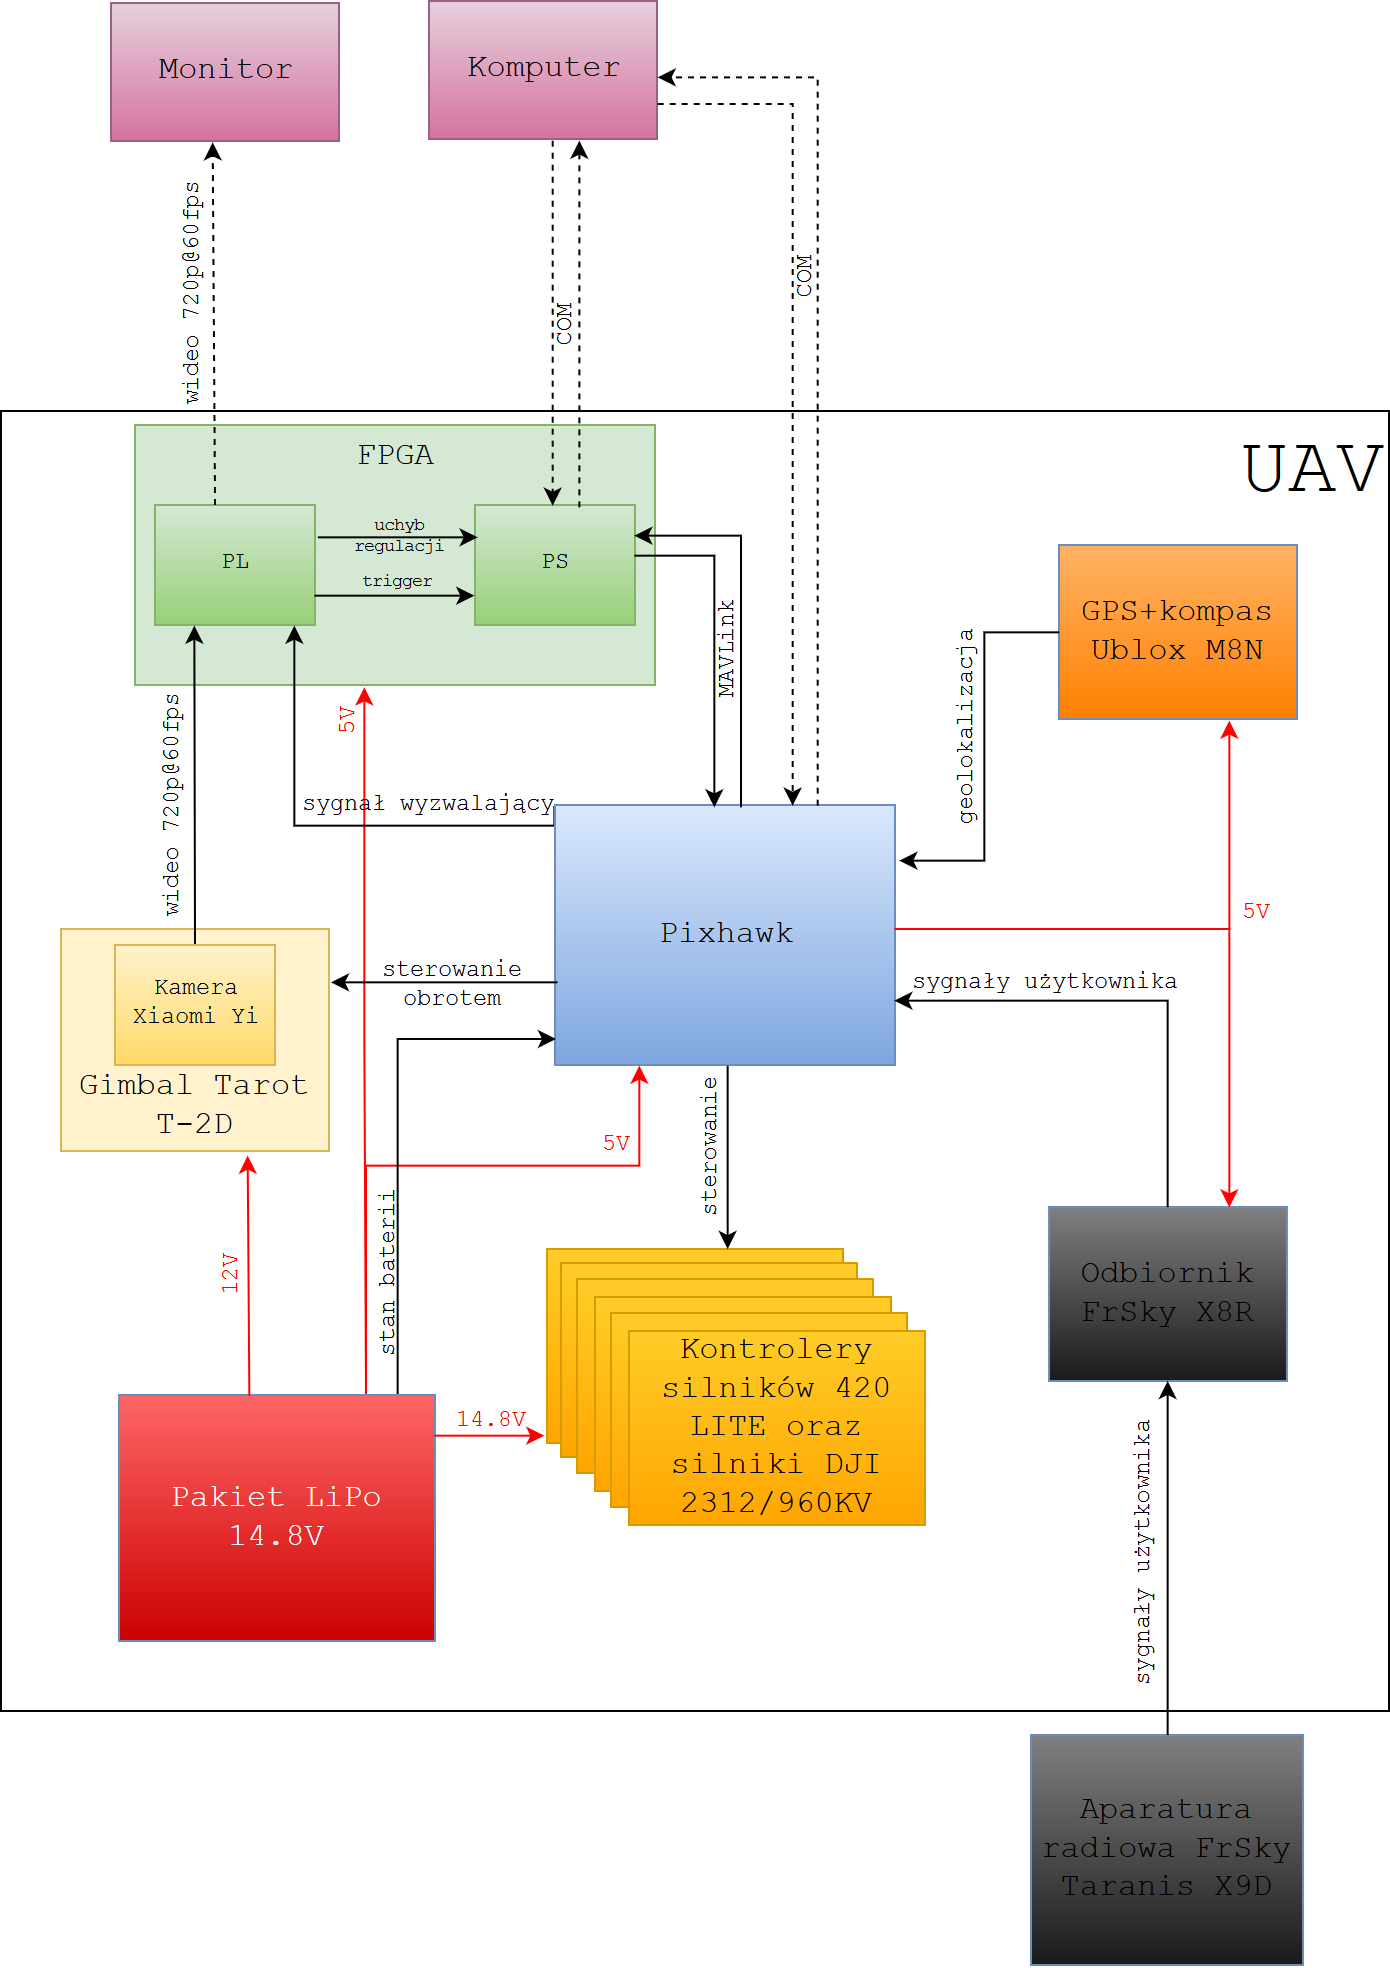
\includegraphics[width=14cm]{5_drone_architecture.png}
	\caption{Architektura sygnałowa tworzonego projektu}
	\label{fig:architecture}
\end{figure}

\section{Zdalne uruchomienie pracy systemu}

Początkowo stworzono (i ostatecznie pozostawiono) możliwość rozpoczęcia pracy z wykorzystaniem jednego z przełączników na płycie PYNQ, gdyż prace nad projektem wymagały dość częstego uruchamiania algorytmu jeszcze bez udziału drona. Jednak lot maszyny lub nawet jego start praktycznie wyklucza fizyczny dostęp do układu FPGA, dlatego koniecznością stało się zdalne wyzwolenie pracy algorytmów. Sygnał wyzwalający nosi nazwę \textit{trigger\char`_algorithm}.

Podczas lotu maszyny użytkownik ma pod ręką jedynie aparaturę radiową, z poziomu której może jednak w dość prosty sposób wystawiać sygnały. Aparatura jest bowiem wyposażona w szereg konfigurowalnych przełączników analogowych i cyfrowych. Ponadto, zdolna jest do transmisji 16 kanałów - przy czym do kontroli podstawowych funkcji drona wykorzystuje się zaledwie 4. Wybrano zatem jeden z pozostałych dostępnych kanałów, któremu przypisano funkcję trzypoziomowego przełącznika obecnego na panelu urządzenia radiowego.

Sparowany z aparaturą odbiornik wysyła wszystkie dane po jednym zestawie przewodów w formie PPM (ang. Pulse Position Modulation). Taki sygnał musiałby być zdekodowany w układzie FPGA do uzyskania użytecznej wartości. Proces dekodowania rozwiązuje jednak autopilot, który na podstawie 16-kanałowego PPM wystawia znacznie prostsze sygnały PWM (ang. Pulse Width Modulation) m.in. do kontroli silników. Co więcej, Pixhawk umożliwia przypisanie reszty kanałów transmisyjnych do pomocniczych wyjść PWM. Rozwiązanie to znalazło zastosowanie chociażby w ustawieniu wartości zadanych serwomechanizmom odpowiedzialnym za pracę gimbala kamery.

Ostatecznie kwestią niejasną pozostała szerokość pulsu, który miałby wyzwolić działanie algorytmu. O ile dla typowego sygnału PWM powinien on wynosić od 1ms do 2ms, to zdecydowano się ustalić wartość dla każdej z trzech pozycji przełącznika. Zastosowano w tym celu analizator logiczny ILA wbudowany w środowisko Vivado i stworzono prosty licznik, na którym stosuje się następujące operacje:
\begin{itemize}
	\item kasowanie na zboczu narastającym sygnału wejściowego,
	\item inkrementację podczas aktywnego stanu sygnału,
	\item przypisanie tej samej wartości w każdym innym przypadku.
\end{itemize}

Logika pracuje na zegarze \textit{calc\char`_clk} $=100$MHz i dla poszczególnych wartości przełącznika na aparaturze radiowej wartości licznika są przedstawione w poniższej tabeli. Pokazuje ona, że zakres długości pulsu nie odstaje od normy typowego sygnału PWM, mimo że jest nieco zawężony.

\newcolumntype{P}[1]{>{\centering\arraybackslash}p{#1}}
\begin{table}[h]
	\centering
	\begin{tabular}{|P{4cm} |P{3cm} |P{4cm}|}
		
		\hline
		\rowcolor{lightgray} Pozycja przełącznika & Wartość licznika & Długość pulsu [ms]  \\ 
		-1	& 109000 & 1.09	\\ 
		\hline
		0	& 149000 & 1.49 \\ 
		\hline
		1	& 189000 & 1.89 \\ 
		\hline
	\end{tabular}
	\caption{Szerokości pulsu PWM dla przełącznika odpowiedzialnego za start algorytmu}
	\label{tab:RFswitch}
\end{table}

Na tej podstawie określono, że warunkiem koniecznym do rozpoczęcia algorytmu będzie wystąpienie dwóch kolejnych pulsów o szerokości przynajmniej 1.8ms (górny limit przezornie ustawiono na 2ms). Analogicznie, zakończenie pracy algorytmu i powrót do ustawień domyślnych będzie miał miejsce dla dwóch pulsów o wartości spoza zakresu.

\section{Kontrola nad pracą algorytmów MeanShift oraz HoG+SVM}

Najwyższa warstwa w części programowalnej FPGA, łącząca pracę obu algorytmów, zarządza sygnałami mogącymi je niezależnie uruchomić. Zanim jednak przyjdzie na to pora, zadaniem maszyny stanu jest oczekiwanie na informację o gotowości drona, tj. ustabilizowaniu pozycji w powietrzu. 

Po otrzymaniu takiego sygnału kolejnym etapem jest pierwotna detekcja postaci. Wykorzystywany w tym celu algorytm HoG+SVM uruchamiany jest cyklicznie na przesuwanym oknie detekcji, by ostatecznie pokryć cały ekran. Każda ze skal dysponuje oknem detekcji o wymiarze $144\times 96$, z którego wybierany jest najlepszy fragment o wymiarach $128\times 64$. Porównując wielkość obu obszarów można dojść do wniosku, że jednorazowo pełnej analizie poddawanych jest jedynie $20\times 36$ pikseli - pozostałe muszą być wzięte pod uwagę przy analizie kolejnych okien. Jeśli odnieść poszczególne okna detekcji do oryginalnego rozmiaru obrazu, to oczywistym staje się, że najmniejsze pokrycie ma okno najmniejszego współczynnika skali:

\newcolumntype{P}[1]{>{\centering\arraybackslash}p{#1}}
\begin{table}[h]
	\centering
	\begin{tabular}{|p{1cm} |P{8cm}| P{5cm}|}
		
		\hline
		\rowcolor{lightgray} Skala & Rozmiar okna na oryginalnym obrazie & Przesunięcie \\ 
		\boldmath{$2$}	& \boldmath{$288\times 192$}	& \boldmath{$40\times 72$}  	\\ \hline
		$2.5$	& $360\times 240$ 	& nieistotne\\ \hline 			
		$3$	& $432\times 288$ 		& nieistotne\\ \hline
		$3.5$	& $504\times 336$	& nieistotne  	\\ \hline
		$4$	& $576\times 384$ 		& nieistotne\\ \hline

	\end{tabular}
	\caption{Wielkość jednorazowego pokrycia oknem detekcji dla wykorzystywanych skal}
	\label{tab:scale_window_cover}
\end{table}

Pierwszy obszar detekcji jest zlokalizowany w lewym górnym rogu - punkt centralny w $\{144,96\}$ - i porusza się horyzontalnie o zadaną w tabeli wartość. Po dotarciu do obszaru przy prawej krawędzi, cały proces jest powtarzany z przesunięciem wertykalnym - i tak osiągnięcia dolnej krawędzi obrazu. Przejście przez cały obraz $720\times 1280$ wymaga wykonania $11\cdot16=176$ iteracji algorytmu dla kolejnych nieparzystych klatek, co trwa nieco mniej niż 6 sekund. Proces ten może trwać krócej, jeśli kontroler natrafi na bardzo dobry wynik klasyfikacji, poniżej zadanego poziomu \textit{SVM\_strong\_threshold}=$-1$; w standardowej procedurze wystarczy zapamiętany najlepszy wynik poniżej \textit{SVM\_threshold}=$-0.1$.  Kolejny etap, weryfikacyjny, uruchamia się bezpośrednio po zakończeniu skanowania i uwzględnia przeprowadzenie 3 kolejnych iteracji SVM - w trybie śledzenia (analizując obszar z uwzględnieniem ostatniego wyniku SVM). Warunkiem przejścia przez ten etap jest, by wynik każdej iteracji był mniejszy od założonego maksimum \textit{SVM\_threshold}. W przeciwnym wypadku następuje powrót do etapu skanowania. 

Standardowe śledzenie opiera się na weryfikacji ostatniej iteracji, jednak proces uwzględnia jeszcze kilka elementów:
\begin{itemize}
	\item start algorytmu MeanShift - wcześniej niedostępny algorytm MS ma możliwość rozpoczęcia pracy po zarejestrowaniu dobrego wyniku klasyfikacji SVM (wartość mniejsza niż \textit{SVM\_strong\_threshold}). Wzorcem dla MS zostanie obszar z kolejnej klatki obrazu - kwadrat o środku w $\{x,y-30\}$ - gdzie $\{x,y\}$ to aktualny środek obszaru wyliczonego przez algorytm SVM. Podane przesunięcie w pionie pozwala rozpocząć śledzenie MS na obszarze w obrębie klatki piersiowej, wartość dobrano empirycznie.
	\item wyłączenie algorytmu MeanShift - MS może utracić zbieżność ze śledzonym obiektem, na przykład w związku ze zmianą oświetlenia. By się przed tym ustrzec, konieczne jest wyłączenie algorytmu, by w stosownym momencie ponownie go uruchomić. Odpowiedni warunek sprawdza, czy punkt MeanShift nie jest zbyt oddalony od punktu zwracanego przez poprawnie działający algorytm SVM.
	\item utrata śledzonego obiektu - jeśli wynik ostatniej klasyfikacji nie spełnia \textit{SVM\_threshold}, może to oznaczać potencjalną utratę śledzonej postaci z pola widzenia. Wówczas inicjatywa jest przejmowana przez algorytm MeanShift, którego wyniki stanowić będą wejście dla SVM (poprawione o wspomniany wyżej offset $30$). Warunkiem wyjścia z tego stanu (powrotu do standardowego śledzenia) jest osiągnięcie wyniku klasyfikacji rzędu \textit{SVM\_strong\_threshold}. Istotnym ograniczeniem jest ilość iteracji, w których ten tryb może pracować - domyślnie są to 2 sekundy (60 iteracji), jednak użytkownik może tę wartość modyfikować poprzez zapis do rejestru 0xC.
\end{itemize} 

\section{Komunikacja FPGA<->autopilot}
Wymiana informacji pomiędzy autopilotem a układem SoC bazuje na transmisji UART o standardowej prędkości równej 115200 bodów. Za transmisję po stronie układu SoC jest odpowiedzialna część PS, jednak istnieje możliwość lokalizacji sygnałów RxD oraz TxD po stronie części PL (wybór spośród większej ilości pinów). Z kolei na autopilocie skonfigurowano port TELEM 2.
Warstwą transportową jest protokół MAVLink, opracowany w 2009 roku na potrzeby małych bezzałogowych pojazdów. Dość duży podzbiór jego komend jest wspierany przez oprogramowanie ArduCopter (pełna lista jest dostępna pod adresem: \cite{ArduCopterCmds}). Ramka protokołu ma zmienną długość i jest opisana przez tabelę \ref{tab:MAVlinkframe}

\newcolumntype{P}[1]{>{\centering\arraybackslash}p{#1}}
\begin{table}[h]
	\centering
	\begin{tabular}{|P{1.5cm} |P{4cm}| p{9cm}|}
		
		\hline
		\rowcolor{lightgray} Bajt \# & Oznaczenie & Uwagi \\ 
		0	& Początek ramki &	Zawsze o wartości 254 \\ \hline
		1	& Długość danych & Wartość \textit{n} (w bajtach )	\\ \hline		
		2	& Sekwencja pakietu &	Wartość inkrementowana z każdą kolejną transmisją\\ \hline
		3	& ID systemu &	Dla komputera pokładowego (SoC) równa 255 \\ \hline
		4	& ID komponentu &	Dla komputera pokładowego (SoC) równa 190 \\ \hline
		5	& ID wiadomości &	\\ \hline
		6:n+6-1	& Dane & Struktura zależna od rodzaju wiadomości	\\ \hline
		n+6:n+7	& CRC &	Suma kontrolna całego pakietu bez bajtu \#0\\ \hline
	\end{tabular}
	\caption{Ramka protokołu MAVLink}
	\label{tab:MAVlinkframe}
\end{table}

Protokół został zaprojektowany w postaci plików nagłówkowych - taka forma umożliwia łatwe wykorzystanie w aplikacji tworzonej na jeden z procesorów ARM dostępnych na SoC ZYNQ.

\subsection{Aplikacja uruchomiona na procesorze ARM układu SoC ZYNQ}
O ile część PL układu ZYNQ jest tworzona w środowisku Xilinx Vivado, to narzędziem deweloperskim obsługującym PS jest inny program będący częścią suity Xilinxa - SDK (Software Development Kit). By jednak możliwe było rozpoczęcie pracy, konieczne jest zaimportowanie z Vivado tzw. konfiguracji sprzętowej, czyli informacji o dostępnych w PS peryferiach, oraz połączeniach pomiędzy PS a PL.

Jednym z nich jest GPIO, do którego podłączony został sygnał \textit{trigger\char`_algorithm}. Odpowiednio skonfigurowane GPIO może generować przerwania, co wykorzystano jako reakcję na włączenie bądź wyłączenie algorytmu.

Pozostałymi peryferiami są dwa interfejsy UART. Lokalizacją dla pierwszego interfejsu UART są dwa piny, które połączono z odpowiednim portem autopilota. Aplikacja, korzystając z biblioteki MAVLink jest w stanie zdekodować i sparsować ramki przychodzące, oraz odpowiednio spakować komendy wysyłane do autopilota.
\newline Drugi interfejs UART, wyprowadzony domyślnie na wyjście microUSB płyty PYNQ, stanowi połączenie z komputerem jako element różnorakich testów i debugowania w trakcie implementacji. Utworzono dla niego prostą formę terminala, który w odpowiedzi na komendy wpisywane z klawiatury komputera umożliwia zapis i odczyt z testowych rejestrów, wysyłanie określonych wiadomości do autopilota, ale przede wszystkim wyświetla odpowiednio sparsowane informacje wysyłane przez autopilot.

W aplikacji zaimplementowano nadrzędną maszynę stanu, której tempo pracy jest nadane przez odbierane co sekundę wiadomości z autopilota o ID=0, które noszą nazwę „Heartbeat”. Dzięki temu prostemu zabiegowi nie ma potrzeby korzystania z wewnętrznych liczników czy tworzenia funkcji opóźniających. Warunkiem pracy maszyny stanu jest obecność sygnału \textit{trigger\char`_algorithm}. Po jego zboczu narastającym następuje próba uzbrojenia drona; po zboczu opadającym procesor wyśle komendę rozpoczynającą proces lądowania. Bardziej szczegółowy opis komunikacji z dronem przedstawia schemat:

\begin{figure}[h]
	\centering
	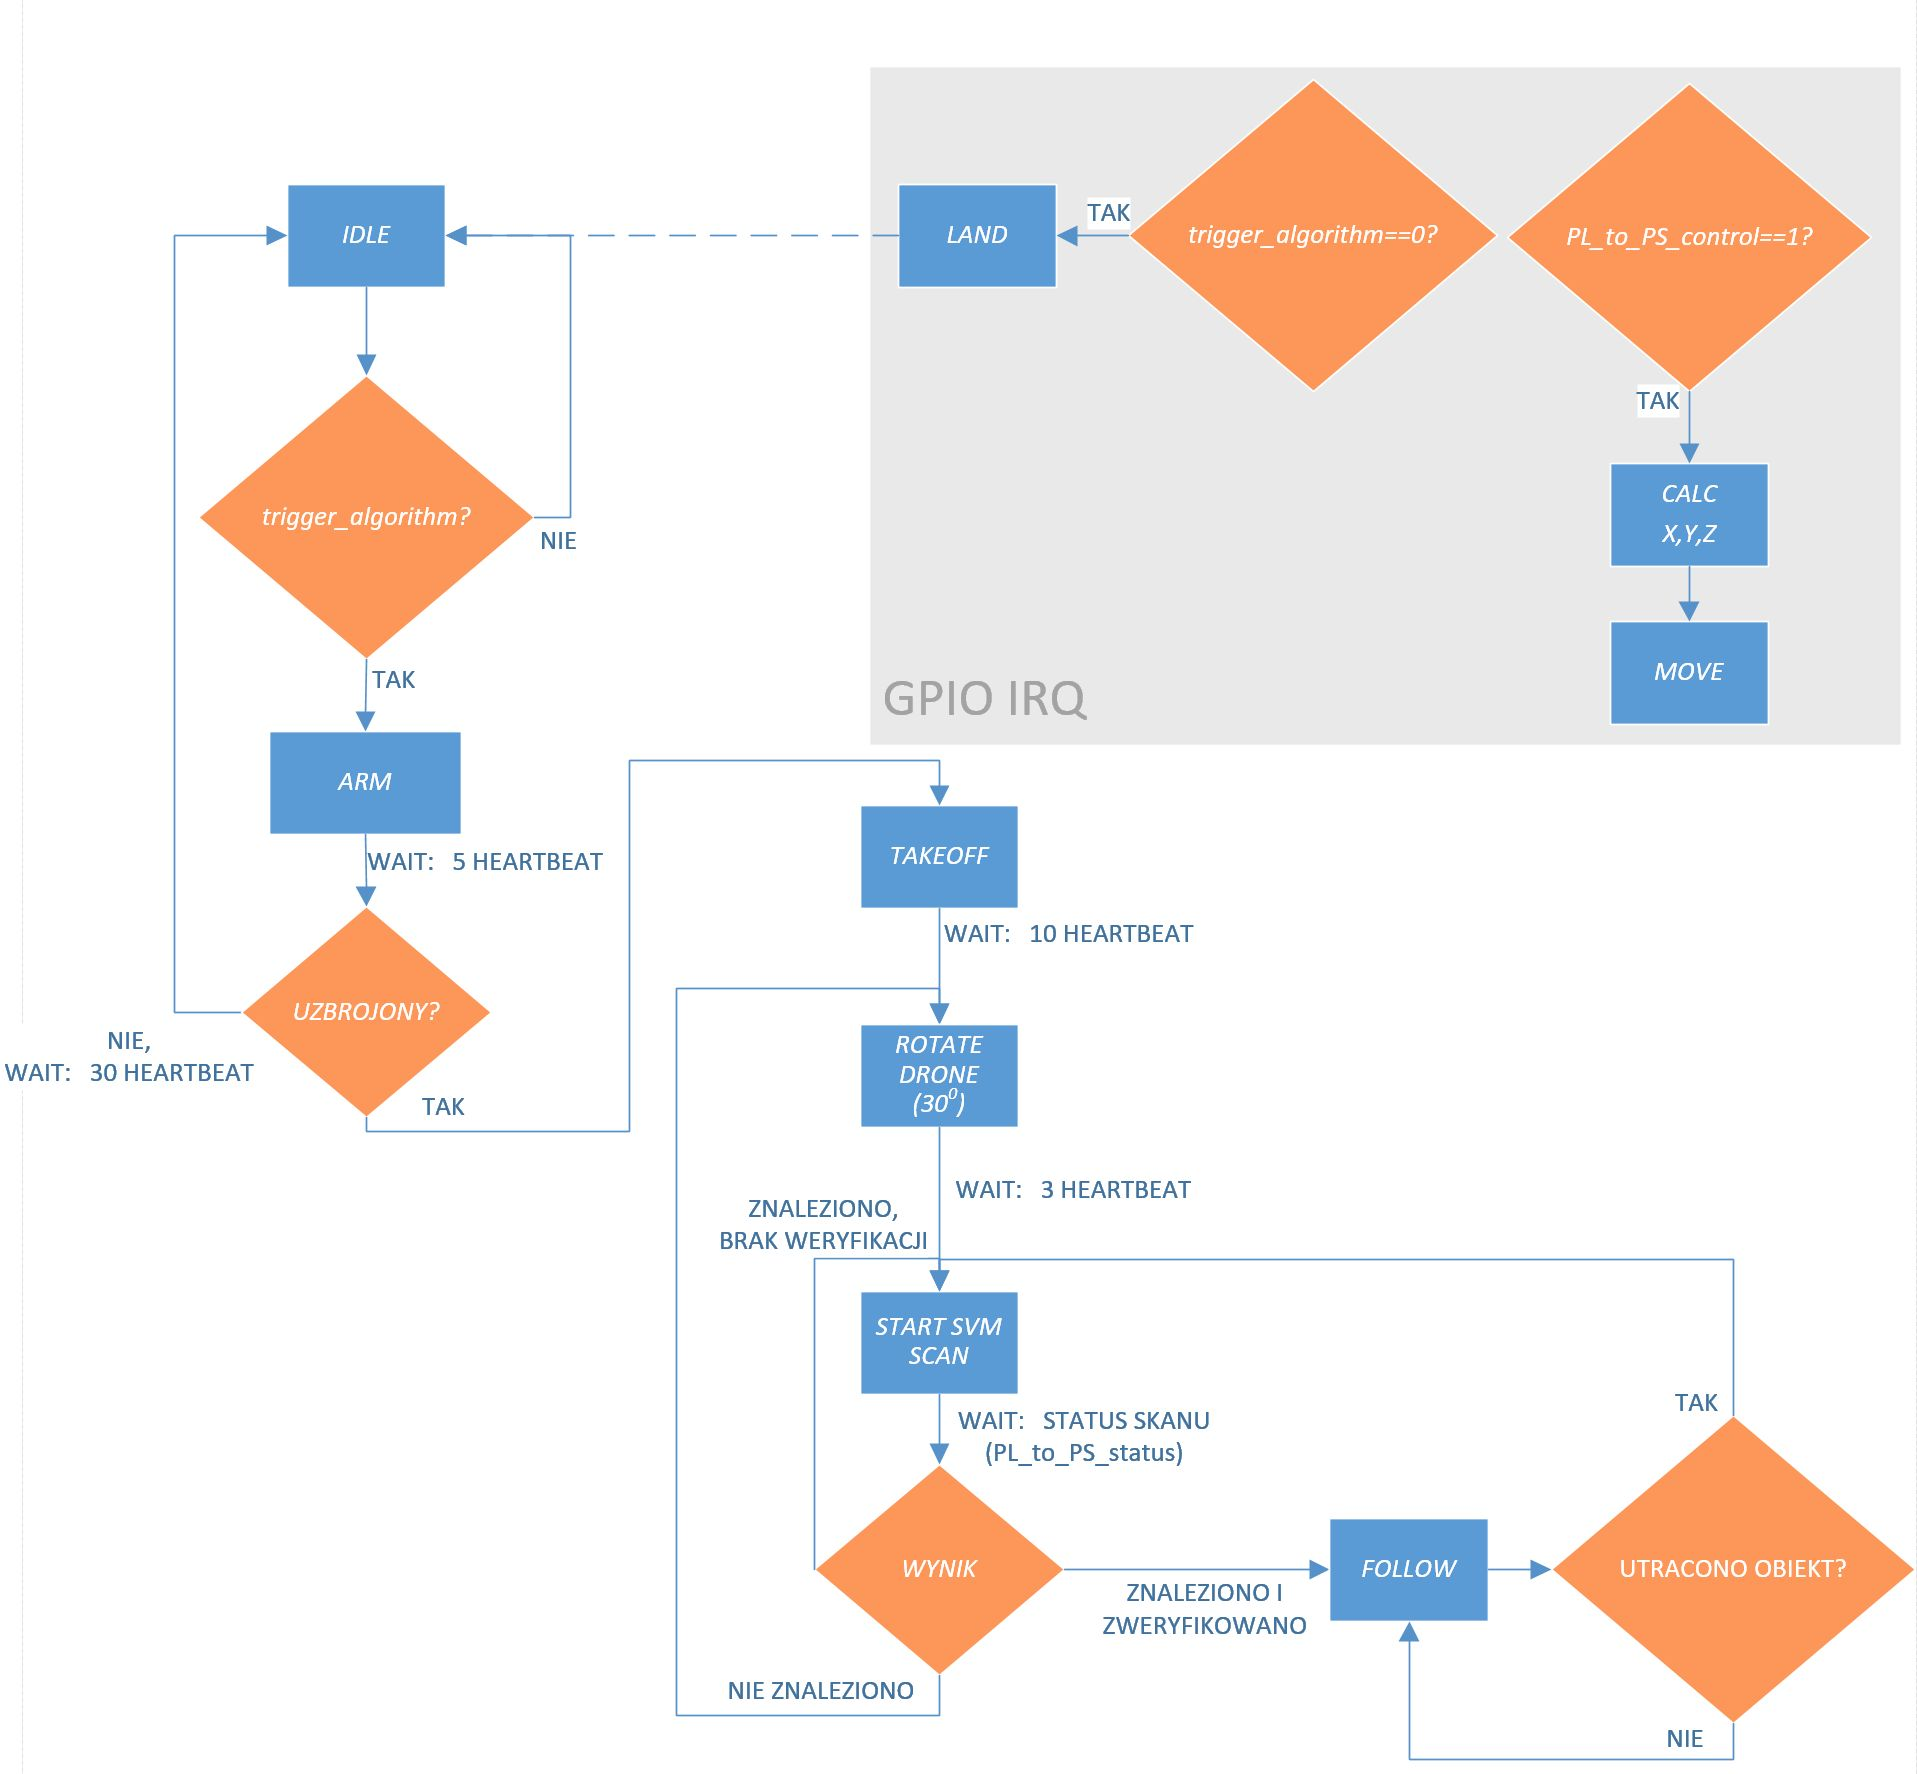
\includegraphics[width=16cm]{5_PS_FSM.jpg}
	\caption{Nadrzędny schemat działania systemu}
	\label{fig:PL_FSM_sch}
\end{figure}


\chapter{Testy}

Sprawdzenie poprawności działania obu algorytmów miało przebieg dwustopniowy:
\begin{itemize}
	\item symulacja modelu behawioralnego,
	\item uruchomienie algorytmu z warstwą sterującą na dronie.
\end{itemize}

\section{Testy symulacyjne}
O ile drugi ze sposobów był traktowany jako etap finalny, zwieńczający pracę nad projektem, to testy symulacyjne przebiegały równolegle z postępem prac nad poszczególnym z algorytmów śledzących. Co więcej, za wzór symulacji obrano uprzednio stworzony model programowy w MATLABie, chociażby ze względu na wykorzystanie tych samych obrazów w celu porównania wyników.
Moduł symulacyjny stworzony w środowisku Vivado i języku SystemVerilog nie uwzględniał jedynie części logiki zawartej w Block Designie - a więc instancji procesora oraz wejściowego i wyjściowego fragmentu toru wizyjnego. Byłaby to jednak część niepotrzebna, znacznie obciążająca i spowalniająca pracę symulatora. Jako zamiennik, wystarczył zasymulowany komplet sygnałów RGB z informacją o wartości piksela, która została wczytana z pliku tekstowego. Plik przechowujący jedną ramkę obrazu, wygenerowano w MATLABie umieszczając każdy kolejny pixel w nowej linii w formacie heksadecymalnym, po dwa znaki na każdą składową R, G i B.

Podstawowej funkcją symulacji jest możliwość podejrzenia propagowanych w układzie sygnałów w przystosowanym do tego oknie. Jednak ze względu na rozrastający się poziom skomplikowania modułów z czasem postanowiono bezpośrednio porównać wybrane funkcjonalności z pracą modelu programowego. W kodzie architektury stworzono logikę zapisującą do plików określone informacje z pojedynczej iteracji algorytmu. By jednak zapis nie był realizowany na każdym zboczu narastającym zegara, potrzebne było określenie sygnałów wyzwalających - zazwyczaj były to odpowiedniki sygnałów aktywnych. Do analizy stworzono w MATLABie dodatkowy skrypt, który parsował stworzone podczas symulacji pliki, uruchamiał pojedynczy przebieg modelu programowego i porównywał wyniki, określając ilość błędów na danym etapie algorytmu dla całej ramki. Niektóre dane, z racji ograniczenia bitowej reprezentacji w architekturze, wymagały zdefiniowania akceptowalnego poziomu tolerancji błędu.


\section{Testy na urządzeniu}

Symulacje są zbyt kosztownym czasowo narzędziem, dlatego w pewnym momencie należało przejść na testy na urządzeniu PYNQ. Proces budowy projektu sprowadza się do zbudowania konfiguracji sprzętowej w Vivado i skompilowaniu aplikacji uruchamianej na procesorze ARM. Docelowo układ SoC może być uruchomiony z poziomu karty SD, jednak ze względu na kwestię praktyczności, pozostano przy połączeniu JTAG. Stworzona konfiguracja testowa jest przedstawiona na schemacie.

\begin{figure}[h]
	\centering
	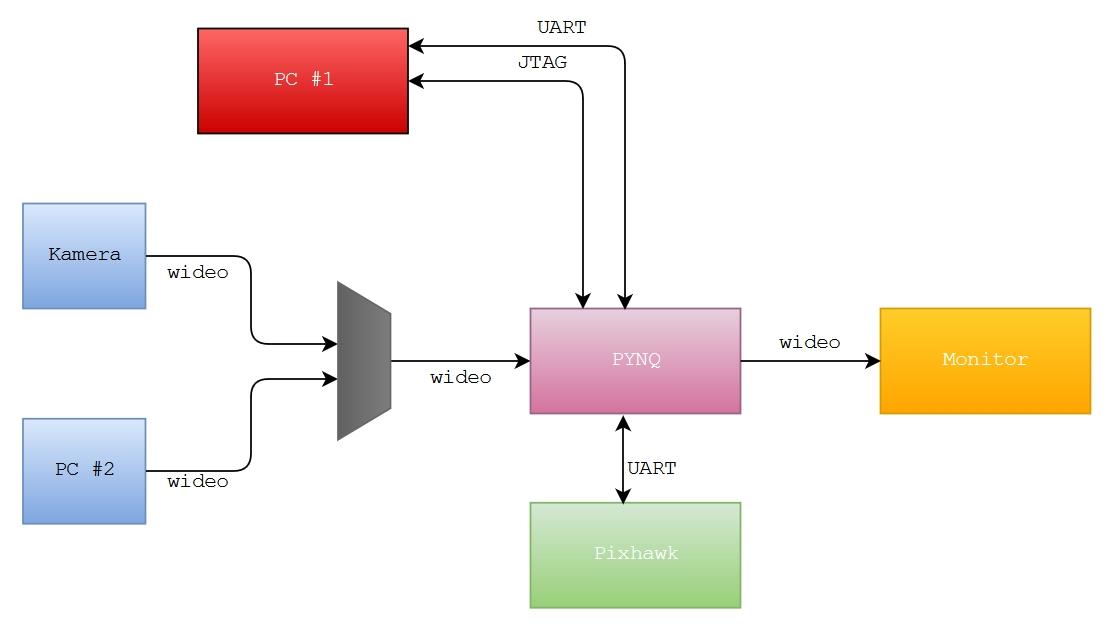
\includegraphics[width=16cm]{6_testing_setup.jpg}
	\caption{Schemat stanowiska testowego}
	\label{fig:testing_setup}
\end{figure}

Na przykładowym materiale wideo zaprezentowano skanowanie obrazu. Niebieskimi prostokątami oznaczone są aktualne okna detekcji dla poszczególnych skal. Zielone okno to obszar śledzenia algorytmem MeanShift, natomiast różowym kolorem oznaczono aktualnie najlepsze okno $128 \times 64$ (przeskalowane ponownie do oryginalnej rozdzielczości).

\begin{figure}[h]
	\centering
	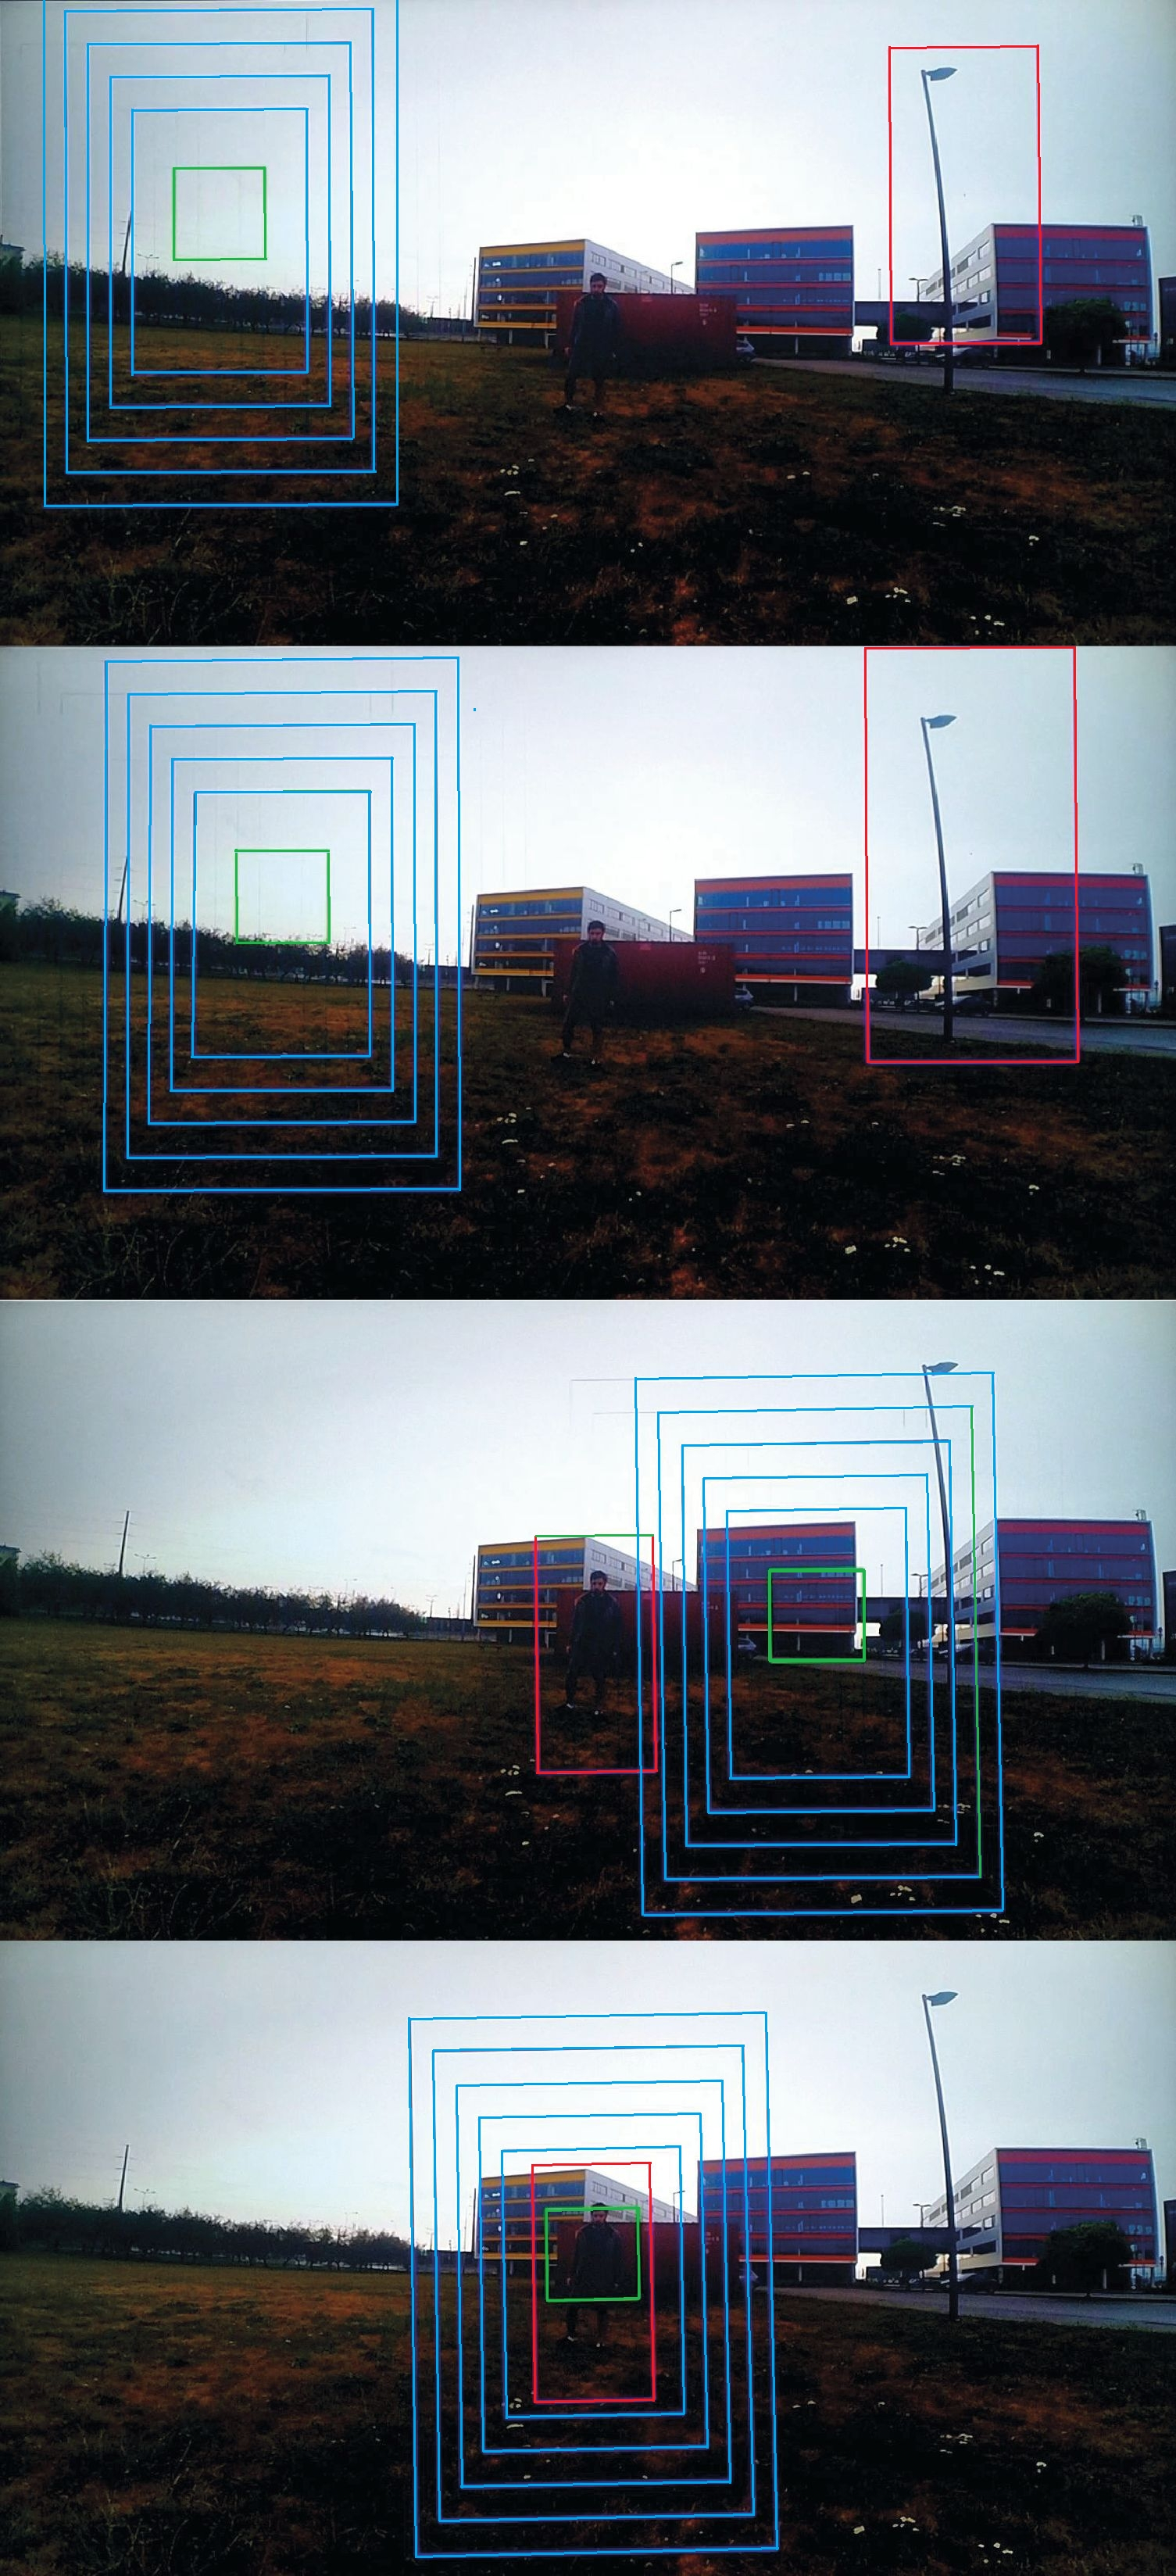
\includegraphics[width=10cm]{6_scan_1.jpg}
	\caption{Proces skanowania}
	\label{fig:scan_screenshot}
\end{figure}

\begin{figure}[h]
	\centering
	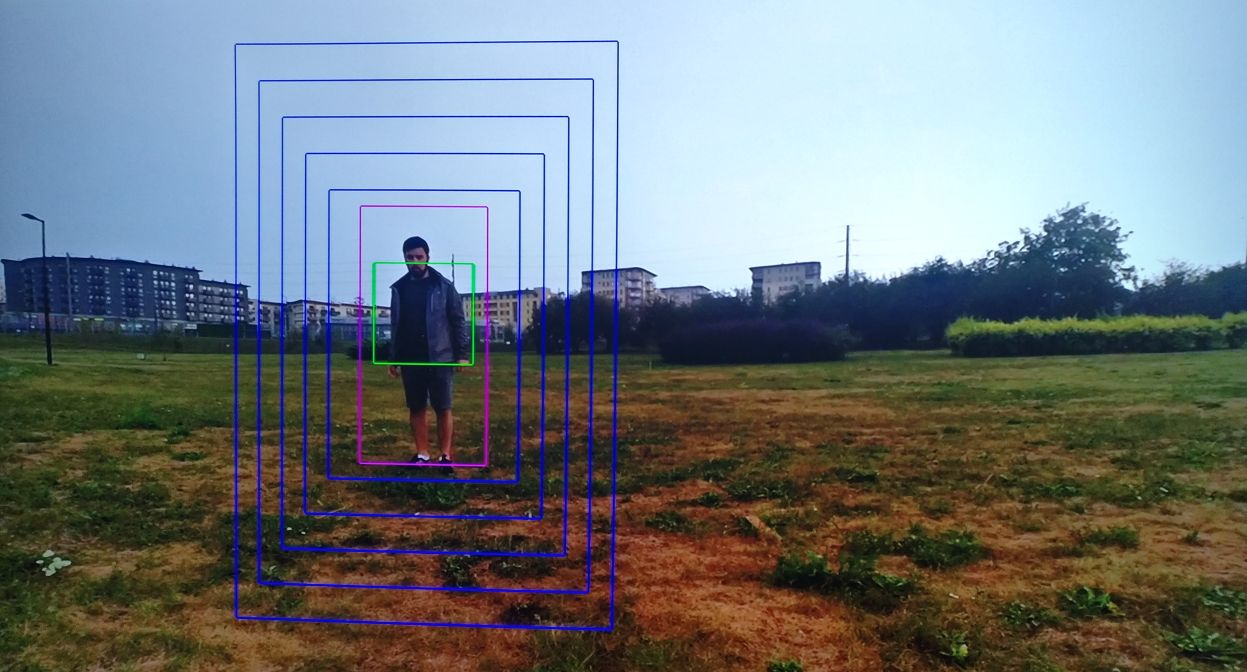
\includegraphics[width=10cm]{6_track_1.jpg}
	\caption{Śledzenie \#1}
	\label{fig:track_1}
\end{figure}

\begin{figure}[h]
	\centering
	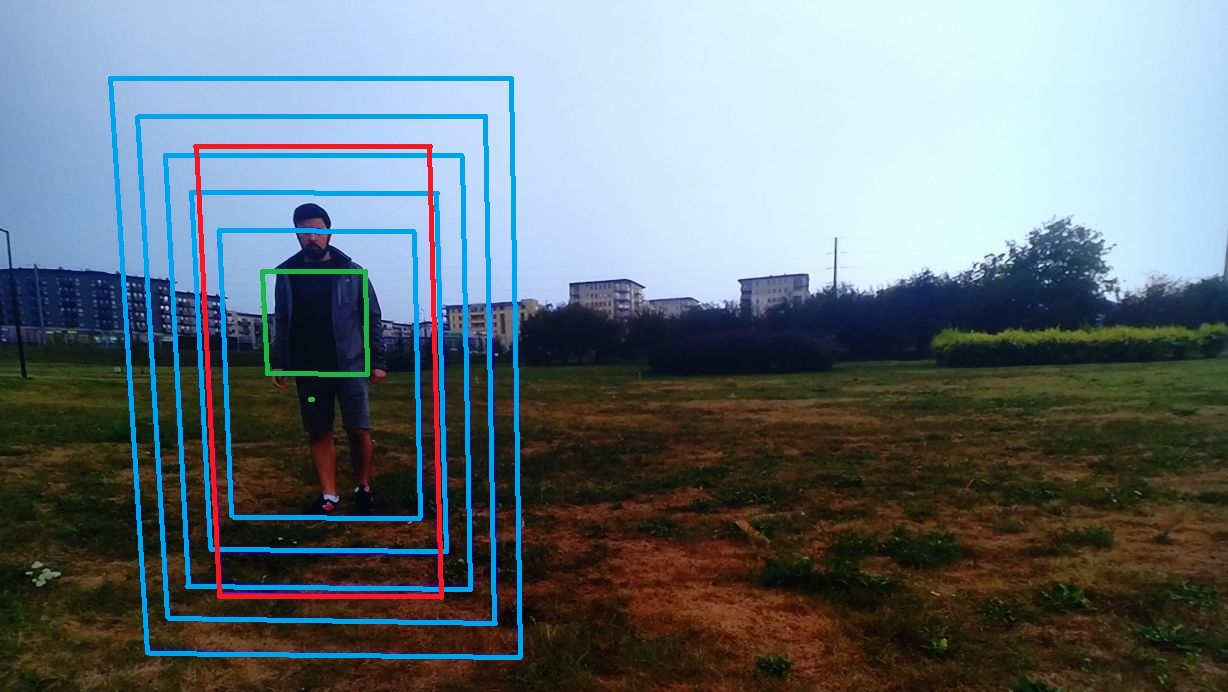
\includegraphics[width=10cm]{6_track_2.jpg}
	\caption{Śledzenie \#2}
	\label{fig:track_1}
\end{figure}

\begin{figure}[h]
	\centering
	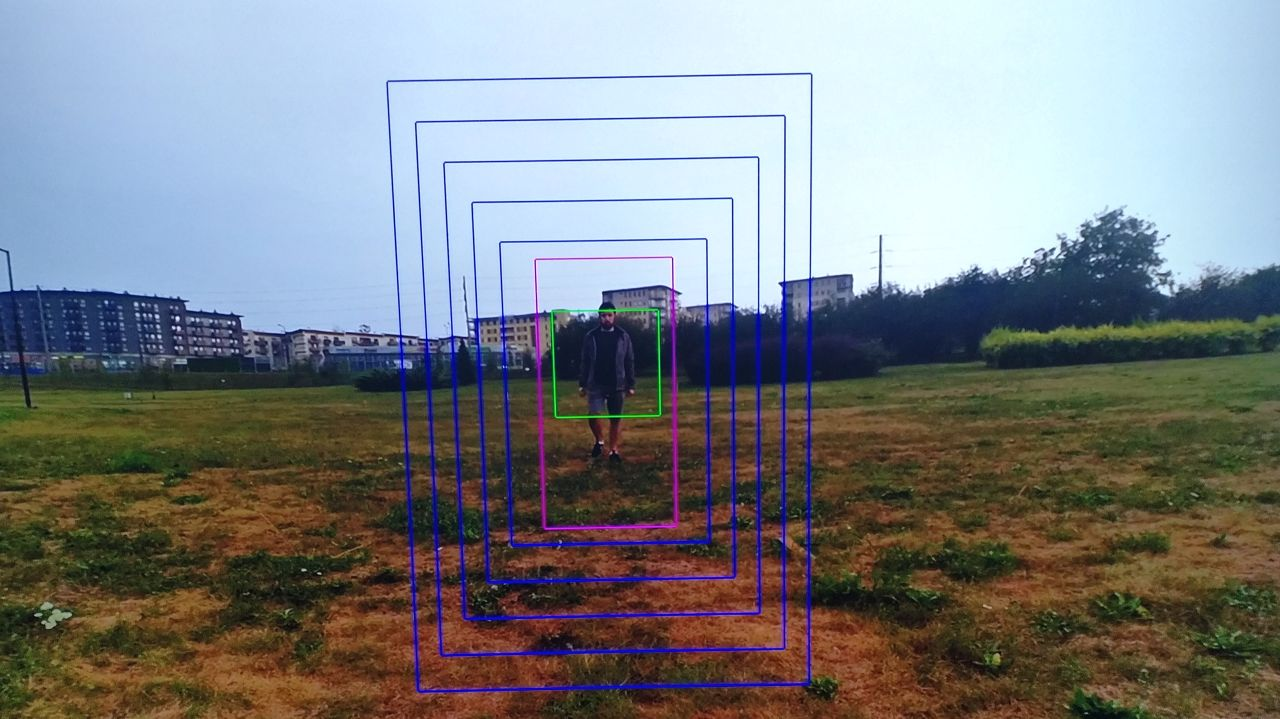
\includegraphics[width=10cm]{6_track_3.jpg}
	\caption{Śledzenie \#3}
	\label{fig:track_1}
\end{figure}

Szczególnie pomocne było wykorzystanie połączenia szeregowego z komputerem, by móc wyświetlić dodatkowe informacje przychodzące z autopilota. Większą część takiego raportu stanowi informacja z PL o odległości od wartości zadanej i skali - przemnożonej przez 10.


\begin{table}[h]
	\centering\scriptsize 
	
	\begin{tabular}{|p{8cm} |}
		
        \hline
prompt>>ARMING... \\
ARMED! \\
TAKING OFF... \\
Sent TAKEOFF CMD. \\
COMMAND ACK: 22 4 \\
STARTING SEARCH! \\
xDiff: 37        \tab yDiff: 33      \tab| scale: 27 || \\
DATA OK, STARTING FOLLOW! \\
xDiff: 20        \tab yDiff: 20      \tab| scale: 25 || \\
xDiff: 10        \tab yDiff: 20      \tab| scale: 25 || \\
xDiff: 52        \tab yDiff: 38      \tab| scale: 22 || \\
xDiff: 94        \tab yDiff: 8       \tab\tab| scale: 22 || \\
xDiff: 140       \tab yDiff: 12      \tab| scale: 20 || \\
xDiff: 165       \tab yDiff: 30      \tab| scale: 25 || \\
xDiff: 157       \tab yDiff: 22      \tab| scale: 22 || \\
xDiff: 125       \tab yDiff: 40      \tab| scale: 25 || \\
xDiff: 95        \tab yDiff: 35      \tab| scale: 22 || \\
xDiff: 62        \tab yDiff: 26      \tab| scale: 20 || \\
xDiff: 26        \tab yDiff: 28      \tab| scale: 20 || \\
xDiff: 10        \tab yDiff: 28      \tab| scale: 20 || \\
xDiff: -6         \tab\tab yDiff: 28      \tab| scale: 20 || \\
xDiff: -30        \tab yDiff: 36      \tab| scale: 20 || \\
xDiff: -70        \tab yDiff: 28      \tab| scale: 20 || \\
xDiff: -86        \tab yDiff: 20      \tab| scale: 20 || \\
xDiff: -118       \tab yDiff: 28      \tab| scale: 20 || \\
xDiff: -150       \tab yDiff: 12      \tab| scale: 20 || \\
xDiff: -150       \tab yDiff: 12      \tab| scale: 20 || \\
xDiff: -110       \tab yDiff: 20      \tab| scale: 20 || \\
xDiff: -86        \tab yDiff: 20      \tab| scale: 20 || \\
xDiff: -62        \tab yDiff: 28      \tab| scale: 20 || \\
INFO: PreArm: Throttle below Failsafe \\
xDiff: 22        \tab yDiff: 28      \tab| scale: 20 || \\
xDiff: 30        \tab yDiff: 4       \tab\tab| scale: 22 || \\
xDiff: 62        \tab yDiff: 42      \tab| scale: 27 || \\
xDiff: 95        \tab yDiff: 33      \tab| scale: 27 || \\
xDiff: 107       \tab yDiff: 33      \tab| scale: 30 || \\
xDiff: 107       \tab yDiff: 33      \tab| scale: 30 || \\
xDiff: 107       \tab yDiff: 33      \tab| scale: 30 || \\
xDiff: 172       \tab yDiff: 34      \tab| scale: 20 || \\
PARAM VAL: 0 1083785216 769  1898664 \\
PARAM VAL: 0 1091798652 769  1898664 \\
xDiff: 268       \tab yDiff: 14      \tab| scale: 20 || \\
xDiff: 368       \tab yDiff: 14      \tab| scale: 22 || \\
xDiff: 450       \tab yDiff: 20      \tab| scale: 25 || \\
xDiff: 560       \tab yDiff: 15      \tab| scale: 22 || \\
Sent LAND CMD. \\
COMMAND ACK: 21 0 \\    
\hline 	
	\end{tabular}
	\caption{Przykładowa zawartość terminala ze śledzenia na podstawie gotowego materiału wideo}
	\label{tab:log}
\end{table}
\chapter{Podsumowanie i możliwości rozwoju pracy}

W zrealizowanym projekcie przedstawiono sprzętową realizację detekcji i śledzenia osoby w heterogenicznym układzie ZYNQ SoC, na potrzeby kontroli bezzałogowego statku powietrznego. Osiągnięto przetwarzanie obrazu o rozdzielczości $1280\times 720$ dla 60 klatek na sekundę, z prędkością \textit{60Hz} i \textit{30Hz} odpowiednio dla algorytmów MeanShift oraz HoG+SVM.

Na uwagę zasługuje warstwa najwyższa, łącząca pracę obu algorytmów i komunikująca się z autopilotem Pixhawk. Wykorzystanie protokołu MAVLink pozwala stworzyć platformę, która jest w stanie wydawać polecenia ruchu bez udziału pilota.

Autor uważa jednak, że bazując na testowanej konfiguracji sprzętowo-programowej można dokonać szeregu usprawnień, podnoszących ogólną niezawodność rozwiązania. Jednym z nich jest próba zredukowania fałszywych detekcji (HoG+SVM) poprzez zmianę wielkości bloków lub komórek. Innym pomysłem mogłoby być proste zwiększenie analizowanych skal. Kolejnym usprawnieniem, tym razem dla algorytmu MeanShift, byłoby zlikwidowanie rzadkich sytuacji utraty zbieżności ze śledzonym obszarem - co skutkuje „wędrowaniem okna”. Barierą na drodze większości zmian jest liczba dostępnych zasobów w układzie - wymagana byłaby zmiana układu na dysponujący zwłaszcza większą ilością bloków BRAM. Istnieją jednak zmiany niewymagające ingerencji w kod. Do podstawowych należałoby lepsze skonfigurowanie kamery w celu poprawy rejestrowanych (wysyłanych kablem) kolorów. Kolejną mogłaby być lepsza stabilizacja obrazu. Ostatnią, mającą największy wpływ na śledzenie, byłoby poprawienie właściwości lotnych drona.

Ponadto, zbudowana platforma stanowi ogromny potencjał dla nowych pomysłów związanych z autonomizacją dronów. Podstawowym kierunkiem mogłaby być zdolność omijania przeszkód (nadal kosztowna opcja w dronach komercyjnych). Detekcja mogłaby być realizowana przez specjalistyczne czujniki, lub nawet LIDAR.\newline 




\appendix
\renewcommand{\thesection}{\Alph{section}}
\section{Spis zawartości płyty CD}

Dołączona do pracy płyta CD zawiera następujące pliki i katalogi:
\begin{itemize}
	\item praca.pdf - plik zawierający tekst pracy magisterskiej w formacie \textit{pdf},
	\item MATLAB - katalog zawierający pliki modelów programowych, a także pliki wideo służące do testów oraz zestaw treningowy SVM „INRIA Person dataset”,
	\item PYNQ - katalog zawierający projekt z plikami źródłowymi (PL oraz PS) do zbudowania i uruchomienia na układzie PYNQ,
	\item Praca\_TEX - katalog zawierający pliki \LaTeX z tekstem pracy magisterskiej oraz wykorzystanymi w niej rysunkami.
\end{itemize}


\printbibliography

\end{document}
